%%%%%%%%%%%%%%%%%%%%%%%%%%%%%%%%%%%%%%%%%%%%%%%%%%%%%%%%%%%%%%%%%%%%%%%%%%%%%%%%
%%
%%   BornAgain User Manual
%%
%%   homepage:   http://www.bornagainproject.org
%%
%%   copyright:  Forschungszentrum Jülich GmbH 2015
%%
%%   license:    Creative Commons CC-BY-SA
%%
%%   authors:    Scientific Computing Group at MLZ Garching
%%               C. Durniak, M. Ganeva, G. Pospelov, W. Van Herck, J. Wuttke
%%
%%%%%%%%%%%%%%%%%%%%%%%%%%%%%%%%%%%%%%%%%%%%%%%%%%%%%%%%%%%%%%%%%%%%%%%%%%%%%%%%

\part{Reference}\label{PREF}

\chapter{Form factor library}  \label{SFF}

% Don't number subfigures in this chapter.
\makeatletter
\renewcommand{\@thesubfigure}{\relax}
\makeatother

% \lstset{language=python,style=eclipseboxed,numbers=none,nolol}

\def\ffsection#1{\FloatBarrier\clearpage\ifodd\value{page}
\E{Page intentionally left blank}\clearpage\else\fi
\section{#1}}


\BornAgain\ comes with a comprehensive collection of hard-coded
shape transforms for standard particle geometries like
spheres, cylinders, prisms, pyramids or ripples.
This collection is documented in the following.
For each shape,
the real-space geometry is shown in orthogonal projections,
the parameters of the \BornAgain\ method are defined,
an analytical expression for the form factor is given,
and exemplary results for $\left|F(\q)\right|^2$ versus
$\alpha_\tf,\phi_\tf$ are shown for small-angle scattering conditions
($\alpha_\ti=\phi_\ti=0$).

The computation of $F(\q)$ is based on
shapes $S(\r)$ given in Cartesian coordinates,
as defined in the orthogonal projections.
Typically, the vertical ($z$) direction is chosen
along a symmetry axis of the particle.
The origin is always at the center of the bottom side of the particle.
Different parametrization or a different choice of the origin
cause our analytic form factors to trivially deviate
from expressions given in the \IsGISAXS\ manual \cite[Sec.~2.3]{Laz08}
or in the literature \cite[Appendix]{ReLL09}.

The particles can be rotated in a different direction by using one of
the following transformations: \Code{CreateRotateX($\theta$),
  CreateRotateY($\theta$), CreateRotateZ($\theta$)}, where capital X, Y, Z mark rotations
around the associated axis and $\theta$ is the
angle of rotation from this axis. For example, the following \Code{Python}\ script shows how to rotate a pyramid by $45^{\circ}$ around
the $z$-axis:\\

\begin{lstlisting}[language=python, style=eclipseboxed,numbers=none,nolol]
    pyramid_ff = FormFactorPyramid(10*nanometer, 5*nanometer, deg2rad(54.73 ) )
    pyramid = Particle(m_particle, pyramid_ff)
    angle_around_z = 45.*degree
    transform = Transform3D.createRotateZ(angle_around_z)
    particle_layout = ParticleLayout()
    particle_layout.addParticle(pyramid, transform)
\end{lstlisting}

\Tuto{Particle rotation is demonstrated in the example~\tuto{61}{rotated pyramids}.}

We recomputed all expressions to make sure
that they also hold for complex scattering vectors,
used to describe in order to take any material absorption into account.
The implementation in \BornAgain\ allows all three components
of~$\q$ to be complex.\footnote
{According to \cref{Smulayabs},
only the vertical components of $\k_\ti$ and $\k_\tf$ can have imaginary parts.
However,
for tilted particles
$F(\v{\tilde{q}})$ needs to be computed with
a rotated scattering vector~$\v{\tilde q}$
that may be complex in all three components.}
Some background information on the form factor computations is
given in \cref{SFFcomp}.

The following tables summarize the implemented particle geometries,
 roughly ordered by decreasing symmetry.
Afterwards, the detailed documentation is in alphabetical order.

%\clearpage\thispagestyle{empty}
\def\entry#1#2#3#4#5#6{%
\raisebox{-3.8ex}{\includegraphics[width=5em]{fig/blue/#2.png}} &
 \texttt{#1}& %\newline\textsl{#1} &
#5 & % symmetry
#4 & % parameters
Page~\pageref{S#3}\\} % , \cref{S#3}
\begin{center}
  \def\h{\text{h}}
  \def\v{\text{v}}
\small
\begin{longtable}
  {@{}p{.14\textwidth}
   @{}p{.32\textwidth}
   @{}p{.17\textwidth}
   @{}p{.19\textwidth}
   @{}p{.15\textwidth}@{}}
% Shape&{Name\newline \textsl{Legacy Name}}&Symmetry&Parameters&Reference\\\hline
Shape&Name&Symmetry&Parameters&Reference\\\hline
\entry{FullSphere}{FullSphere3d}{FullSphere}{$R$}{R$_3$}{Sphere}
\entry{FullSpheroid}{FullSpheroid3d}{FullSpheroid}{$R$, $H$}{D$_{\infty\h}$}{Spheroid}
\entry{Cylinder}{Cylinder3d}{Cylinder}{$R$, $H$}{D$_{\infty\h}$}{Cylinder}
\entry{TruncatedSphere}{Sphere3d}{TruncatedSphere}{$R$, $H$}{C$_{\infty\v}$}{SphericalCap}
\entry{TruncatedSpheroid}{Spheroid3d}{TruncatedSpheroid}{$R$, $H$, $f_p$}{C$_{\infty\v}$}{SpheroidalCap}
\entry{Cone}{Cone3d}{Cone}{$R$, $H$, $\alpha$}{C$_{\infty\v}$}{ConicalFrustum}
\entry{Icosahedron}{Icosahedron3d}{Icosahedron}{$L$}{I$_\h$}{Icosahedron}
\entry{Dodecahedron}{Dodecahedron3d}{Dodecahedron}{$L$}{I$_\h$}{Dodecahedron}
\entry{TruncatedCube}{TruncatedCube3d}{TruncatedCube}{$L$, $t$}{O$_\h$}{TruncatedCube}
\entry{Prism6}{Prism63d}{Prism6}{$R$, $H$}{D$_{6\h}$}{Prism6}
\entry{Cone6}{Cone63d}{Cone6}{$R$, $H$, $\alpha$}{C$_{6\v}$}{Frustum6}
\entry{Pyramid}{Pyramid3d}{Pyramid}{$L$, $H$, $\alpha$}{C$_{4\v}$}{Frustum4}
\entry{Cuboctahedron}{Cuboctahedron3d}{Cuboctahedron}{$L$, $H$, $r_H$, $\alpha$}{C$_{4\v}$}{BiFrustum4}
\entry{Prism3}{Prism33d}{Prism3}{$L$, $H$}{D$_{3\h}$}{Prism3}
\entry{Tetrahedron}{Tetrahedron3d}{Tetrahedron}{$L$, $H$, $\alpha$}{C$_{3\v}$}{Frustum3}
\entry{EllipsoidalCylinder}{EllipsoidalCylinder3d}{EllipsoidalCylinder}{$R_a$, $R_b$, $H$}{D$_{2\h}$}{EllipsoidalCylinder}
\entry{Box}{Box3d}{Box}{$L$, $W$, $H$}{D$_{2\h}$}{Prism2}
\entry{HemiEllipsoid}{HemiEllipsoid3d}{HemiEllipsoid}{$R_a$, $R_b$, $H$}{C$_{2\v}$}{HemiEllipsoid}
\entry{AnisoPyramid}{AnistropicPyramid3d}{AnisoPyramid}{$L$, $W$, $H$, $\alpha$}{C$_{2\v}$}{Frustum2}
\entry{Ripple1}{Ripple13d}{Ripple1}{$L$, $W$, $H$}{C$_{2\v}$}{Sinewave}
\entry{Ripple2}{Ripple23d}{Ripple2}{$L$, $W$, $H$, $d$}{C$_\text{s}$}{Sawtooth}
\hline
\end{longtable}
\end{center}
%\thispagestyle{empty}\clearpage

\index{Rotation of particles}
\index{Orientation of particles}
\index{CreateRotateX@\Code{CreateRotateX|Y|Z}}
\index{Transform3D@\Code{Transform3D}}

In the following subsections,
information about the implemented geometries is given in standardized form.
Analytical expressions are given for the form factor $F(\q)$,
for the volume $V=F(0)$,
and for the maximum horizontal section $S$
(the area of the particle as seen from above).
\nomenclature[2s130 0]{$S$}{Maximum horizontal section of embedded particle}%
Mathematical notation in the form factor expressions includes
the cardinal sine functions $\sinc(z)\coloneqq\sin(z)/z$
and the Bessel function of first kind and first order $J_1(z)$
\cite[Ch.~9]{AbSt64}.
\nomenclature[2j132 01]{$J_1$}{Bessel function of first kind and first order}%
If results contain an integral,
then no analytical form was found,
and the integral is evaluated by numeric quadrature.
\index{Quadrature}%
For polyhedral figures,
\index{Polyhedron!form factor}
\index{Form factor!polyhedron}
except a few simple ones like the rectangular box,
we use a generic form factor computation,
parametrized by the vertices of the figure,
that is described in full detail in a mathematical paper~\cite{ba:ffp}.

Almost all analytical expressions for $F(\q)$ contain
removable singularities for certain values of $\q$.
Our implementation uses proper analytic continuations at these singularities,
\index{Form factor!singularities}
\index{Singularitiy!in form factor computation}
though this is not explicitly denoted in the following formula collection.
Furthermore, series expansions are used to ensure numeric accuracies
in the neighborhood of the singularities.
For polyhedra, see Ref.~\cite{ba:ffp} for a meticulous discussion.

\begin{figure}[t]
\begin{center}
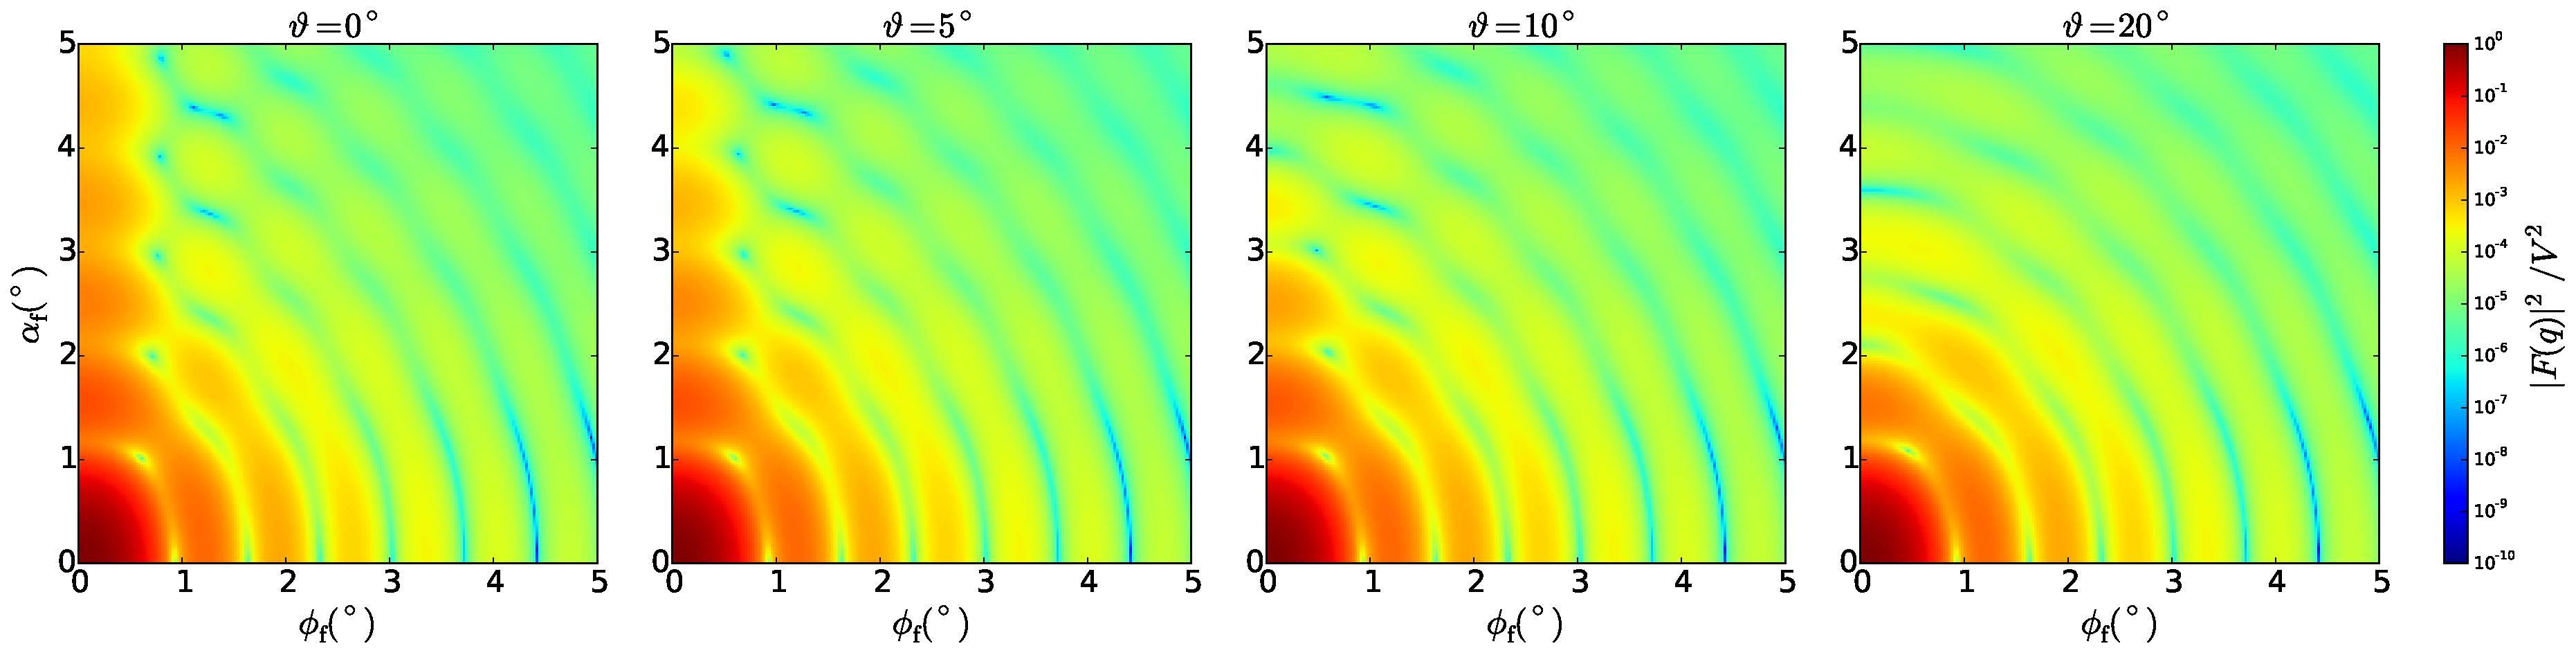
\includegraphics[width=\textwidth]{fig/ff2/ff_demo_1quadrants.pdf}
\end{center}
\caption{Normalized intensity $I(\alpha_\tf,\phi_\tf)$
for small-angle scattering by a truncated sphere with $R=4.2$~nm and $H=6.1$~nm,
for four different tilt angles~$\vartheta$ (rotation around the $y$ axis).
Since $I$ possess the standard symmetry (\protect\ref{EFq4sym}),
data are only shown for first quadrant $0^\circ\le\phi_\tf,\alpha_\tf\le 5^\circ$.}
\label{F1quadrants}
\end{figure}

Geometrical objects can be parametrized in different ways.
Concerns about user experience and about code readability
sometimes lead to different choices.
For the \BornAgain\ user interfaces (GUI and API)
we have chosen the most standard parameters,
as used in elementary geometry, like length, height, radius,
even if this is at variance from the \IsGISAXS\ precedent.
Where our parametrization made analytic expressions too tedious,
we use alternate internal parameters to alleviate the formul\ae.

Examplary form factors are numerically computed in Born approximation.
The particles are assigned a refractive index of $n=10^{-5}$.
Parameters are chosen such that
the particle volume~$V$ is about 250~nm$^3$ (within $\pm5$~\%);
except ripples, which are chosen with a vertical section $V/L$ of 40~nm$^2$
and a length of 25~nm.
The incident wavelength is 1~\AA.
The incident beam is always in $x$ direction, hence $\alpha_\ti=\phi_\ti=0$.
Simulated detector images are normalized to the maximum scattering intensity at $F(0)=V$,
\begin{equation}
  I(\alpha_\tf,\phi_\tf)\coloneqq |F(q(\alpha_\tf,\phi_\tf))|^2/V^2.
\end{equation}
All plots have the same logarithmic color scale,
extending over ten decades from $10^{-1)}$ to~1.
Plot ranges in $\alpha_\tf$ and $\phi_\tf$ are also standardized as far as
reasonably possible.
For most particle geometries,
$I$ has horizontal and vertical mirror planes:
\begin{equation}\label{EFq4sym}
  I(\alpha_\tf,\phi_\tf)
  = I(\alpha_\tf,-\phi_\tf)
  = I(-\alpha_\tf,-\phi_\tf)
  = I(\alpha_\tf,-\phi_\tf).
\end{equation}
% TODO RESTORE TEMPORARILY REMOVED XREF
% The physical origin this symmetry is discussed in \cref{Ssym}.
For these particles,
plots of $I$ are restricted to the quadrant $\alpha_\tf\ge0$, $\phi_\tf\ge0$.
However, it requires some experience to fully appreciate the
information content of these plots.
For a demonstration of this,
try to capture the main features of \cref{F1quadrants}.
Then compare with \cref{F4quadrants}.

\begin{figure}[t]
\begin{center}
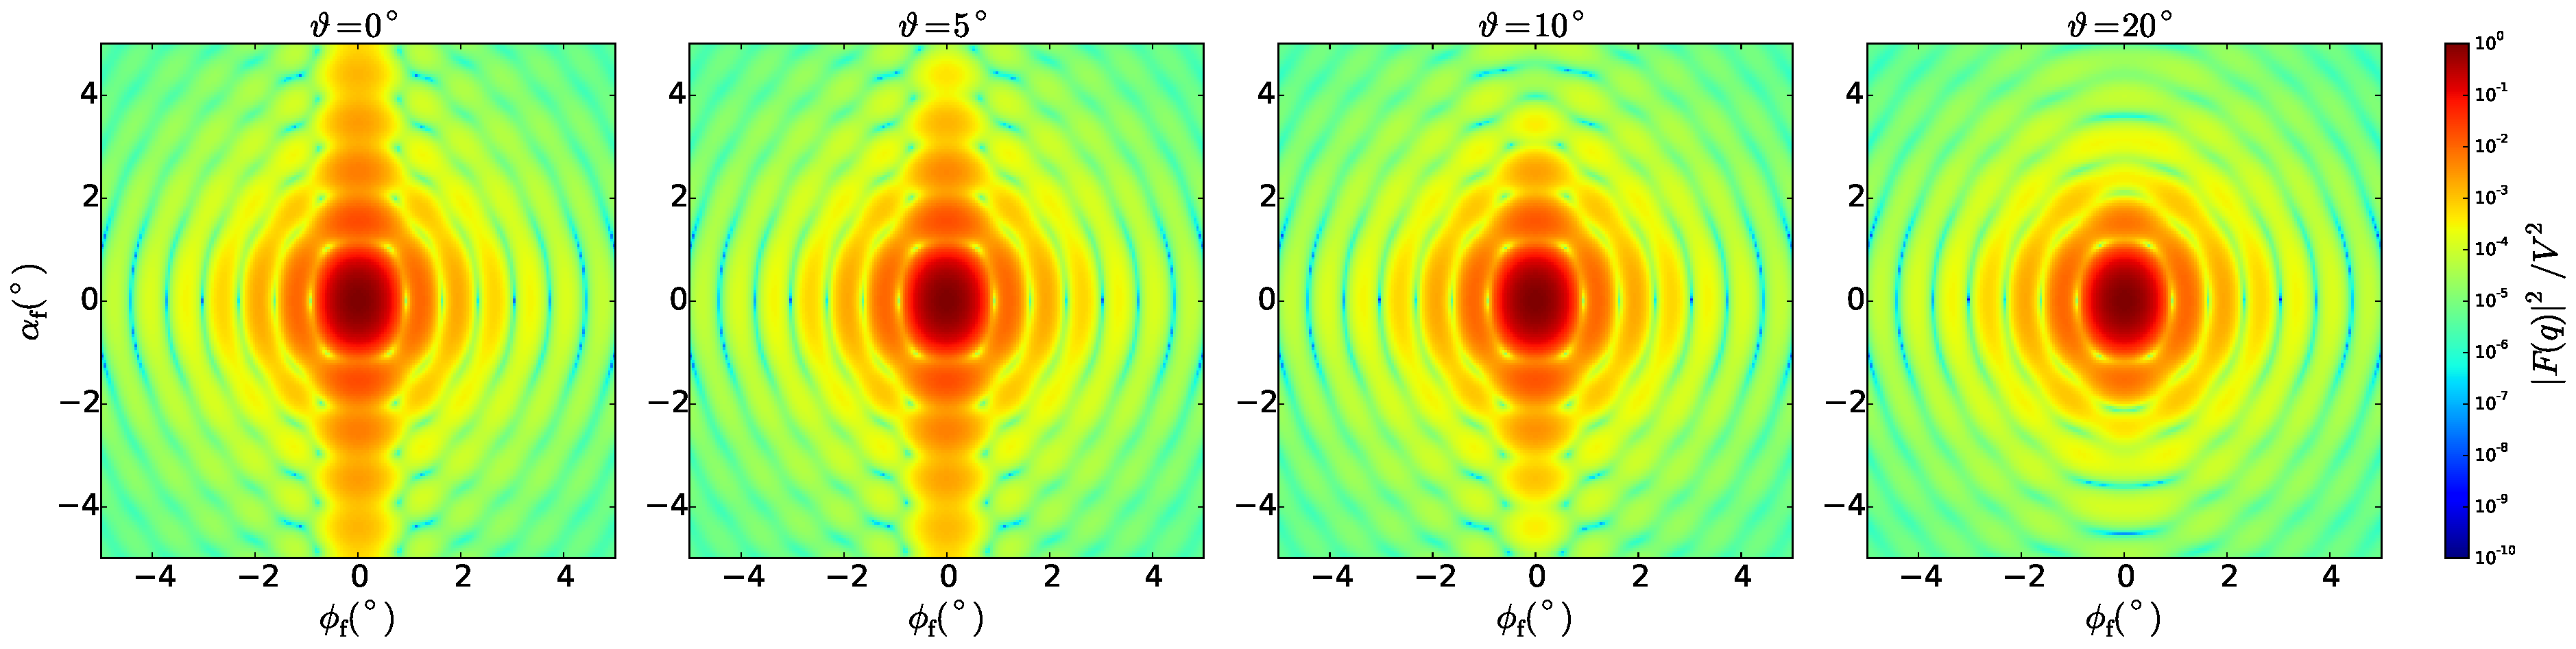
\includegraphics[width=\textwidth]{fig/ff2/ff_demo_4quadrants.pdf}
\end{center}
\caption{Same data as in Fig.~\protect\ref{F1quadrants},
but now shown for all four quadrants ($-5^\circ\le\phi_\tf,\alpha_\tf\le 5^\circ$).
The vertical interference pattern,
which gradually disappears with increasing tilt angle,
 is much more salient in this plot
than in the preceding one-quadrant representation.}
\label{F4quadrants}
\end{figure}

\index{Shape transform!catalogue|(}
\index{Form factor!catalogue|(}

%===============================================================================
\ffsection{AnisoPyramid (rectangle-based)} \label{SAnisoPyramid}
%===============================================================================
  \index{Anisotropic pyramid (form factor)}
  \index{Pyramid (form factor)!rectangular (AnisoPyramid)}
  \index{Truncated pyramid (form factor)!rectangular (AnisoPyramid)}
  \index{FormFactorAnisoPyramid@\Code{FormFactorAnisoPyramid}}

\paragraph{Real-space geometry}\strut\\

\begin{figure}[H]
\hfill
\subfigure[Perspective]{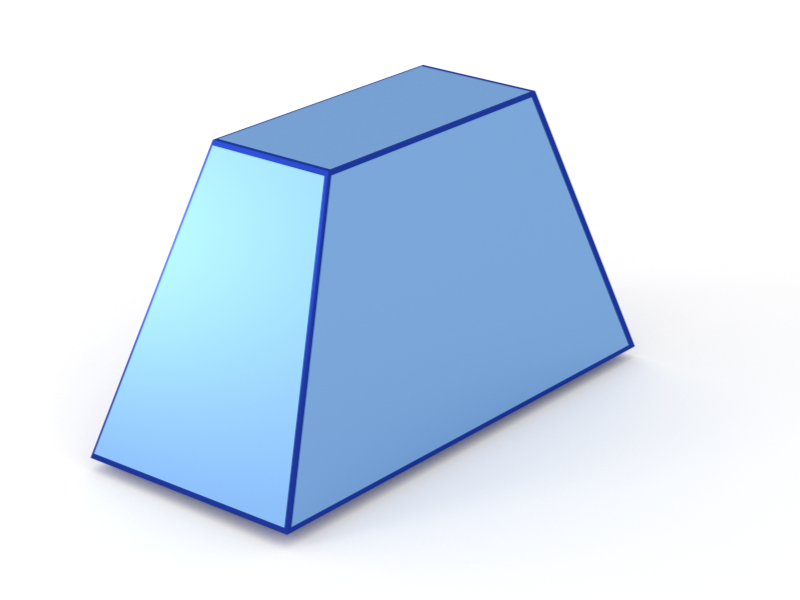
\includegraphics[width=.24\textwidth]{fig/blue/AnistropicPyramid3d.png}}
\hfill
\subfigure[Top view]{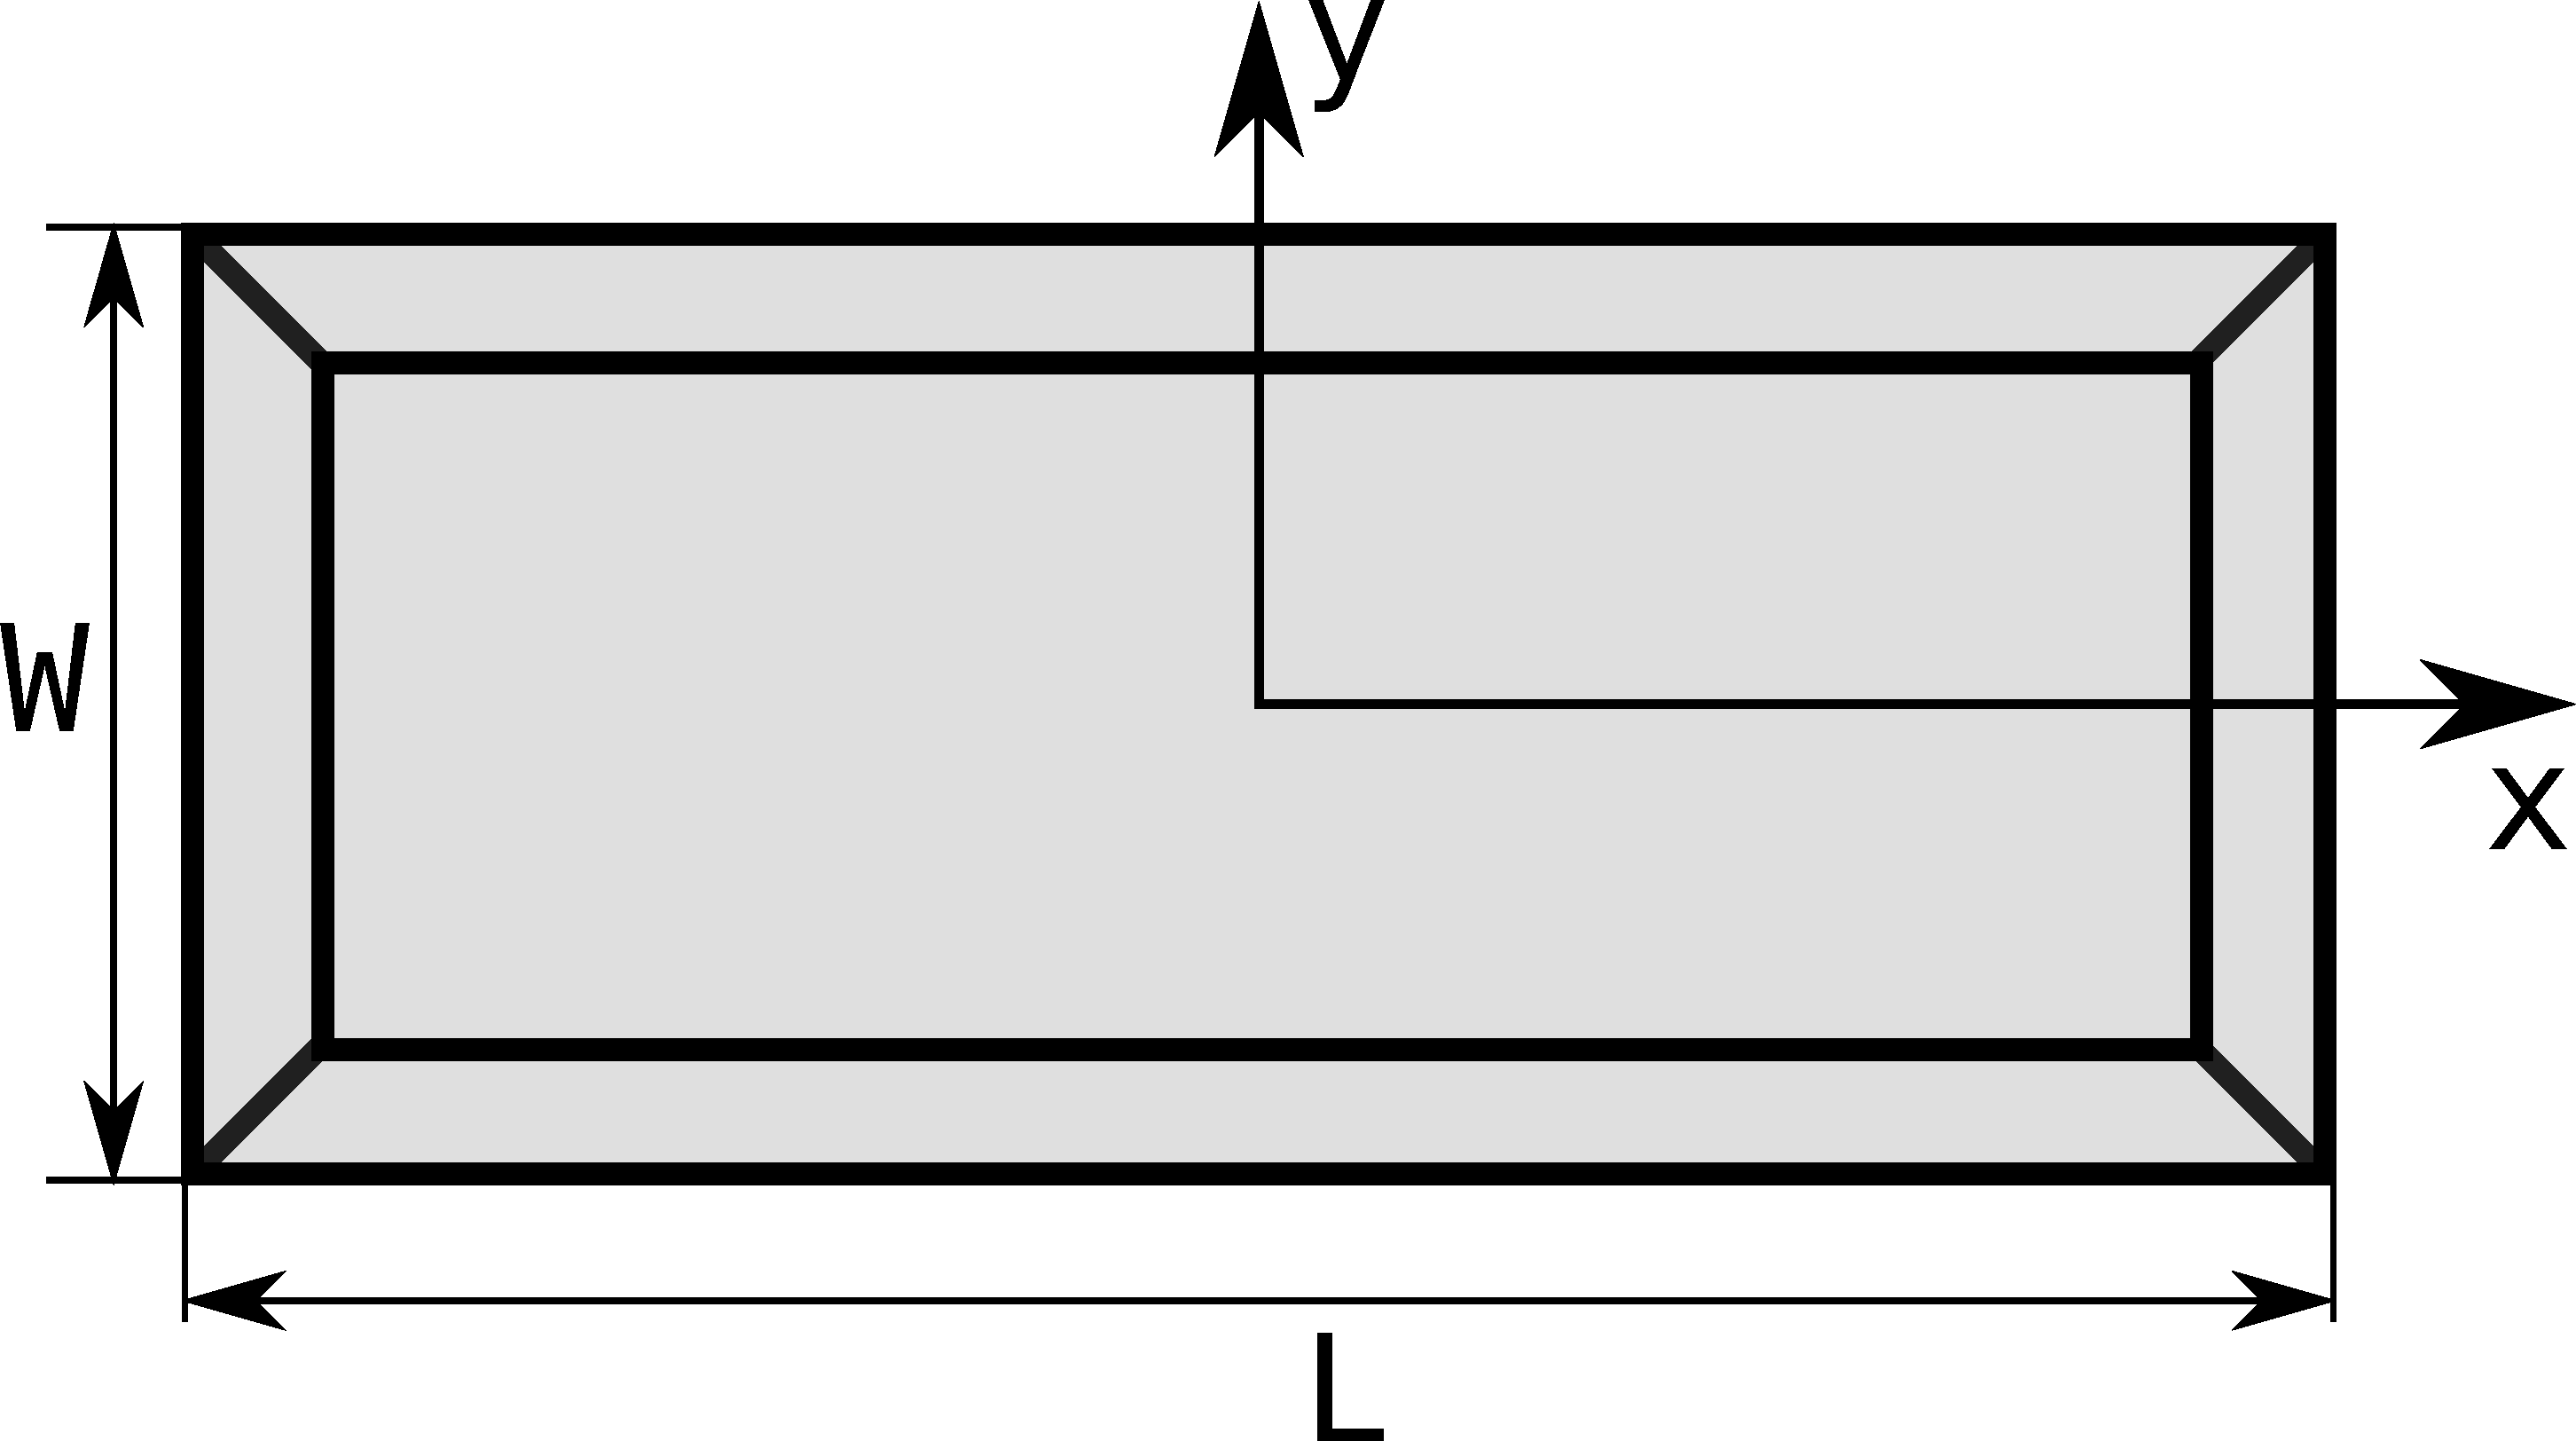
\includegraphics[width=.30\textwidth]{fig/cuts/AnisoPyramid2dxy.pdf}}
\hfill
\subfigure[Side view]{\raisebox{2mm}{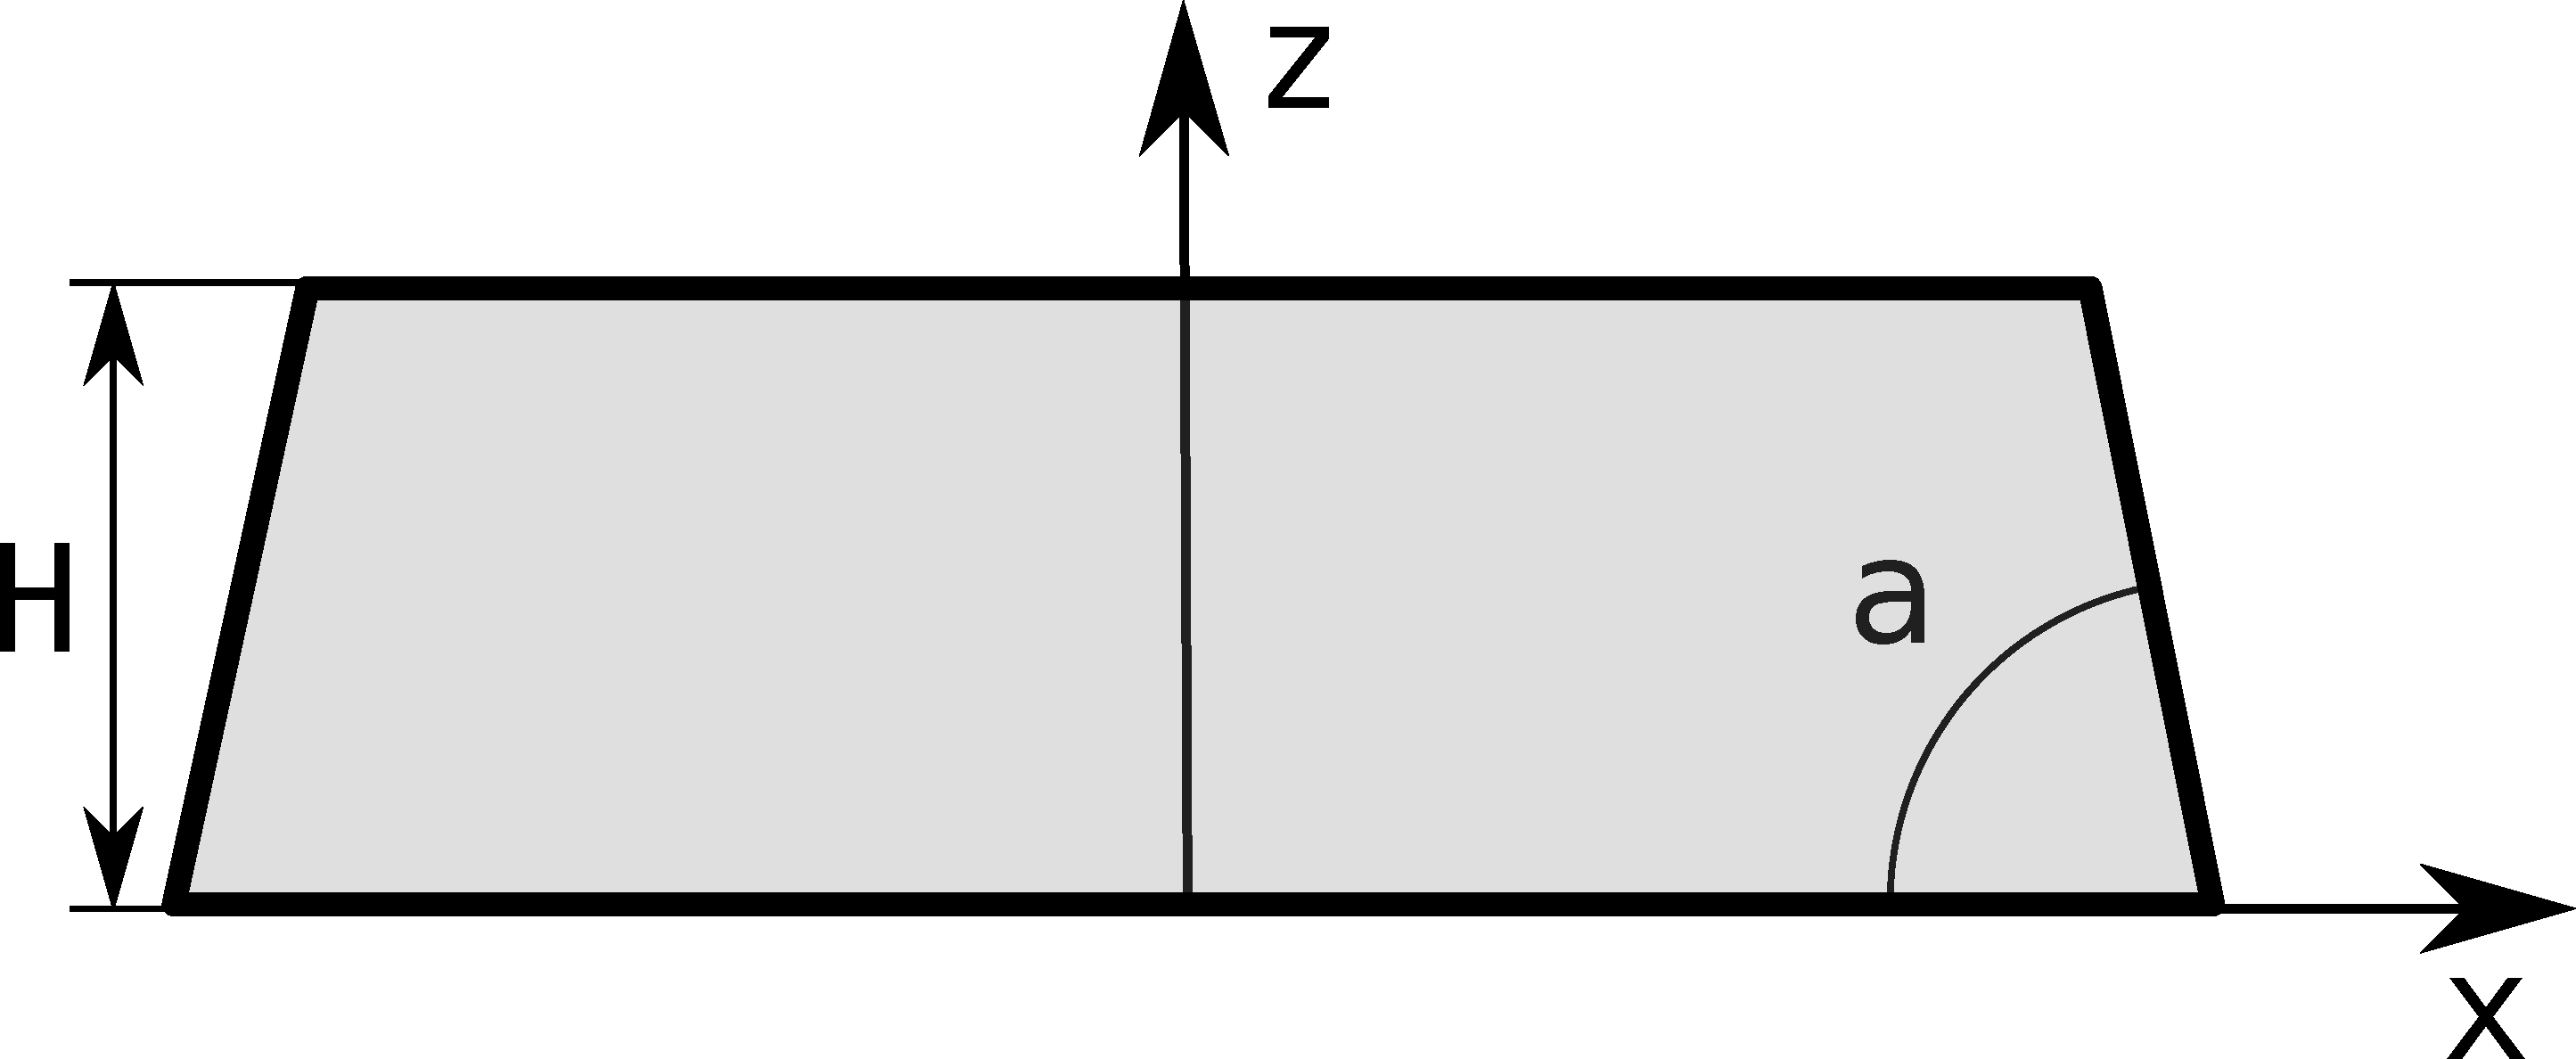
\includegraphics[width=.30\textwidth]{fig/cuts/AnisoPyramid2dxz.pdf}}}
\hfill
\caption{A truncated pyramid with a rectangular base.}
\end{figure}

\FloatBarrier

\paragraph{Syntax and parameters}\strut\\[-2ex plus .2ex minus .2ex]
\begin{lstlisting}
  FormFactorAnisoPyramid(length, width, height, alpha)
\end{lstlisting}
with the parameters
\begin{itemize}
\item \texttt{length} of the base, $L$,
\item \texttt{width} of the base, $W$,
\item \texttt{height}, $H$
\item \texttt{alpha}, angle between the base and a side face, $\alpha$.
\end{itemize}
They must fulfill
\begin{displaymath}
  H \le \frac{\tan\alpha}{2} \min\,(L,W).
\end{displaymath}

\paragraph{Form factor, volume, horizontal section}\strut\\
\begin{equation*}
  F \text{~: computed using the generic polyhedron form factor~\cite{ba:ffp},}
\end{equation*}
\begin{equation*}
  V= H \Big[LW - \dfrac{(L + W)H}{\tan\alpha} + \dfrac{4}{3} \dfrac{H^2}{\tan^2\alpha}\Big].
\end{equation*}
\begin{equation*}
  S=LW.
\end{equation*}

\paragraph{Examples}\strut\\
\begin{figure}[H]
\begin{center}
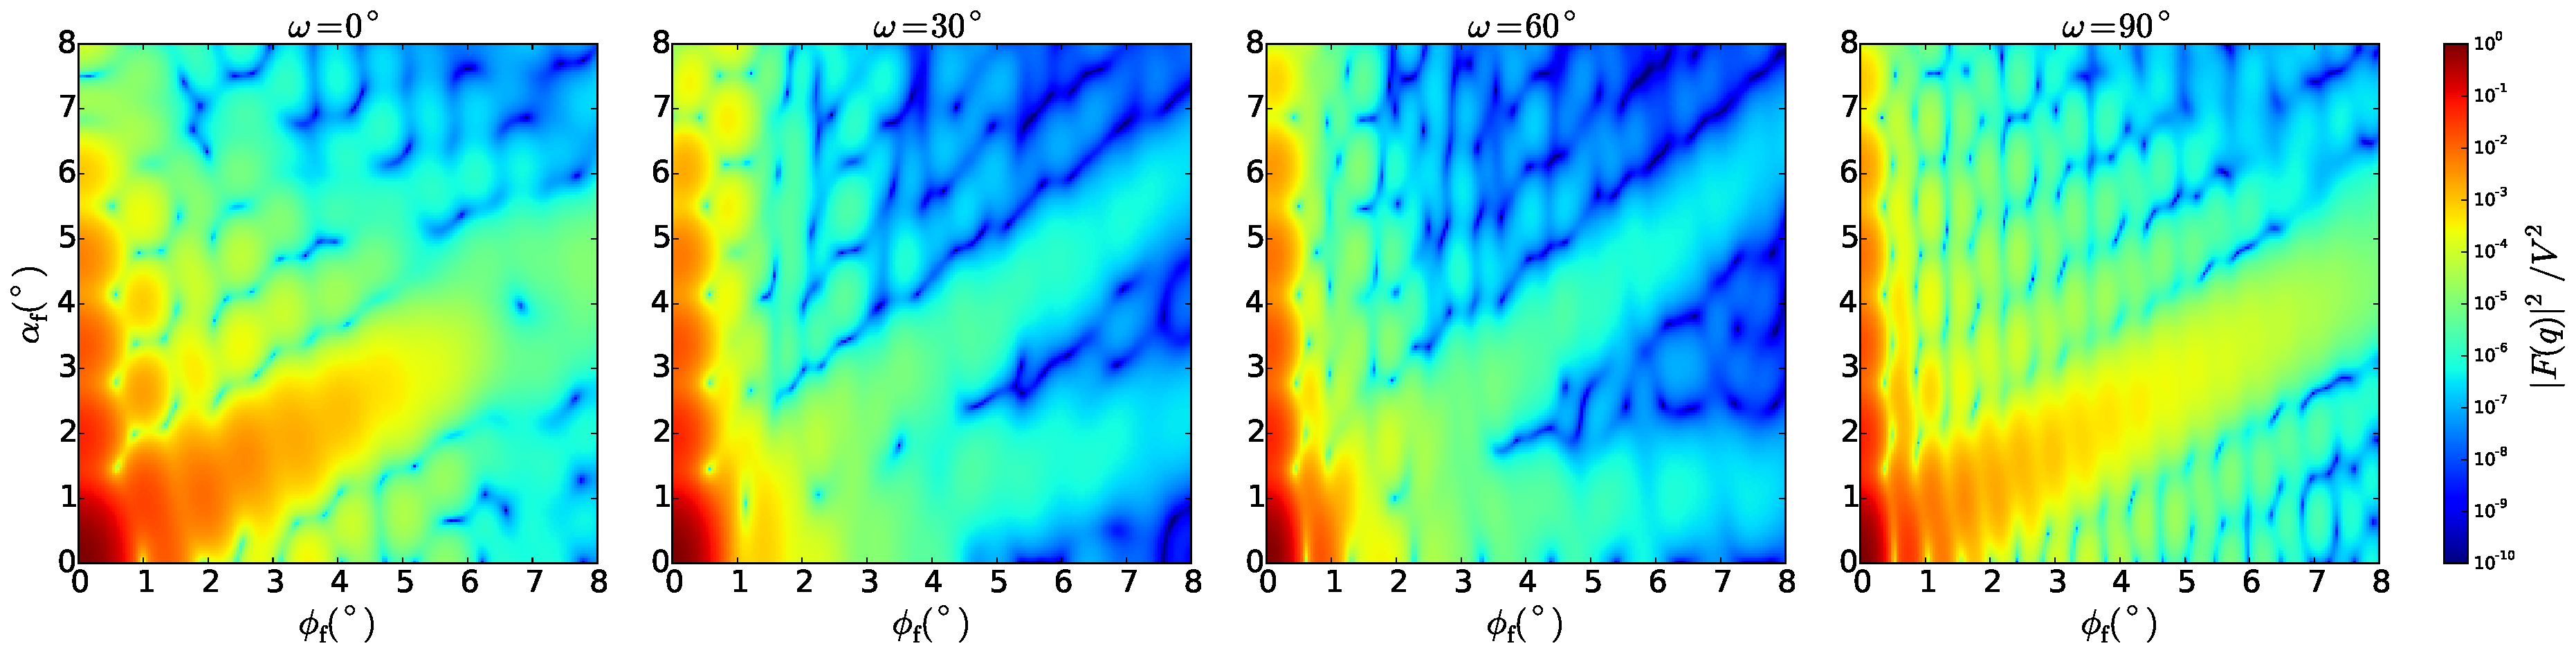
\includegraphics[width=\textwidth]{fig/ff2/ff_AnisoPyramid.pdf}
\end{center}
\caption{Normalized intensity $|F|^2/V^2$,
computed with $L=13$~nm, $W=8$~nm, $H=4.2$~nm, and $\alpha=60^\circ$,
for four different angles~$\omega$ of rotation around the $z$ axis.}
\label{fig:FFAnisoPyramidEx}
\end{figure}

\paragraph{History}\strut\\
Agrees with the \E{In-plane anisotropic pyramid} form factor of \IsGISAXS\
\cite[Eq.~2.40]{Laz08} \cite[Eq.~217]{ReLL09},
except for different parametrization.
This is \E{not} the \E{anisotropic pyramid} of \FitGISAXS,
which is a true pyramid with an off-center apex \cite{Bab13}.

Formfactors~$F(\q)$ have been checked against the different computation of \IsGISAXS,
and were found to fully agree.

%===============================================================================
\ffsection{Box (cuboid)} \label{SBox}
%===============================================================================
  \index{Box (form factor)}
  \index{Cuboid (form factor)}
  \index{Prism (form factor)!reactangular (Box)}
  \index{Platonic solids!cube}
  \index{FormFactorBox@\Code{FormFactorBox}}

\paragraph{Real-space geometry}\strut\\

\begin{figure}[H]
\hfill
\subfigure[Perspective]{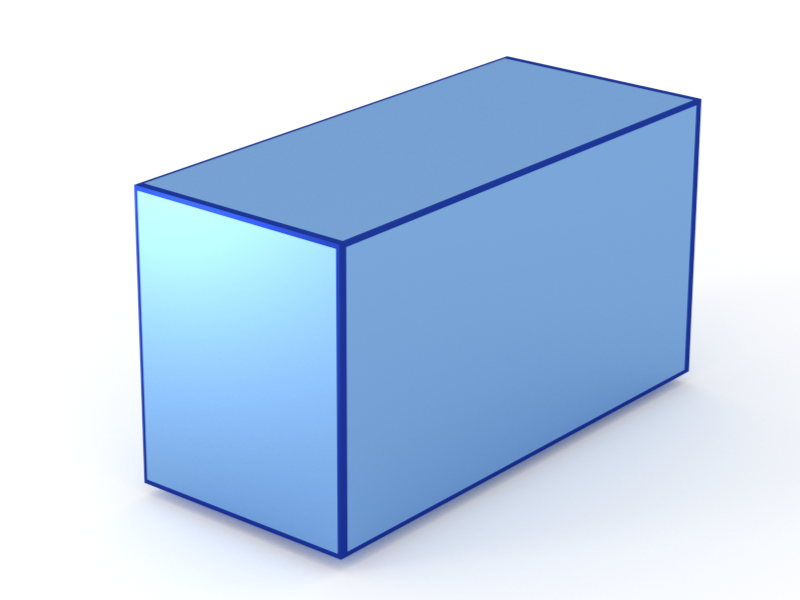
\includegraphics[width=.24\textwidth]{fig/blue/Box3d.png}}
\hfill
\subfigure[Top view]{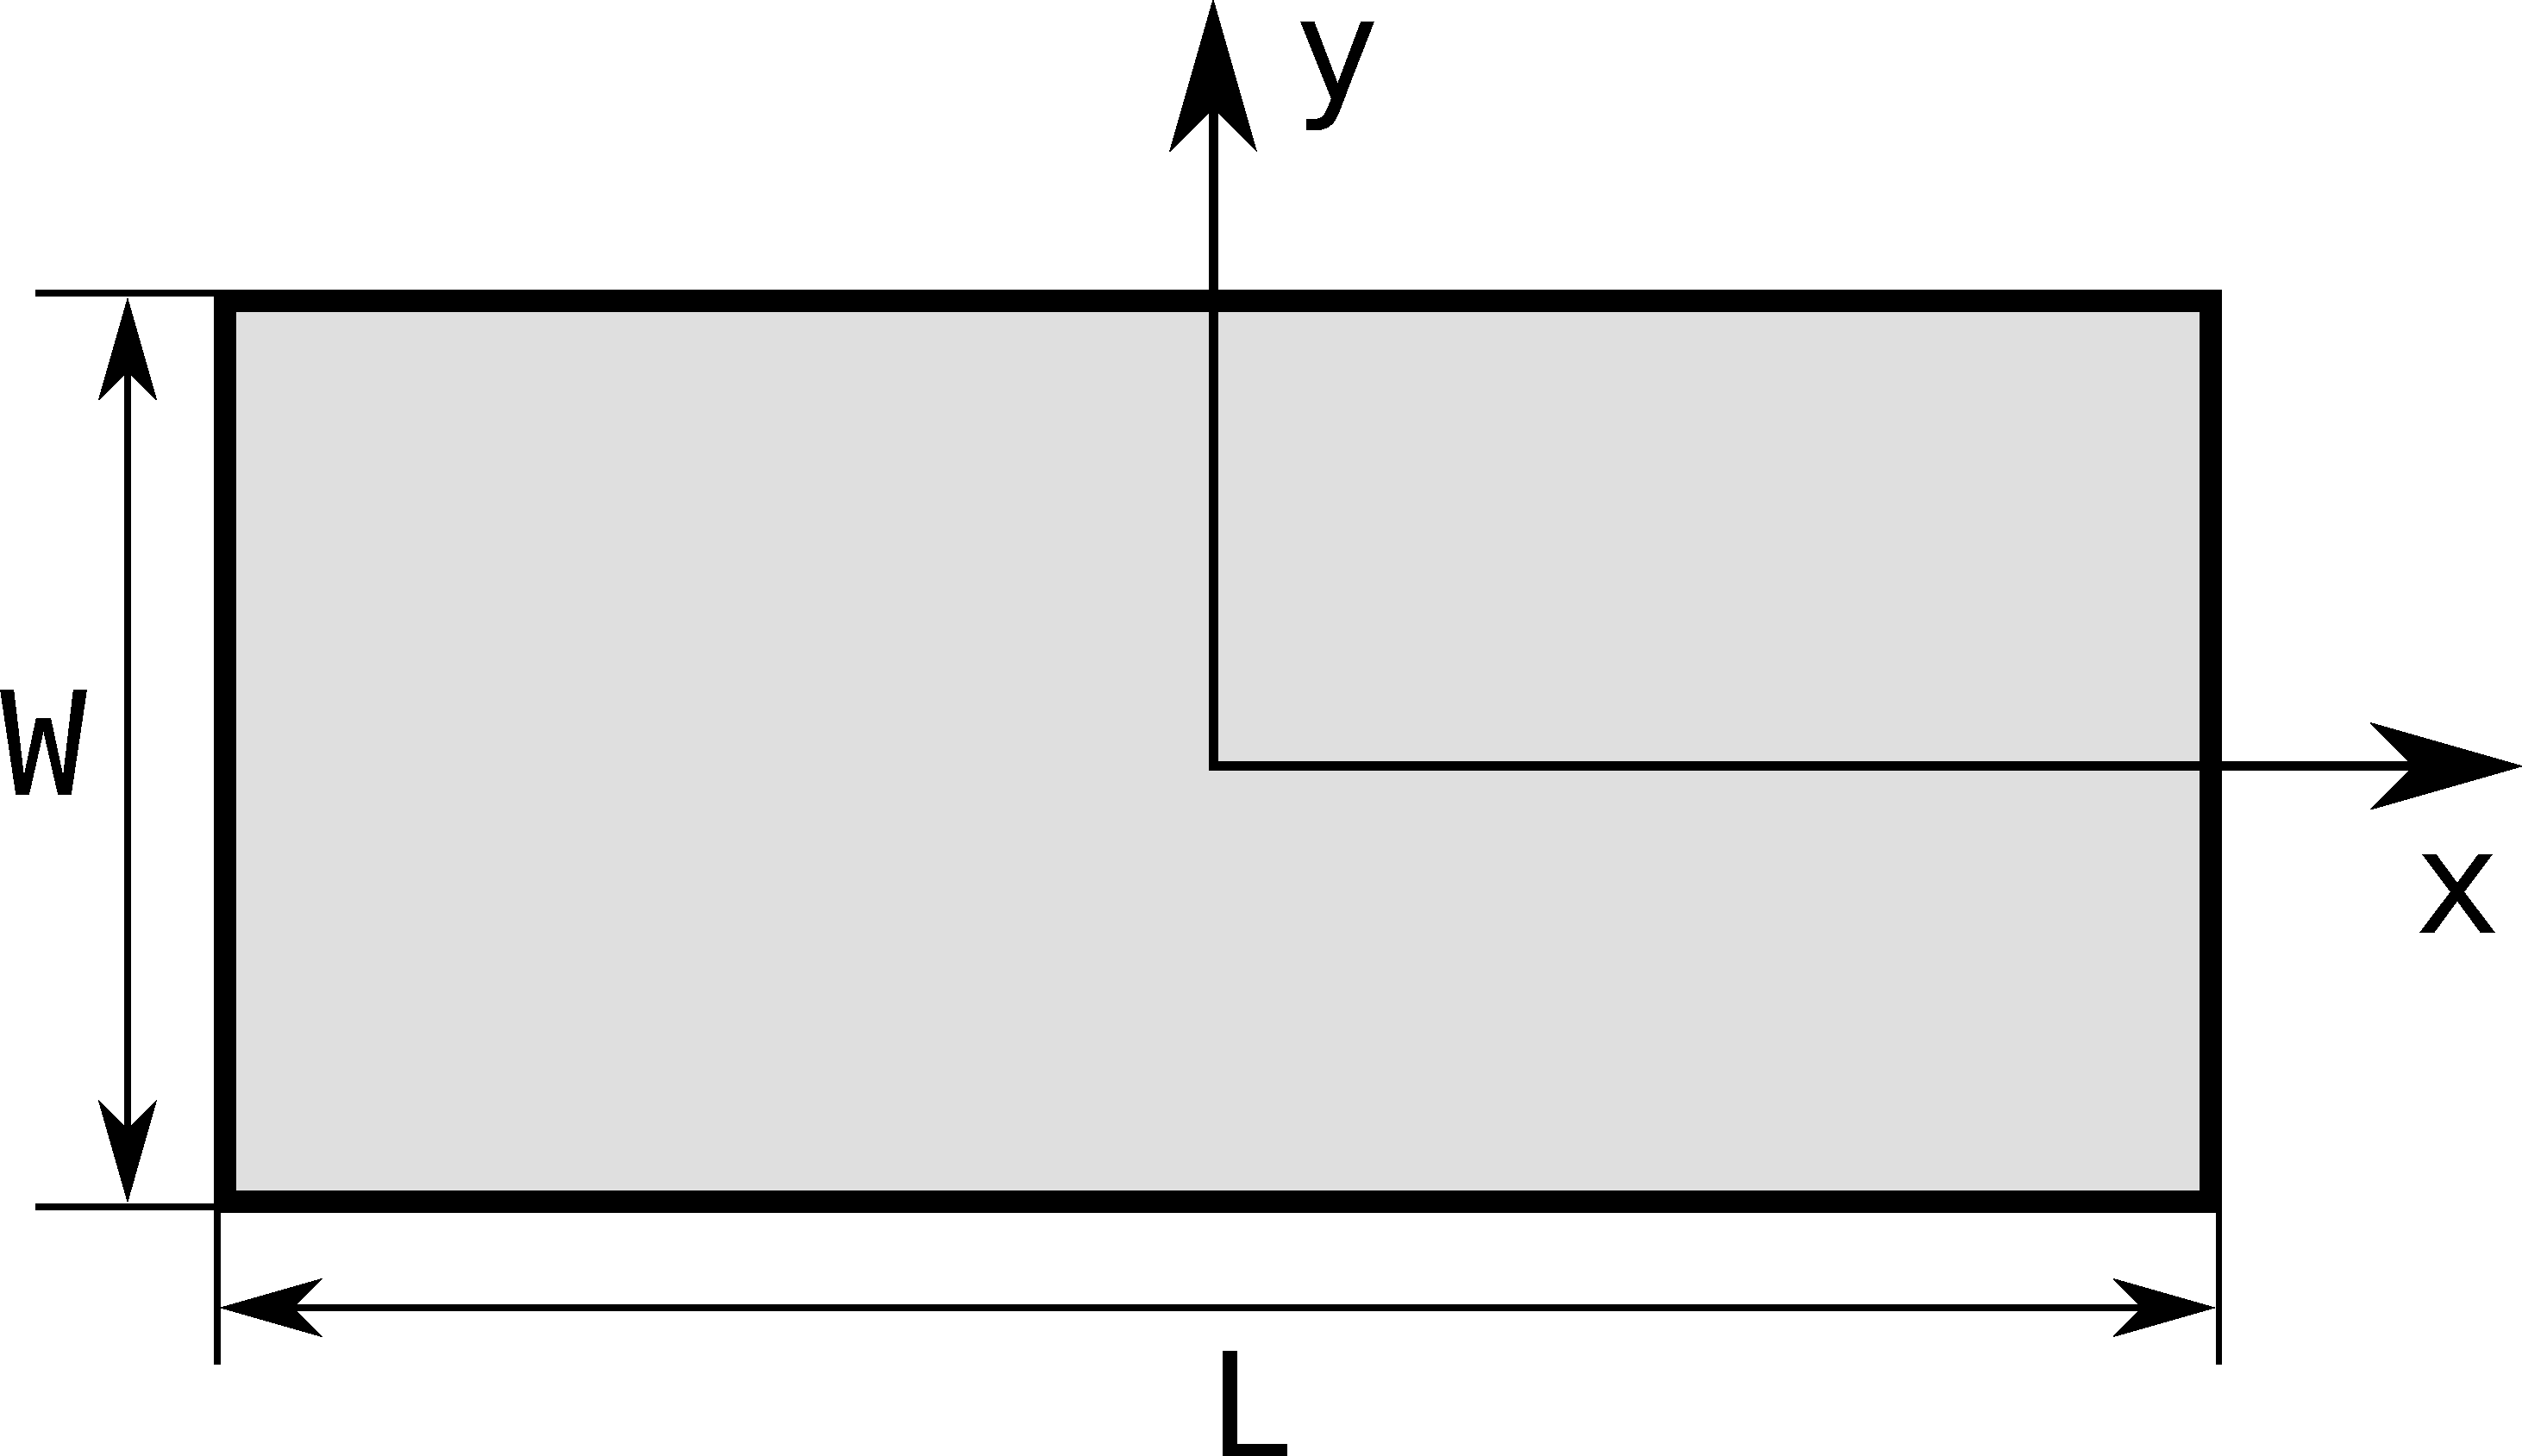
\includegraphics[width=.30\textwidth]{fig/cuts/Box2dxy.pdf}}
\hfill
\subfigure[Side view]{\raisebox{2mm}{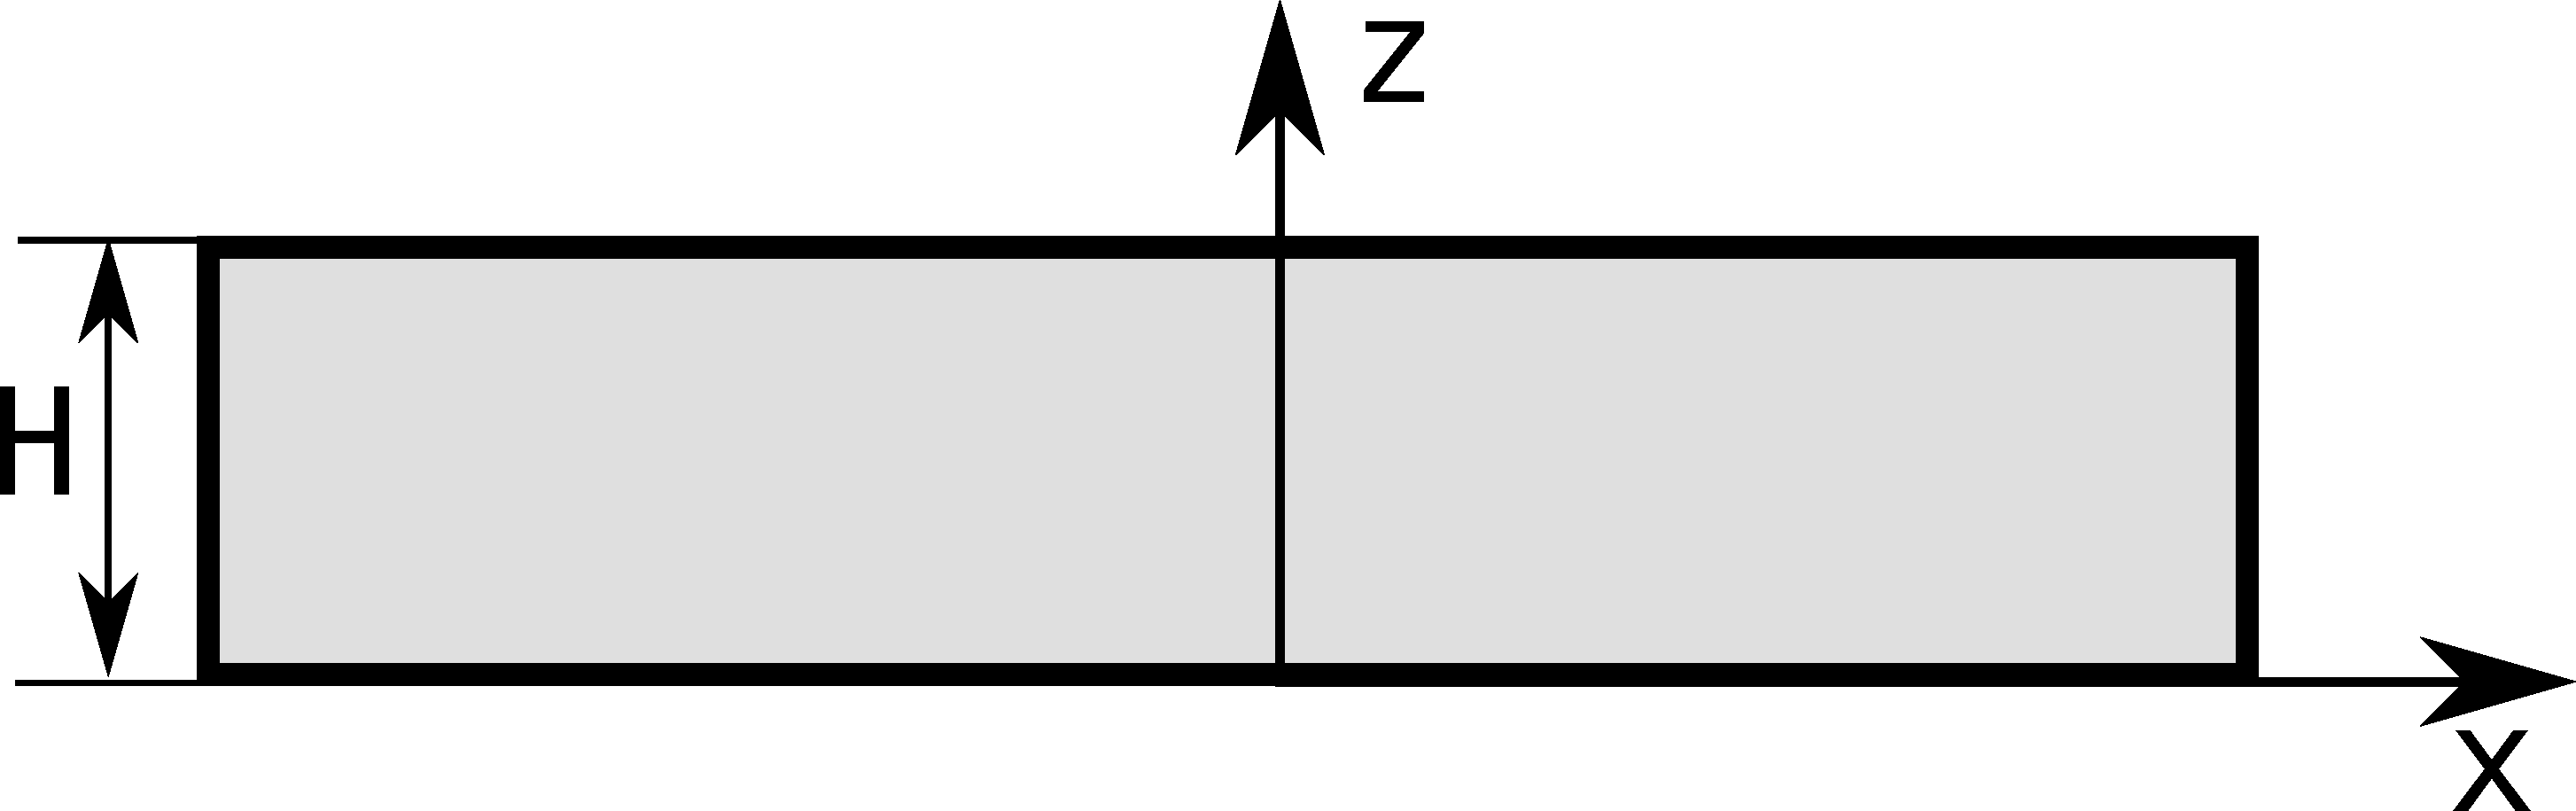
\includegraphics[width=.30\textwidth]{fig/cuts/Box2dxz.pdf}}}
\hfill
\caption{A rectangular cuboid.}
\end{figure}

\FloatBarrier

\paragraph{Syntax and parameters}\strut\\[-2ex plus .2ex minus .2ex]
\begin{lstlisting}
  FormFactorBox(length, width, height)
\end{lstlisting}
with the parameters
\begin{itemize}
\item \texttt{length} of the base, $L$,
\item \texttt{width} of the base, $W$,
\item \texttt{height}, $H$.
\end{itemize}

\paragraph{Form factor, volume, horizontal section}

\begin{equation*}
F= L W H\exp\left(i q_z \frac{H}{2}\right) \sinc\left(q_x \frac{L}{2}\right)
\sinc\left(q_y \frac{W}{2}\right) \sinc\left(q_z \frac{H}{2}\right),
\end{equation*}
\begin{equation*}
  V= LWH,
\end{equation*}
\begin{equation*}
  S = LW.
\end{equation*}

\paragraph{Examples}\strut

\begin{figure}[H]
\begin{center}
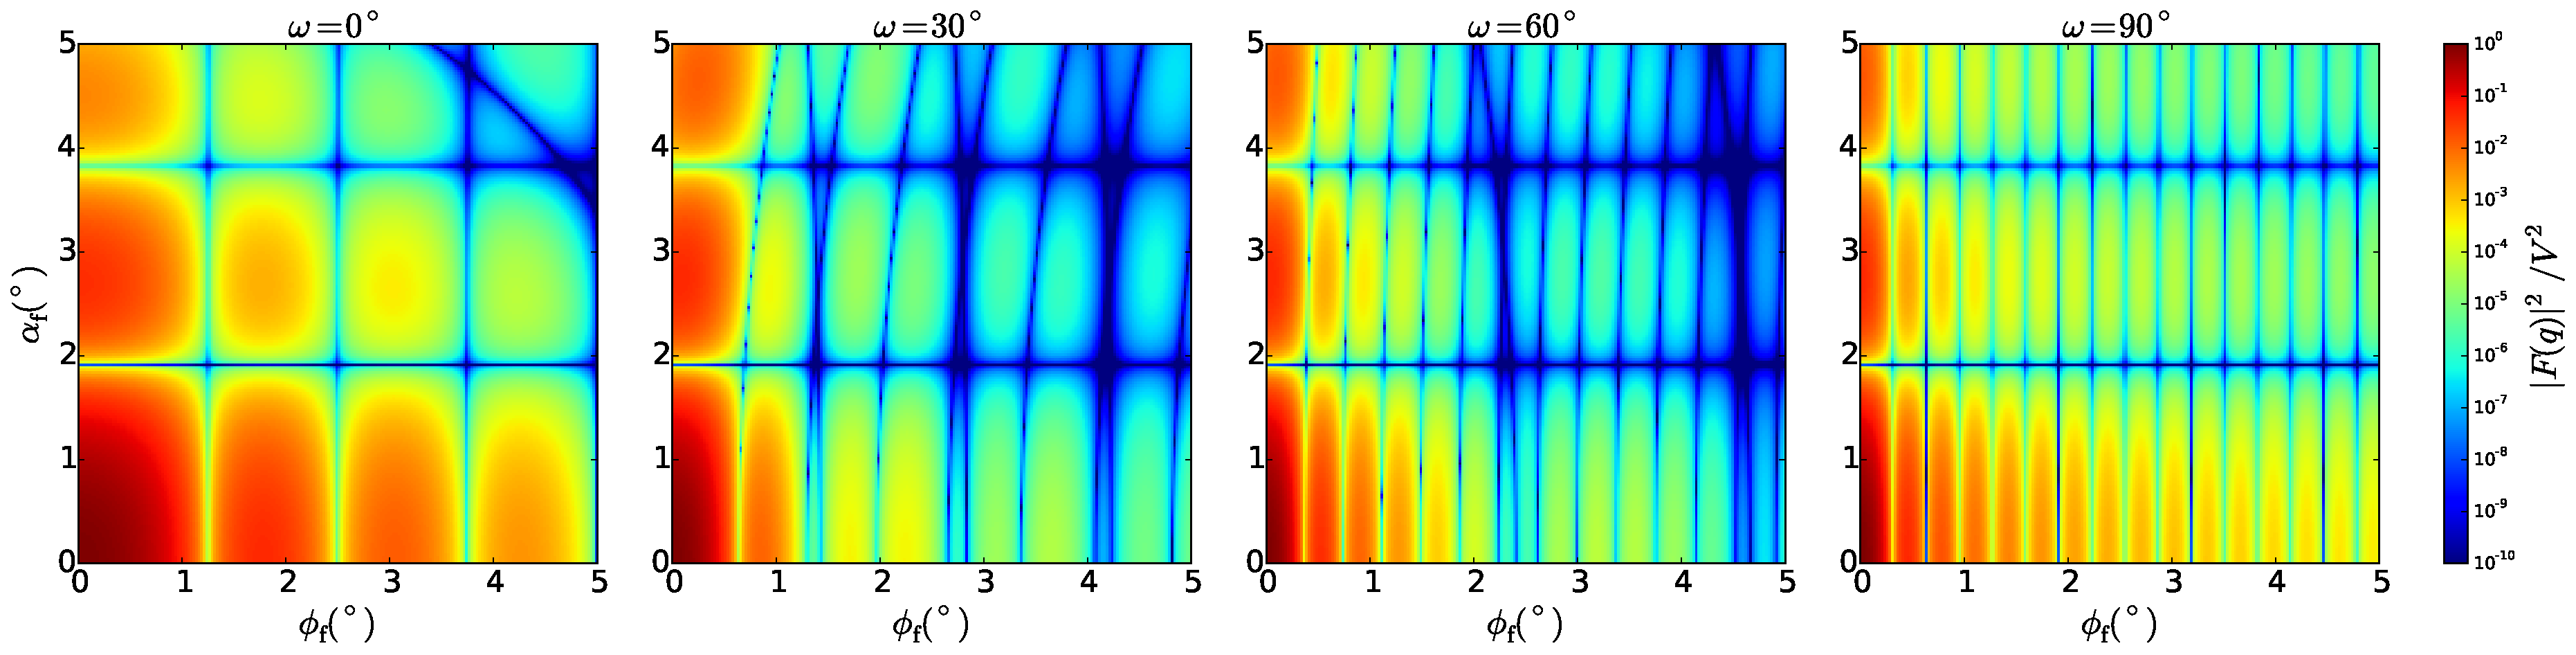
\includegraphics[width=\textwidth]{fig/ff2/ff_Box.pdf}
\end{center}
\caption{Normalized intensity $|F|^2/V^2$,
computed with $L=18$~nm, $W=4.6$~nm, and $H=3$~nm,
for four different angles~$\omega$ of rotation around the $z$ axis.}
\end{figure}

\paragraph{History}\strut\\
Agrees with \E{Box} form factor of \IsGISAXS\
\cite[Eq.~2.38]{Laz08} \cite[Eq.~214]{ReLL09},
except for factors $1/2$ in the definitions of parameters $L$, $W$, $H$.


%===============================================================================
\ffsection{Cone (circular)} \label{SCone}
%===============================================================================
  \index{Cone (form factor)!circular}
  \index{Truncated cone (form factor)}
  \index{FormFactorCone@\Code{FormFactorCone}}

\paragraph{Real-space geometry}\strut\\

\begin{figure}[H]
\hfill
\subfigure[Perspective]{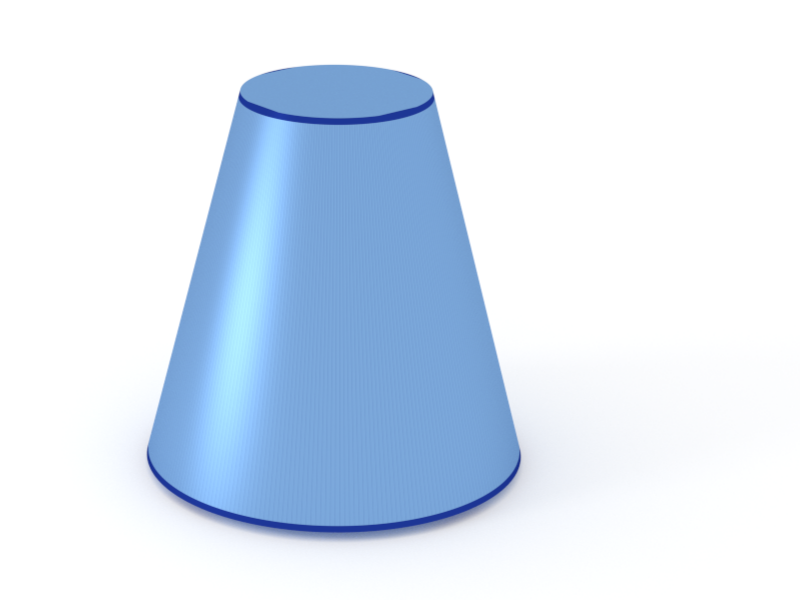
\includegraphics[width=.24\textwidth]{fig/blue/Cone3d.png}}
\hfill
\subfigure[Top view]{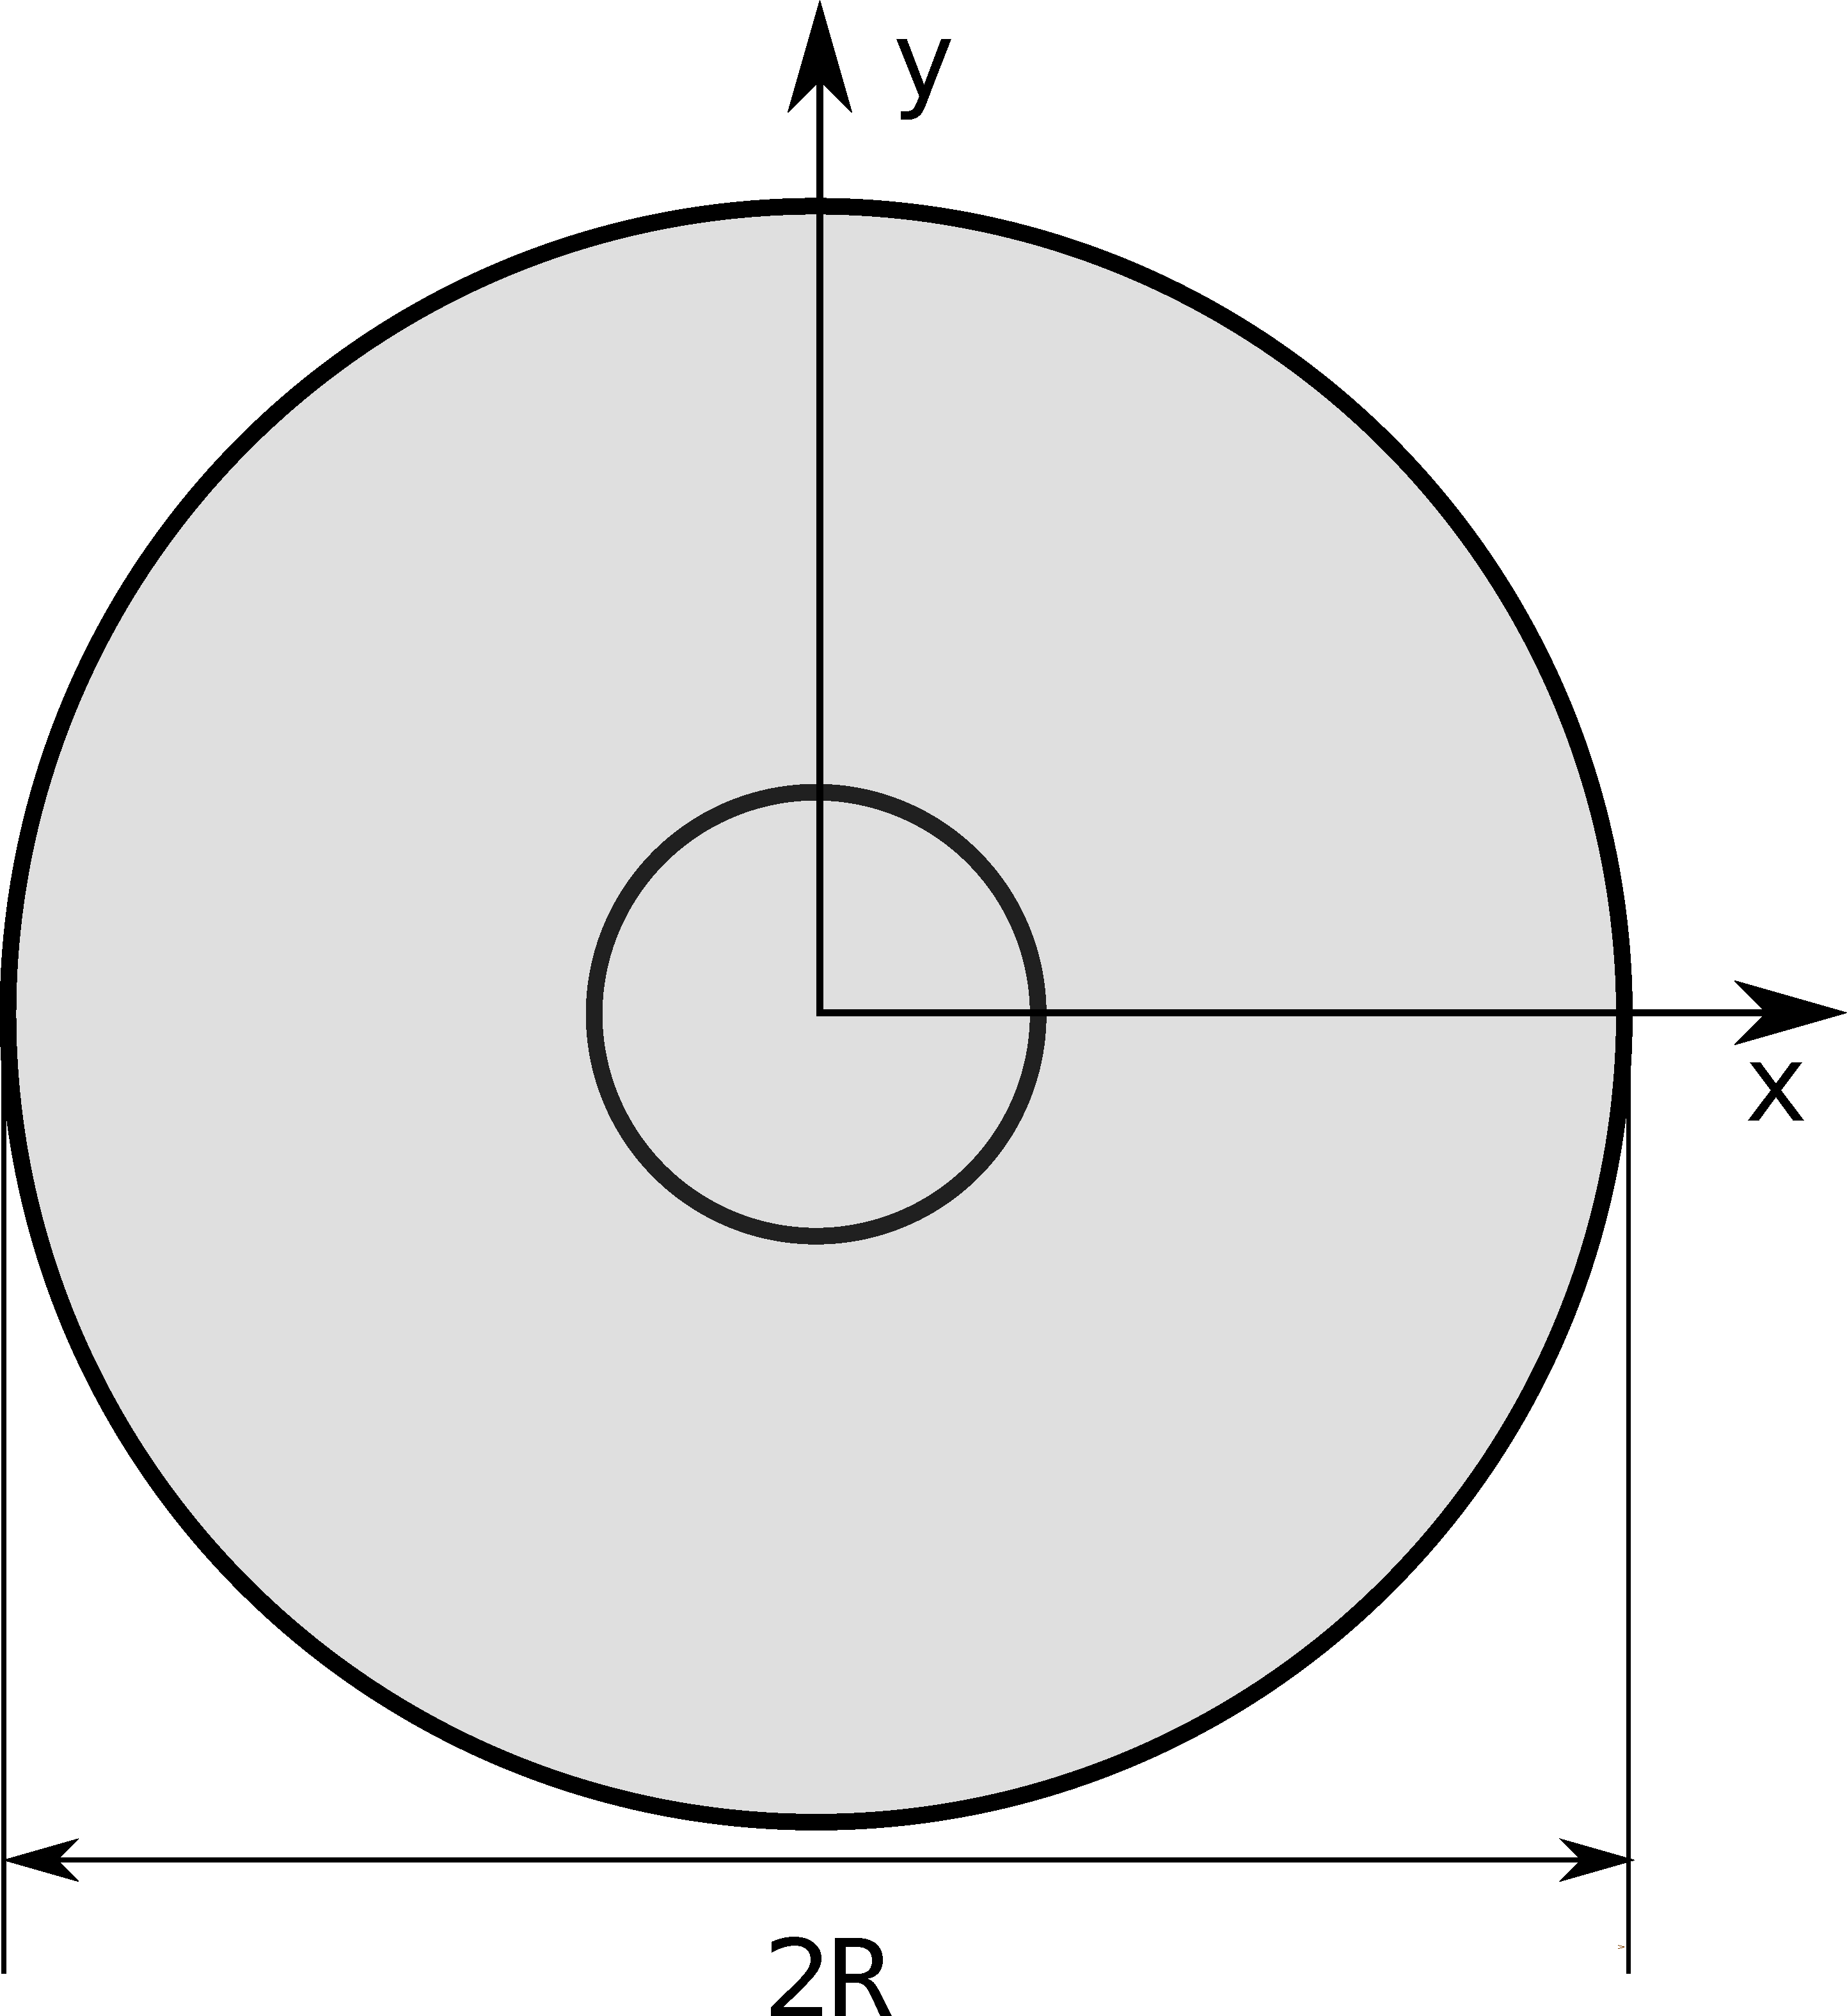
\includegraphics[width=.30\textwidth]{fig/cuts/Cone2dxy.pdf}}
\hfill
\subfigure[Side view]{\raisebox{3mm}{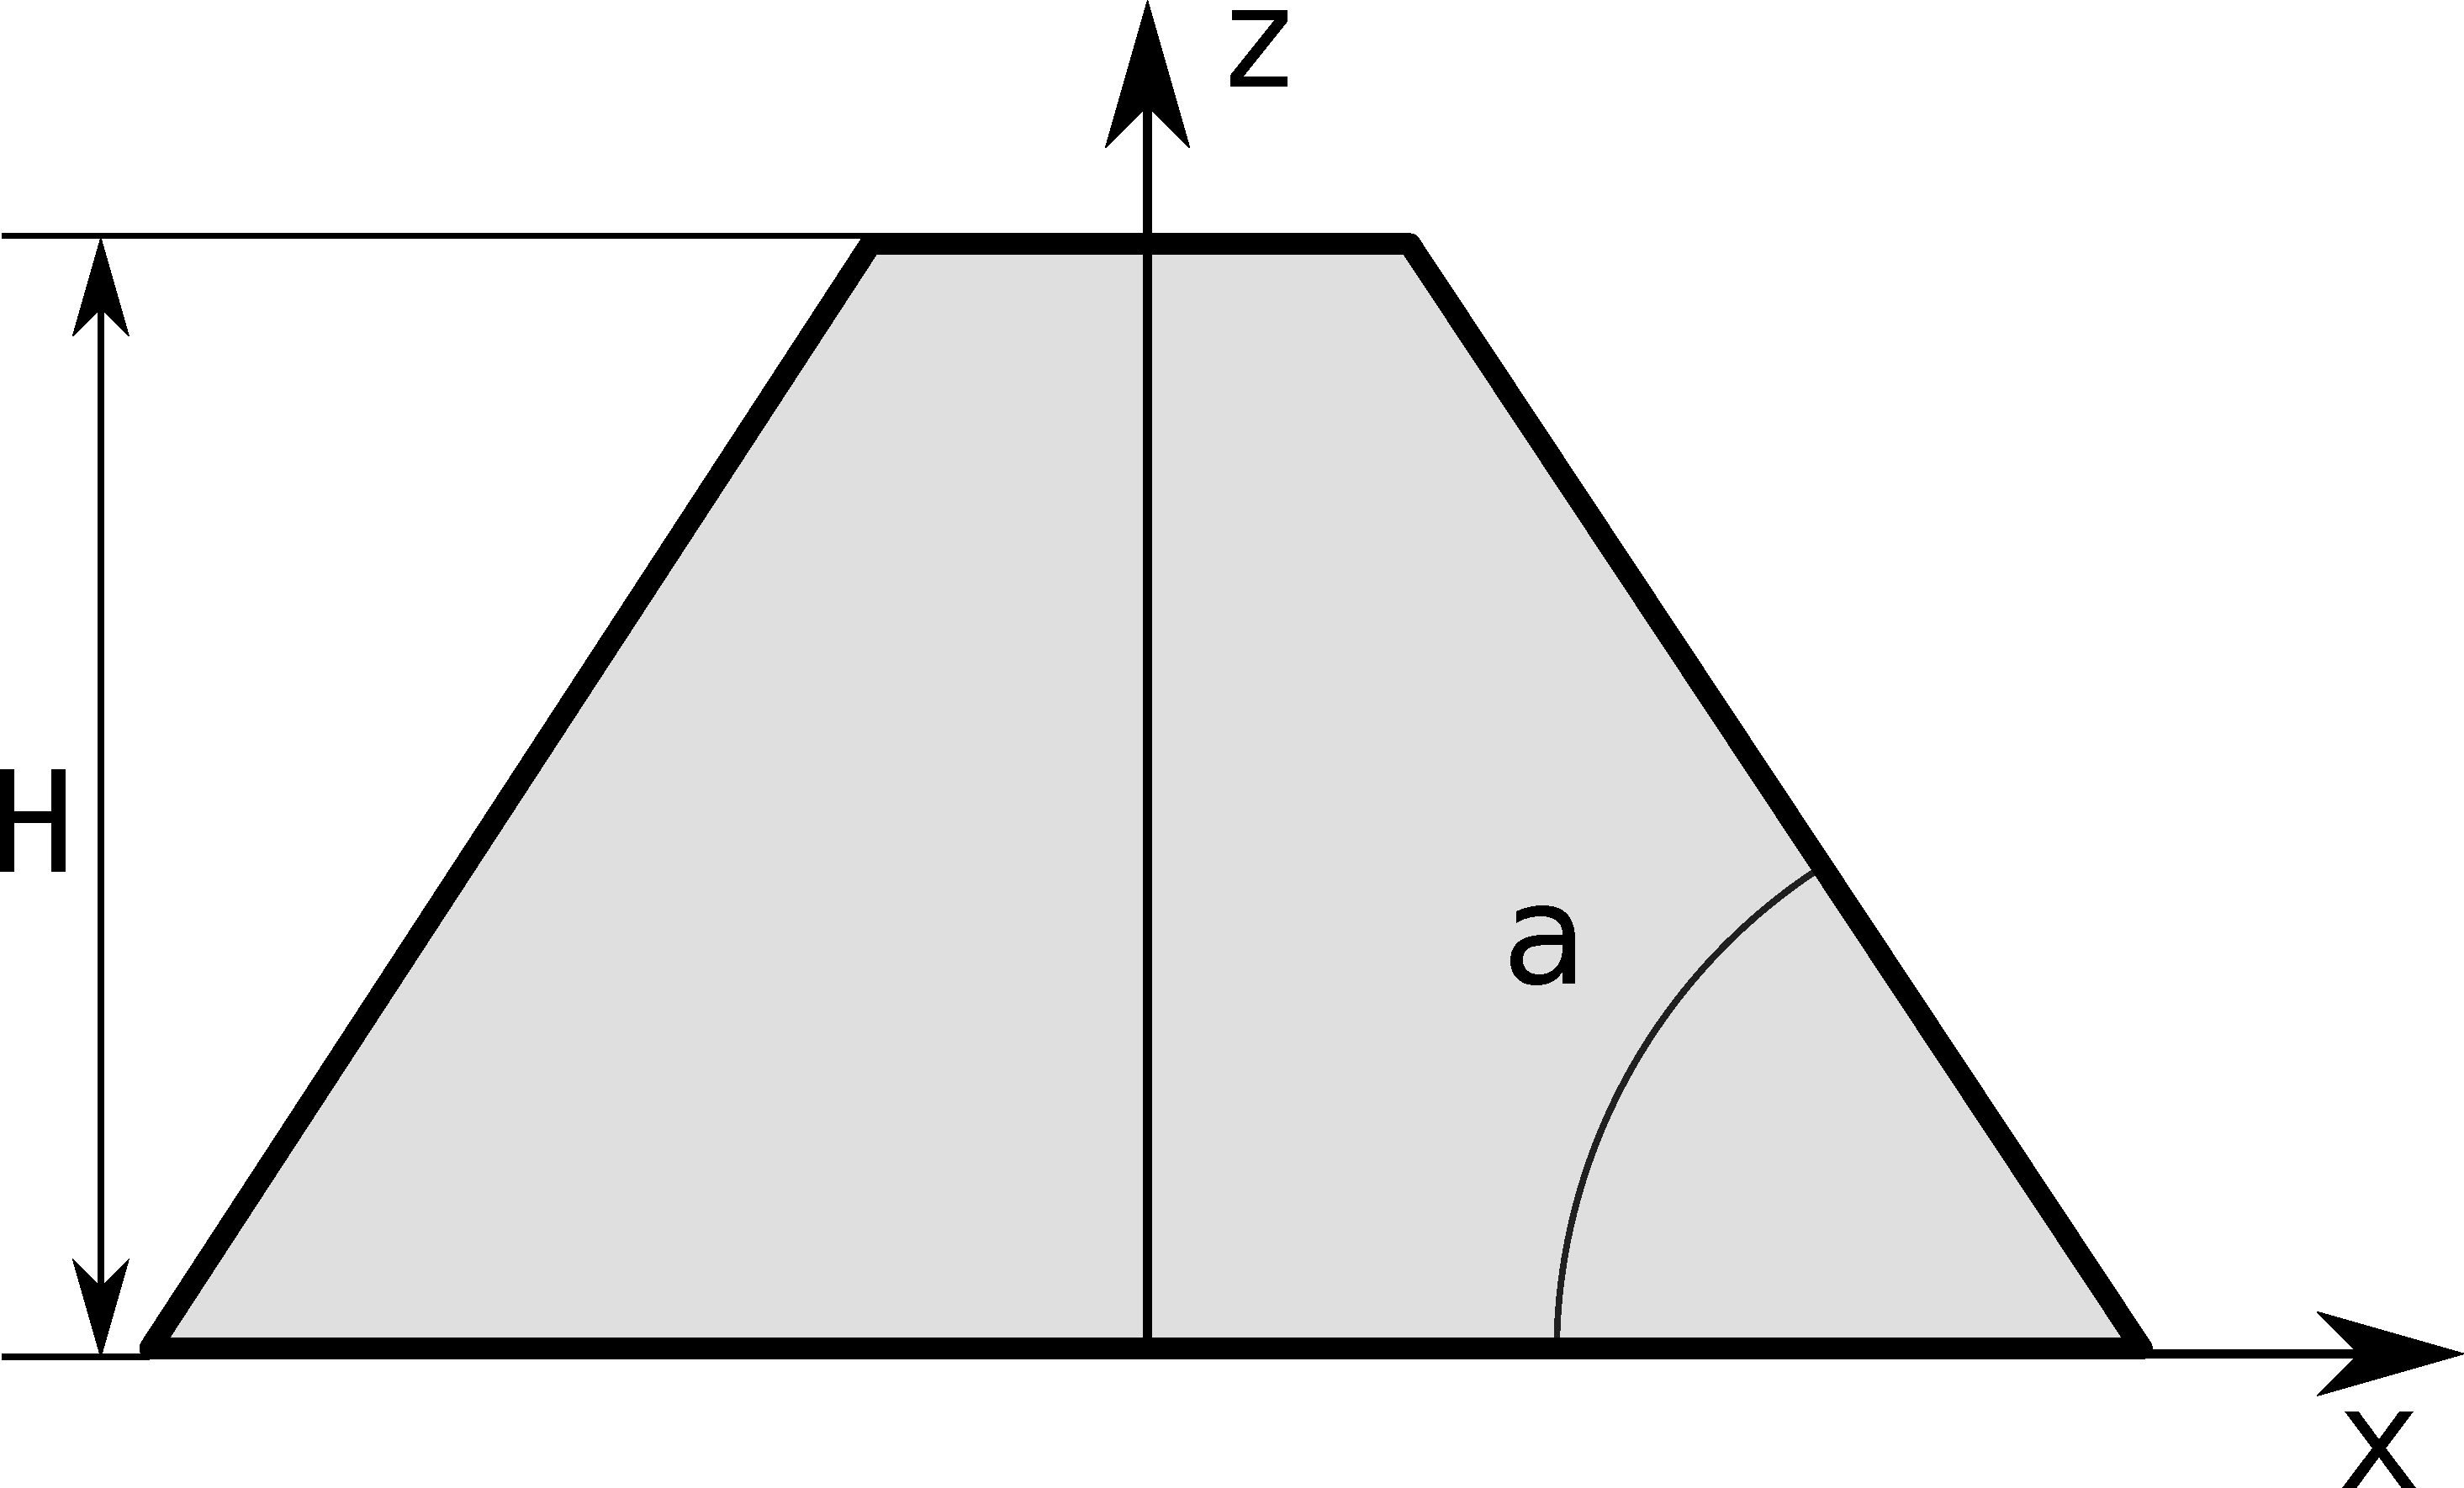
\includegraphics[width=.30\textwidth]{fig/cuts/Cone2dxz.pdf}}}
\hfill
\caption{A truncated cone with circular base.}
\end{figure}

\paragraph{Syntax and parameters}\strut\\[-2ex plus .2ex minus .2ex]
\begin{lstlisting}
  FormFactorCone(radius, height, alpha)
\end{lstlisting}
with the parameters
\begin{itemize}
\item \texttt{radius}, $R$,
\item \texttt{height}, $H$,
\item \texttt{alpha}, angle between the side and the base, $\alpha$.
\end{itemize}
They must fulfill
\begin{displaymath}
  H\le R\tan\alpha.
\end{displaymath}

\paragraph{Form factor, volume, horizontal section}\strut\\
Notation:
\begin{equation*}
  R_H \coloneqq R-\dfrac{H}{\tan \alpha}, \quad
  q_{\parallel} \coloneqq \sqrt{q_x^2+ q_y^2}, \quad
  \tilde{q}_z \coloneqq q_z \tan\alpha.
\end{equation*}
Results:
\begin{equation*}
  F = 2\pi \tan\alpha\; \e^{i\tilde{q}_z R}
      \int_{R_H}^R \!\d\rho\, \rho^2
        \frac{J_1(q_{\parallel}\rho)}{q_{\parallel}\rho}\,\e^{-i\tilde{q}_z \rho},
\end{equation*}
\begin{equation*}
  V = \dfrac{\pi}{3}\tan\alpha  \left( R^3 - R_H^3\right),
\end{equation*}
\begin{equation*}
  S=\pi R^2.
\end{equation*}

\paragraph{Examples}\strut

\begin{figure}[H]
\begin{center}
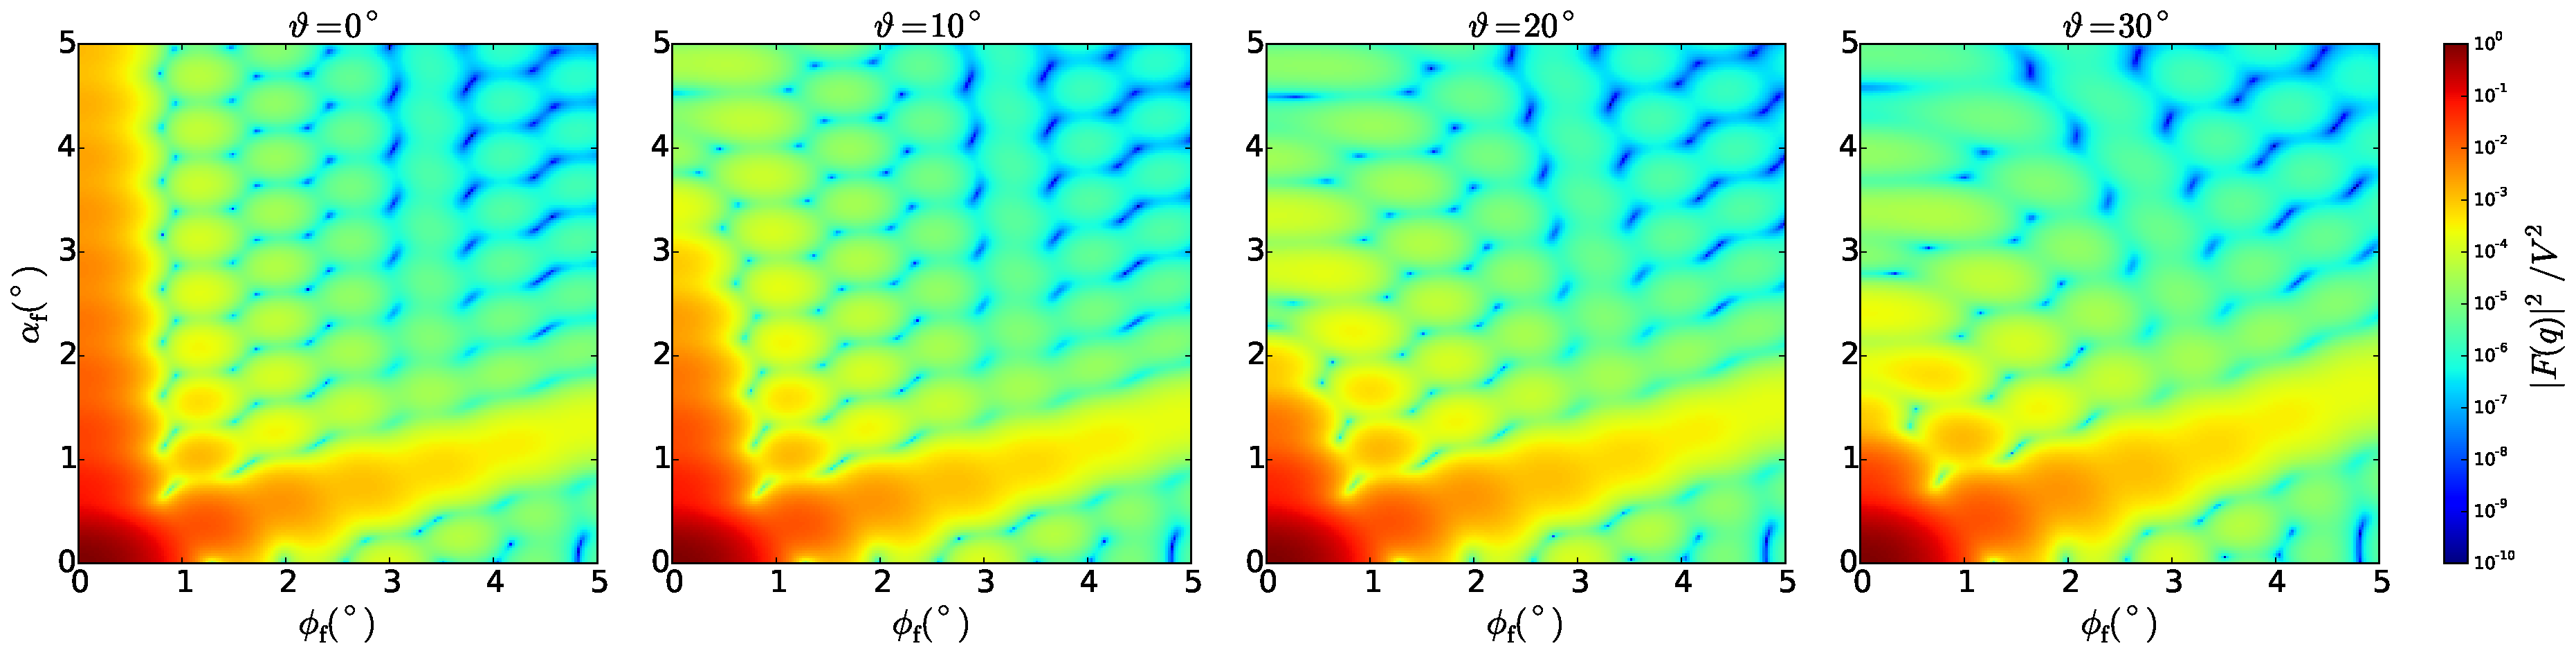
\includegraphics[width=\textwidth]{fig/ff2/ff_Cone.pdf}
\end{center}
\caption{Normalized intensity $|F|^2/V^2$,
computed with $R=4$~nm, $H=11$~nm, and $\alpha=75^\circ$,
for four different tilt angles~$\vartheta$ (rotation around the $y$ axis).}
\end{figure}

\paragraph{History}\strut\\
Agrees with \E{Cone} form factor of \IsGISAXS\
\cite[Eq.~2.28]{Laz08} \cite[Eq.~225]{ReLL09},
except for a substitution $z\to\rho$ in our expression for~$F$.


%===============================================================================
\ffsection{Cone6 (hexagonal)} \label{SCone6}
%===============================================================================
  \index{Cone (form factor)!hexagonal (Cone6)}
  \index{Pyramid (form factor)!hexagonal (Cone6)}
  \index{Truncated pyramid (form factor)!hexagonal (Cone6)}
  \index{FormFactorCone6@\Code{FormFactorCone6}}

\paragraph{Real-space geometry}\strut\\

\begin{figure}[H]
\hfill
\subfigure[Perspective]{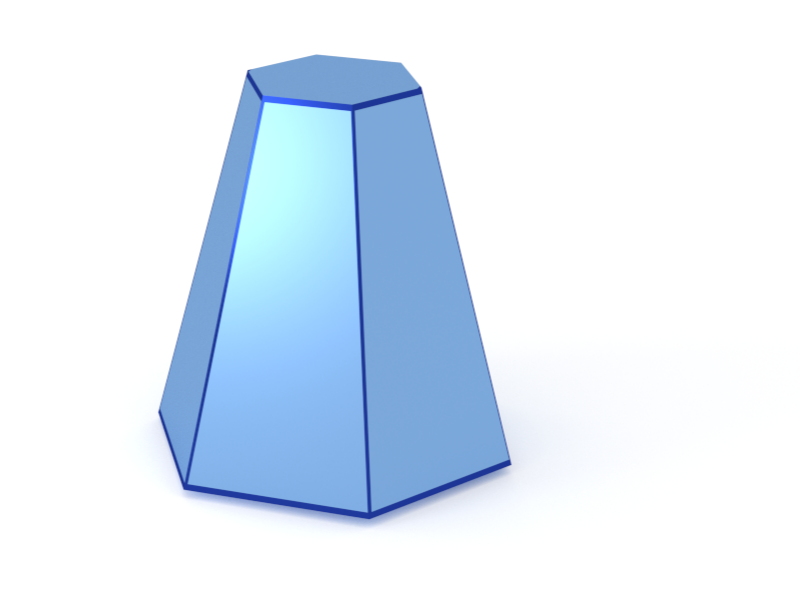
\includegraphics[width=.24\textwidth]{fig/blue/Cone63d.png}}
\hfill
\subfigure[Top view]{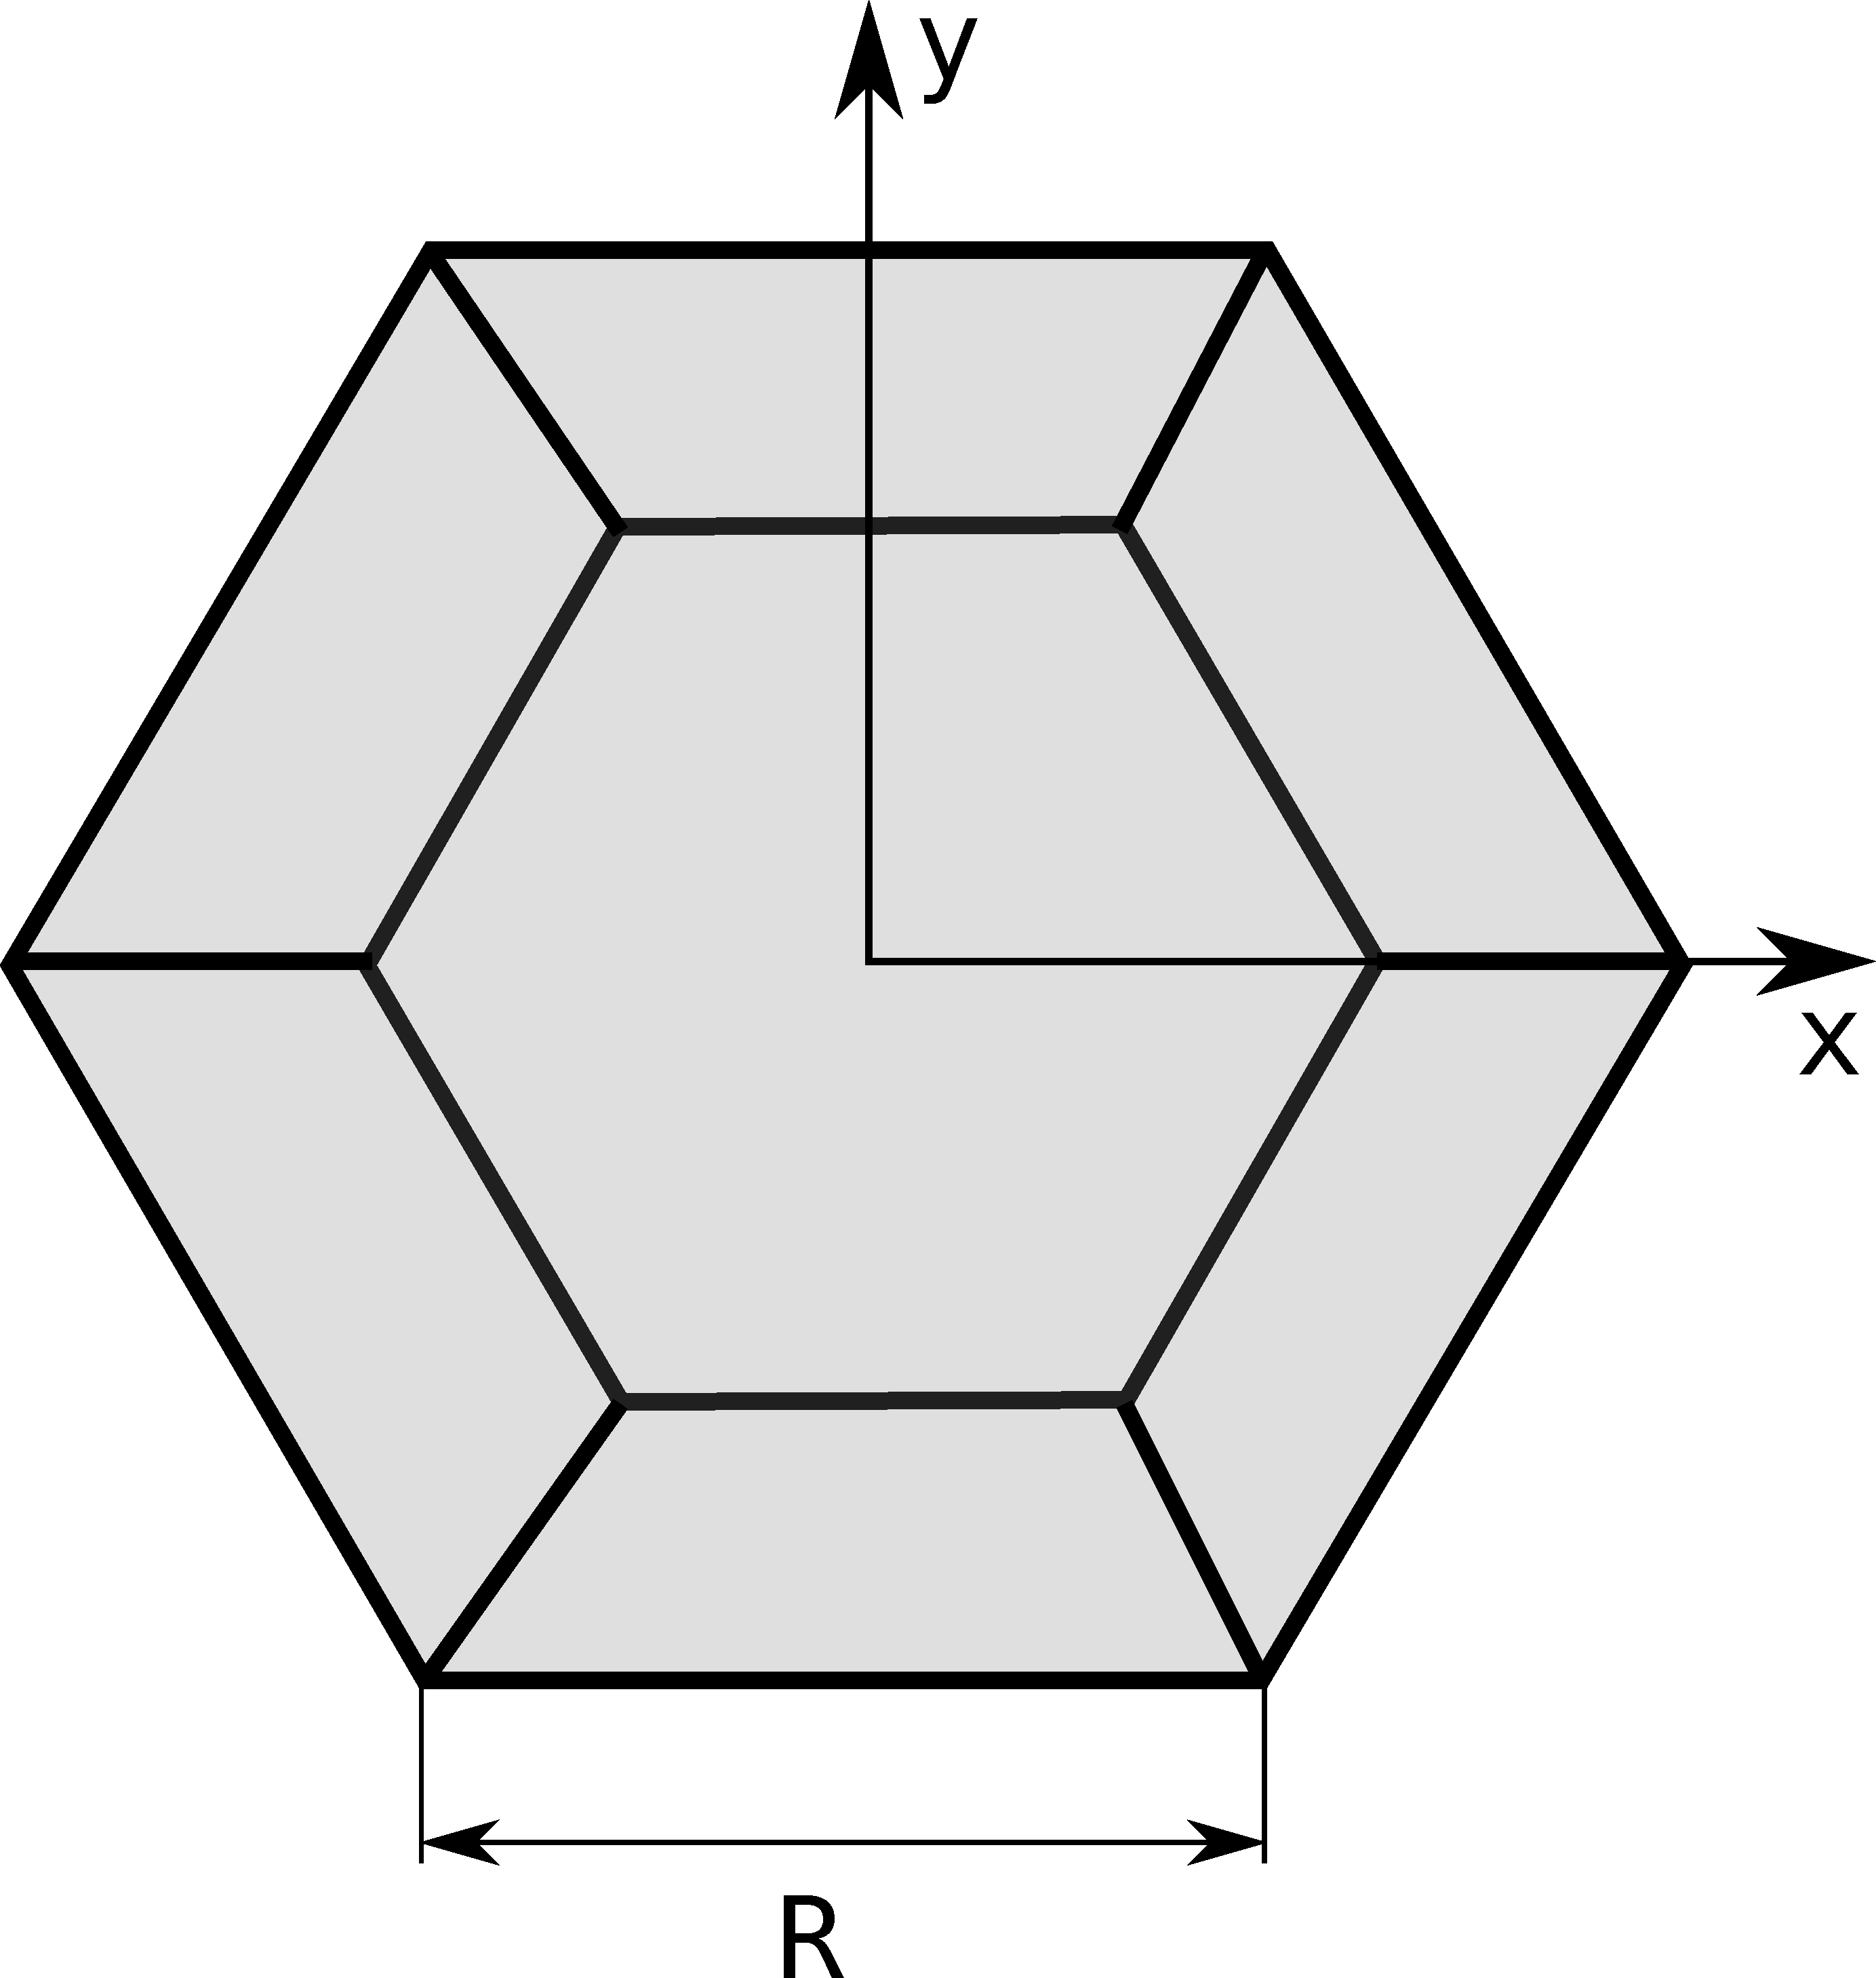
\includegraphics[width=.30\textwidth]{fig/cuts/Cone62dxy.pdf}}
\hfill
\subfigure[Side view]{\raisebox{5mm}{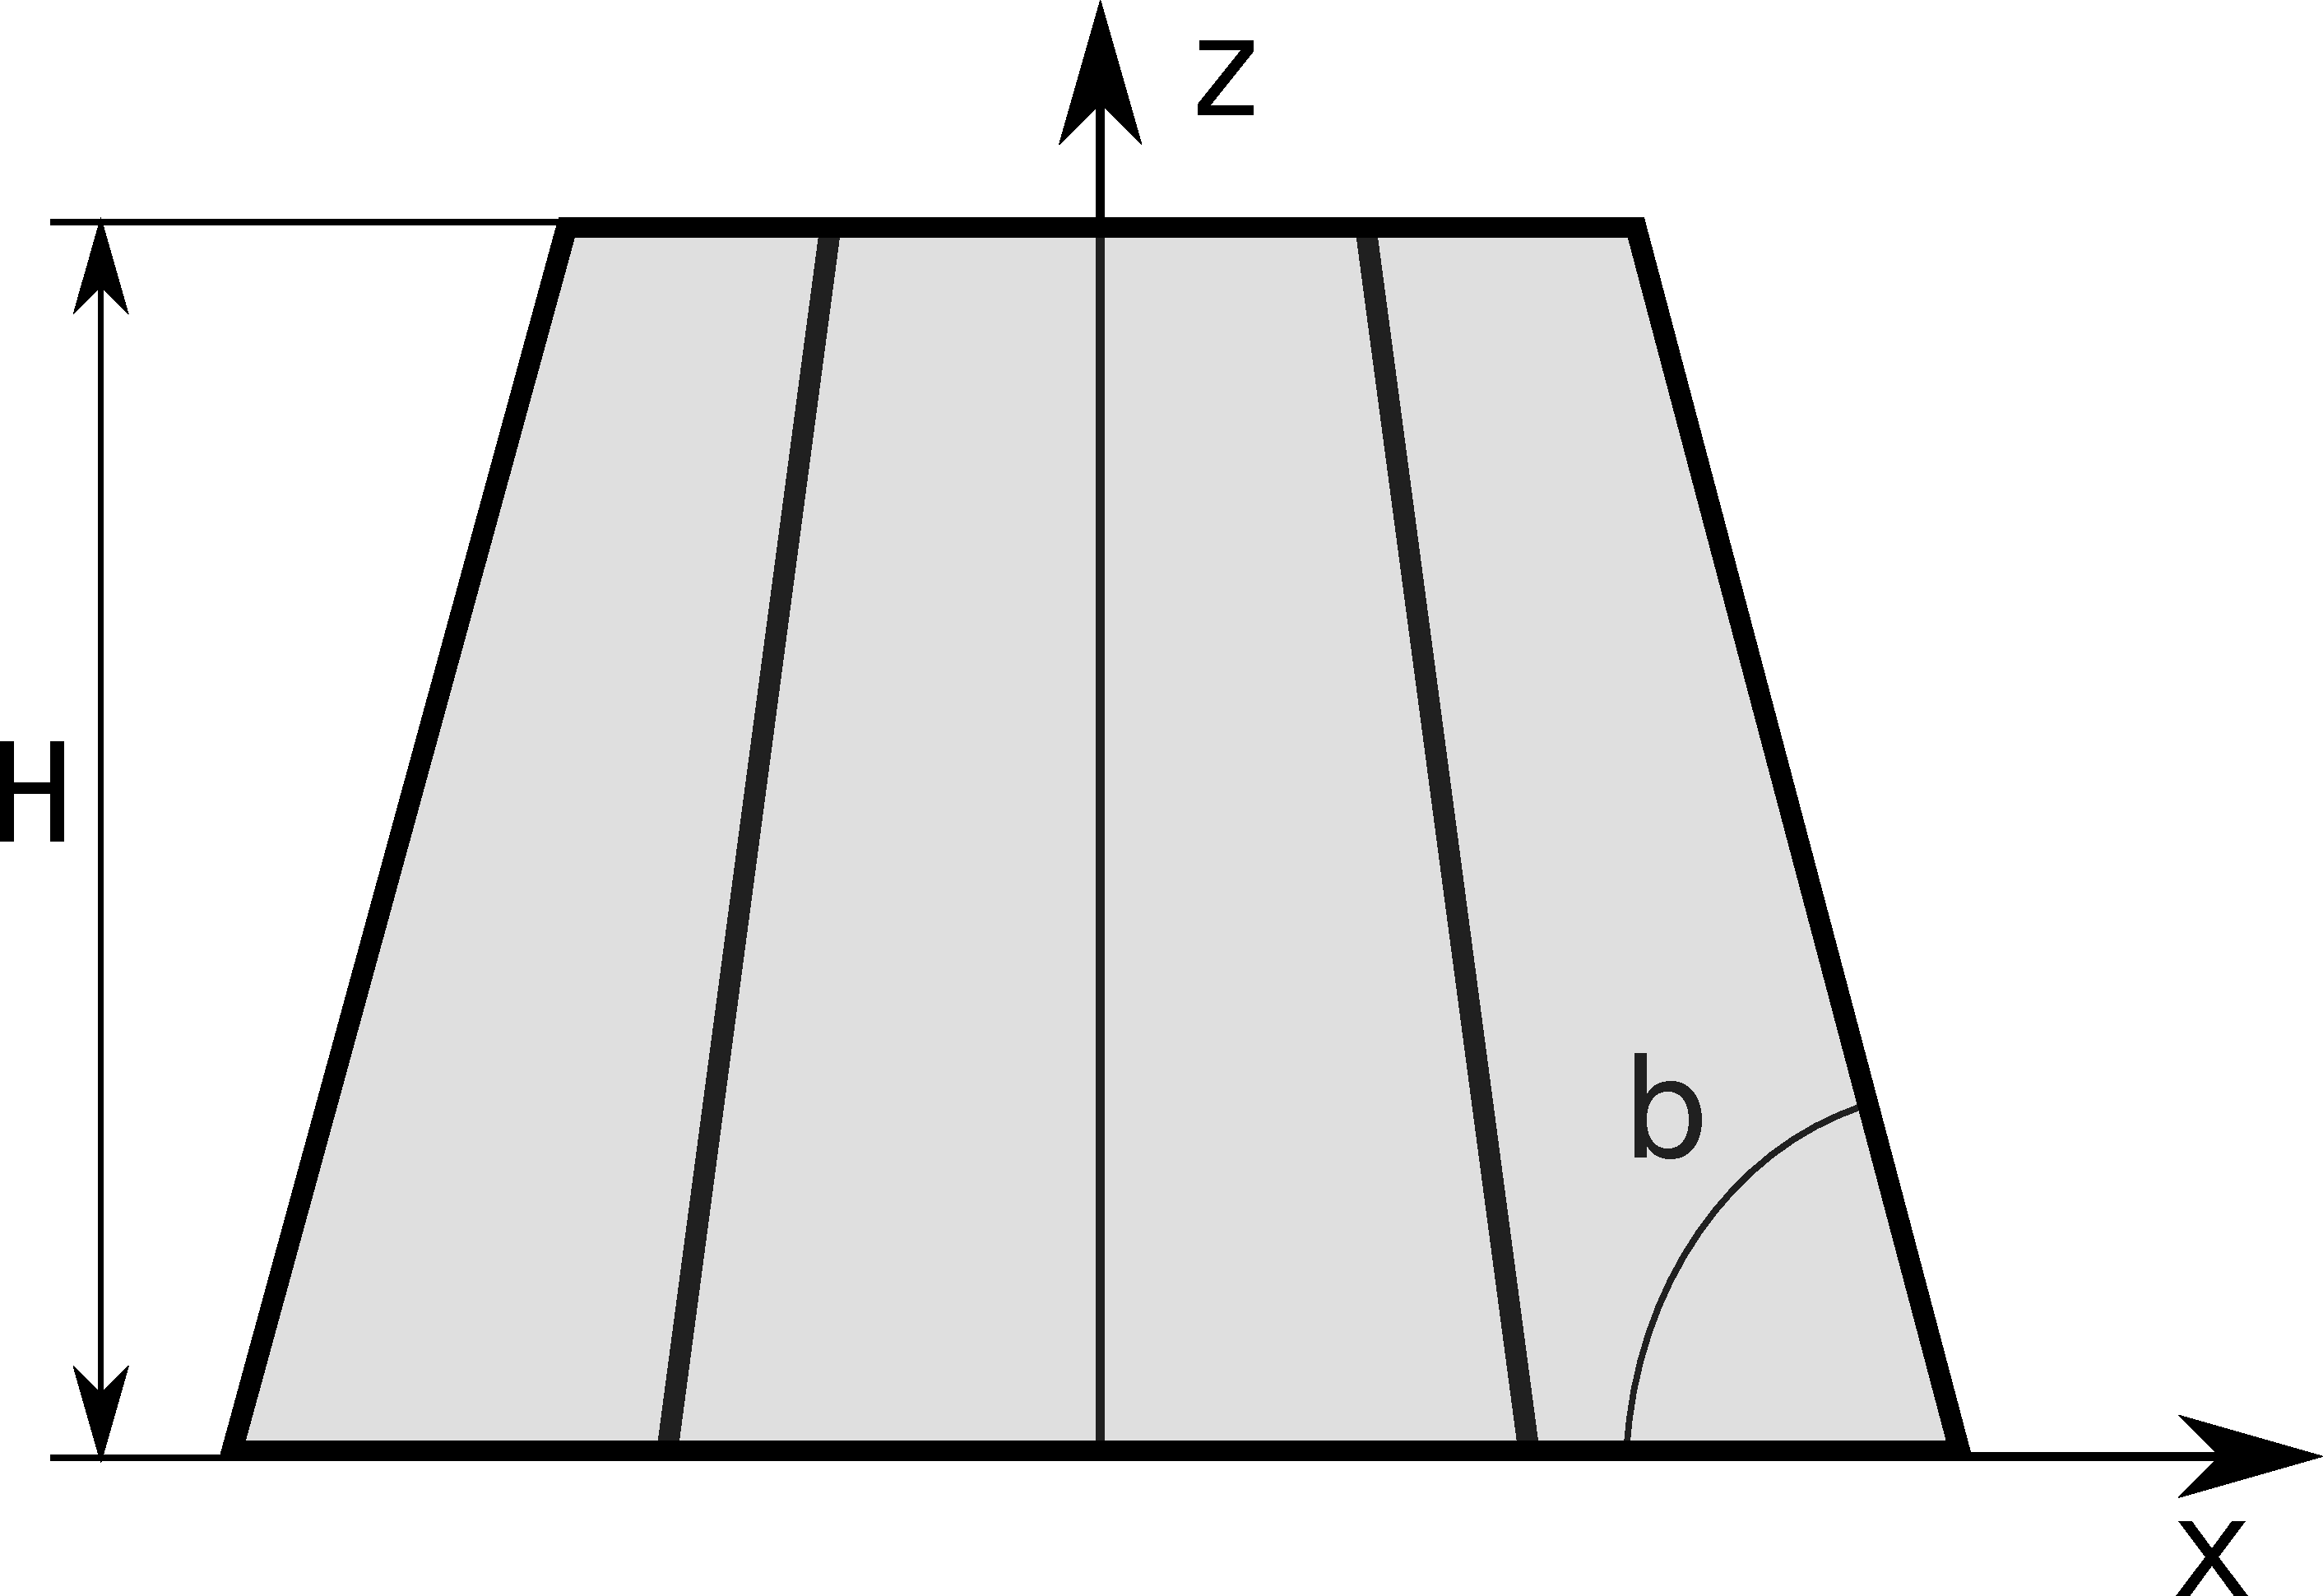
\includegraphics[width=.30\textwidth]{fig/cuts/Cone62dxz.pdf}}}
\hfill
\caption{A truncated pyramid, based on a regular hexagon}
\end{figure}

\FloatBarrier
\paragraph{Syntax and parameters}\strut\\[-2ex plus .2ex minus .2ex]
\begin{lstlisting}
  FormFactorCone6(base_edge,height, alpha)
\end{lstlisting}
with the parameters
\begin{itemize}
\item \texttt{base\_edge}, edge of the regular hexagonal base, $R$,
\item \texttt{height}, $H$,
\item \texttt{alpha}, dihedral angle between the base and a side face, $\alpha$.
\end{itemize}
Note that the orthographic projection does not show~$\alpha$,
but the angle~$\beta$ between the base and a side edge.
They are related through $\sqrt{3}\tan \alpha = 2 \tan \beta$.
The following is written more conveniently in terms of~$\beta$.
The parameters must fulfill
\begin{displaymath}
  H \le (\tan\beta)R.
\end{displaymath}

\paragraph{Form factor, volume, horizontal section}\strut\\
\begin{equation*}
  F \text{~: computed using the generic polyhedron form factor~\cite{ba:ffp},}
\end{equation*}
\begin{equation*}
  V = \tan\beta  \left( R^3- \left(R-\frac{H}{\tan\beta}\right)^3 \right),
\end{equation*}
\begin{equation*}
  S =\dfrac{3\sqrt{3}R^2}{2}.
\end{equation*}

\paragraph{Examples}\strut

\begin{figure}[H]
\begin{center}
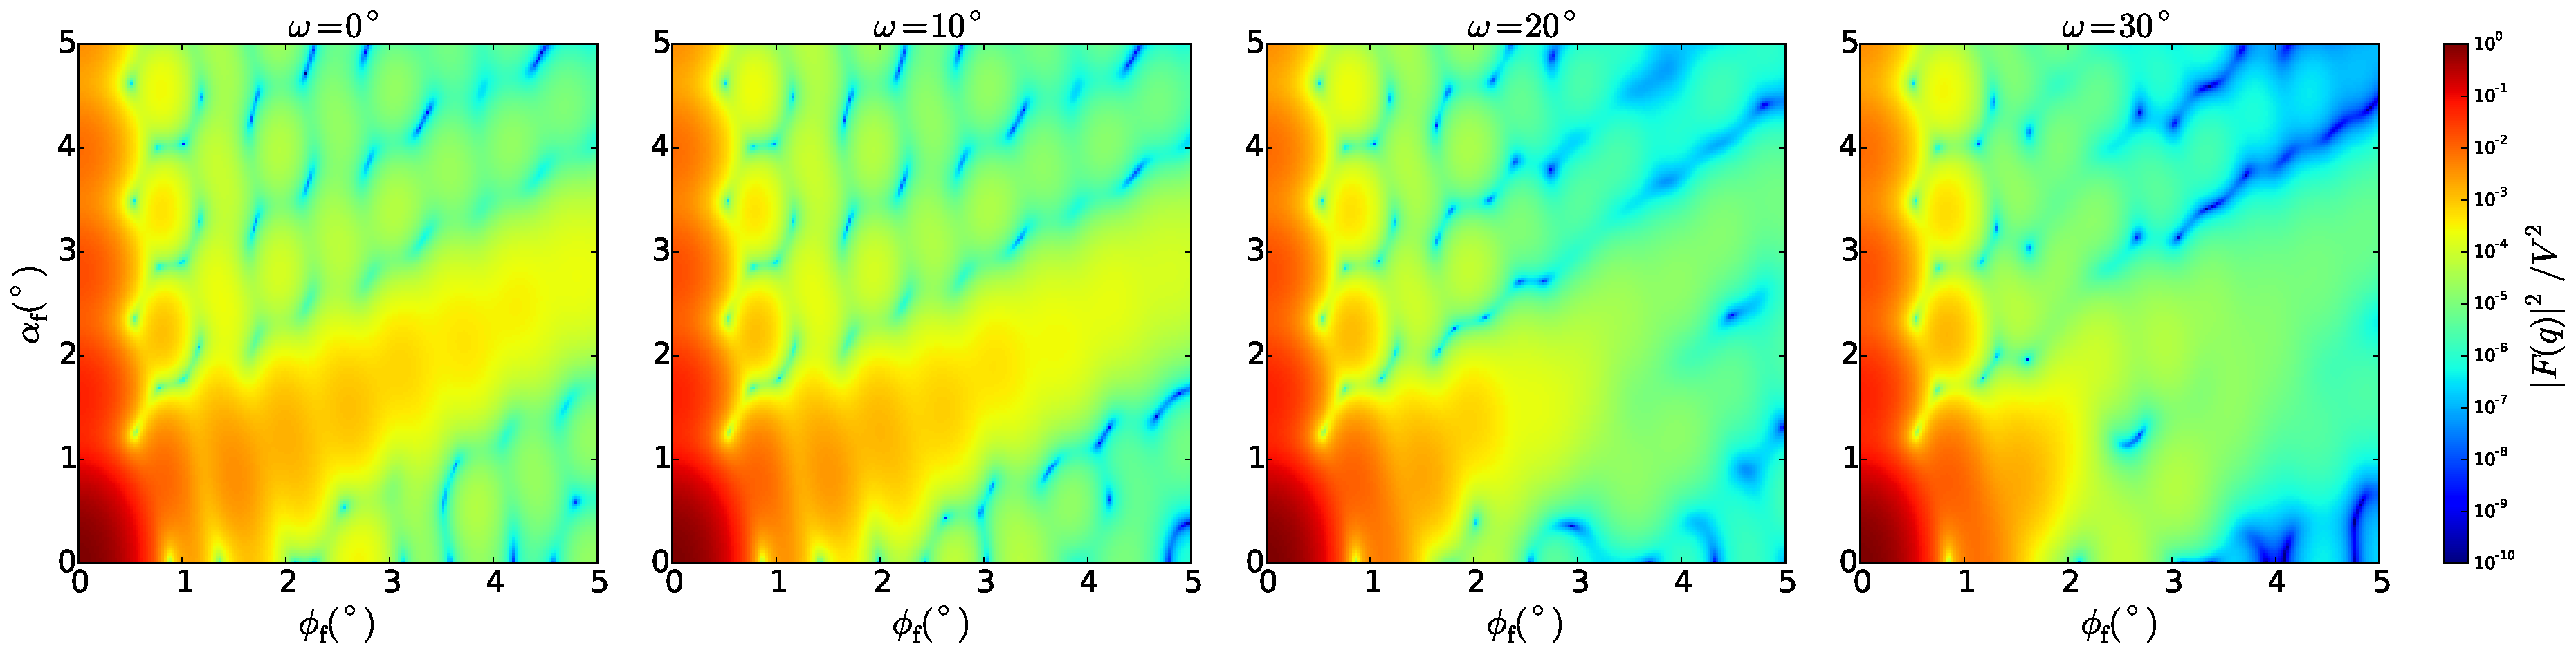
\includegraphics[width=\textwidth]{fig/ff2/ff_Cone6.pdf}
\end{center}
\caption{Normalized intensity $|F|^2/V^2$,
computed with $R=6$~nm, $H=5$~nm, and $\alpha=60^\circ$,
for four different angles~$\omega$ of rotation around the $z$ axis.}
\end{figure}

\paragraph{History}\strut\\
Our parametrization deviates from the form factor \E{Cone6} of \IsGISAXS
\cite[Eq.~2.32]{Laz08} \cite[Eq.~222]{ReLL09}.

Up to \BornAgain-1.5 computed by numeric integration, as in \IsGISAXS.
Since \BornAgain-1.6 higher speed and better accuracy are achieved
by using the generic polyhedron form factor \cite{ba:ffp},
with series expansions near singularities.

%===============================================================================
\ffsection{Cuboctahedron} \label{SCuboctahedron}
%===============================================================================
  \index{Cuboctahedron (form factor)}
  \index{Platonic solids!octahedron}
  \index{FormFactorCuboctahedron@\Code{FormFactorCuboctahedron}}

\paragraph{Real-space geometry}\strut\\

\begin{figure}[H]
\hfill
\subfigure[Perspective]{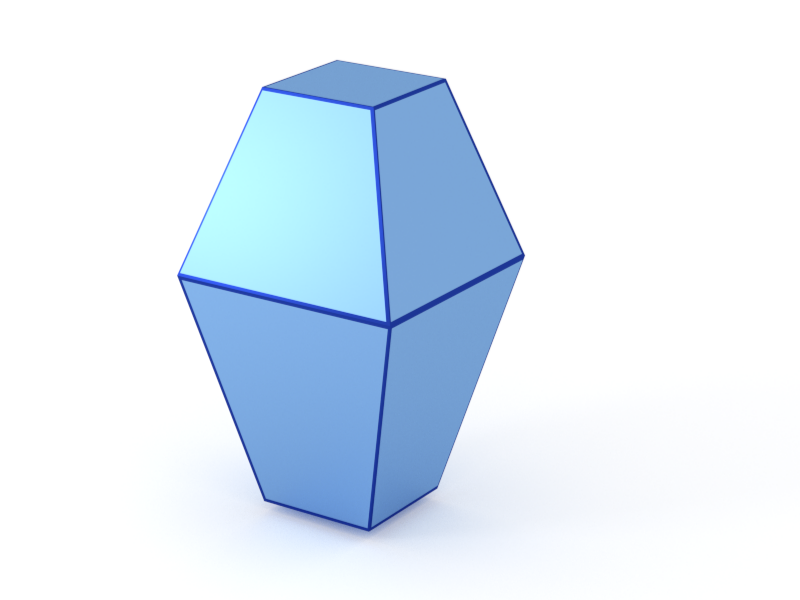
\includegraphics[width=.24\textwidth]{fig/blue/Cuboctahedron3d.png}}
\hfill
\subfigure[Top view]{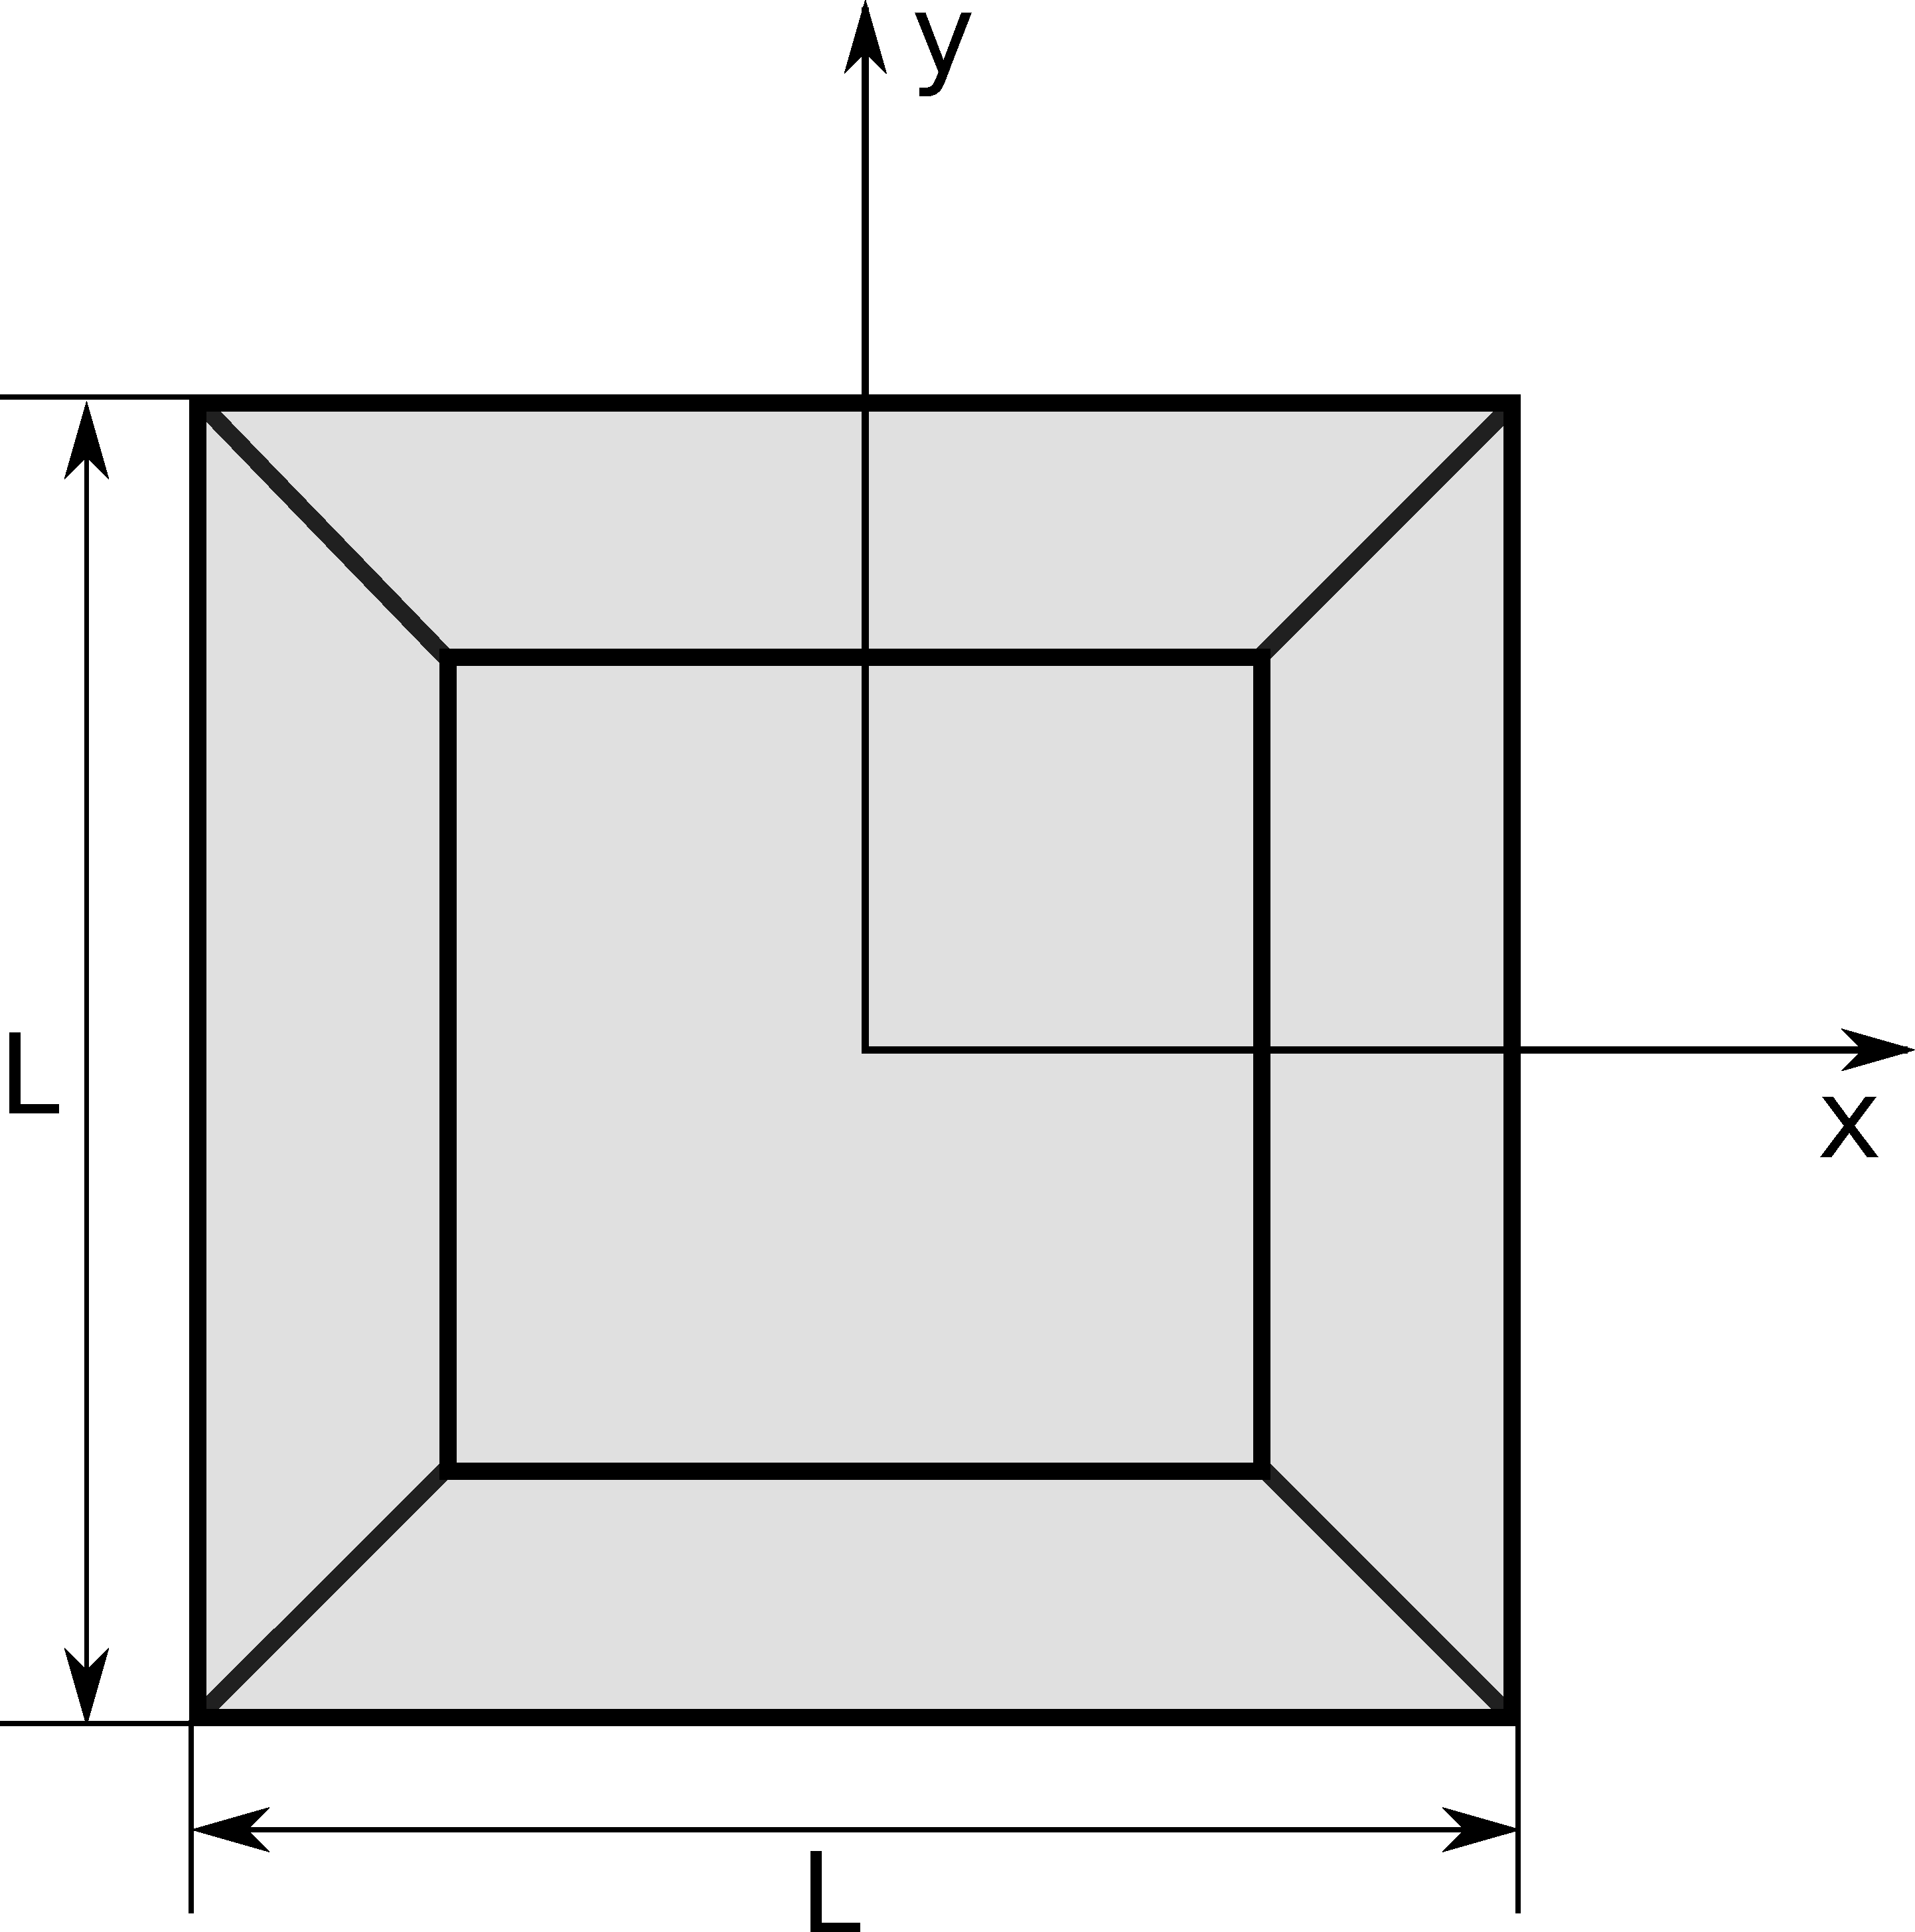
\includegraphics[width=.30\textwidth]{fig/cuts/Cuboctahedron2dxy.pdf}}
\hfill
\subfigure[Side view]{\raisebox{2mm}{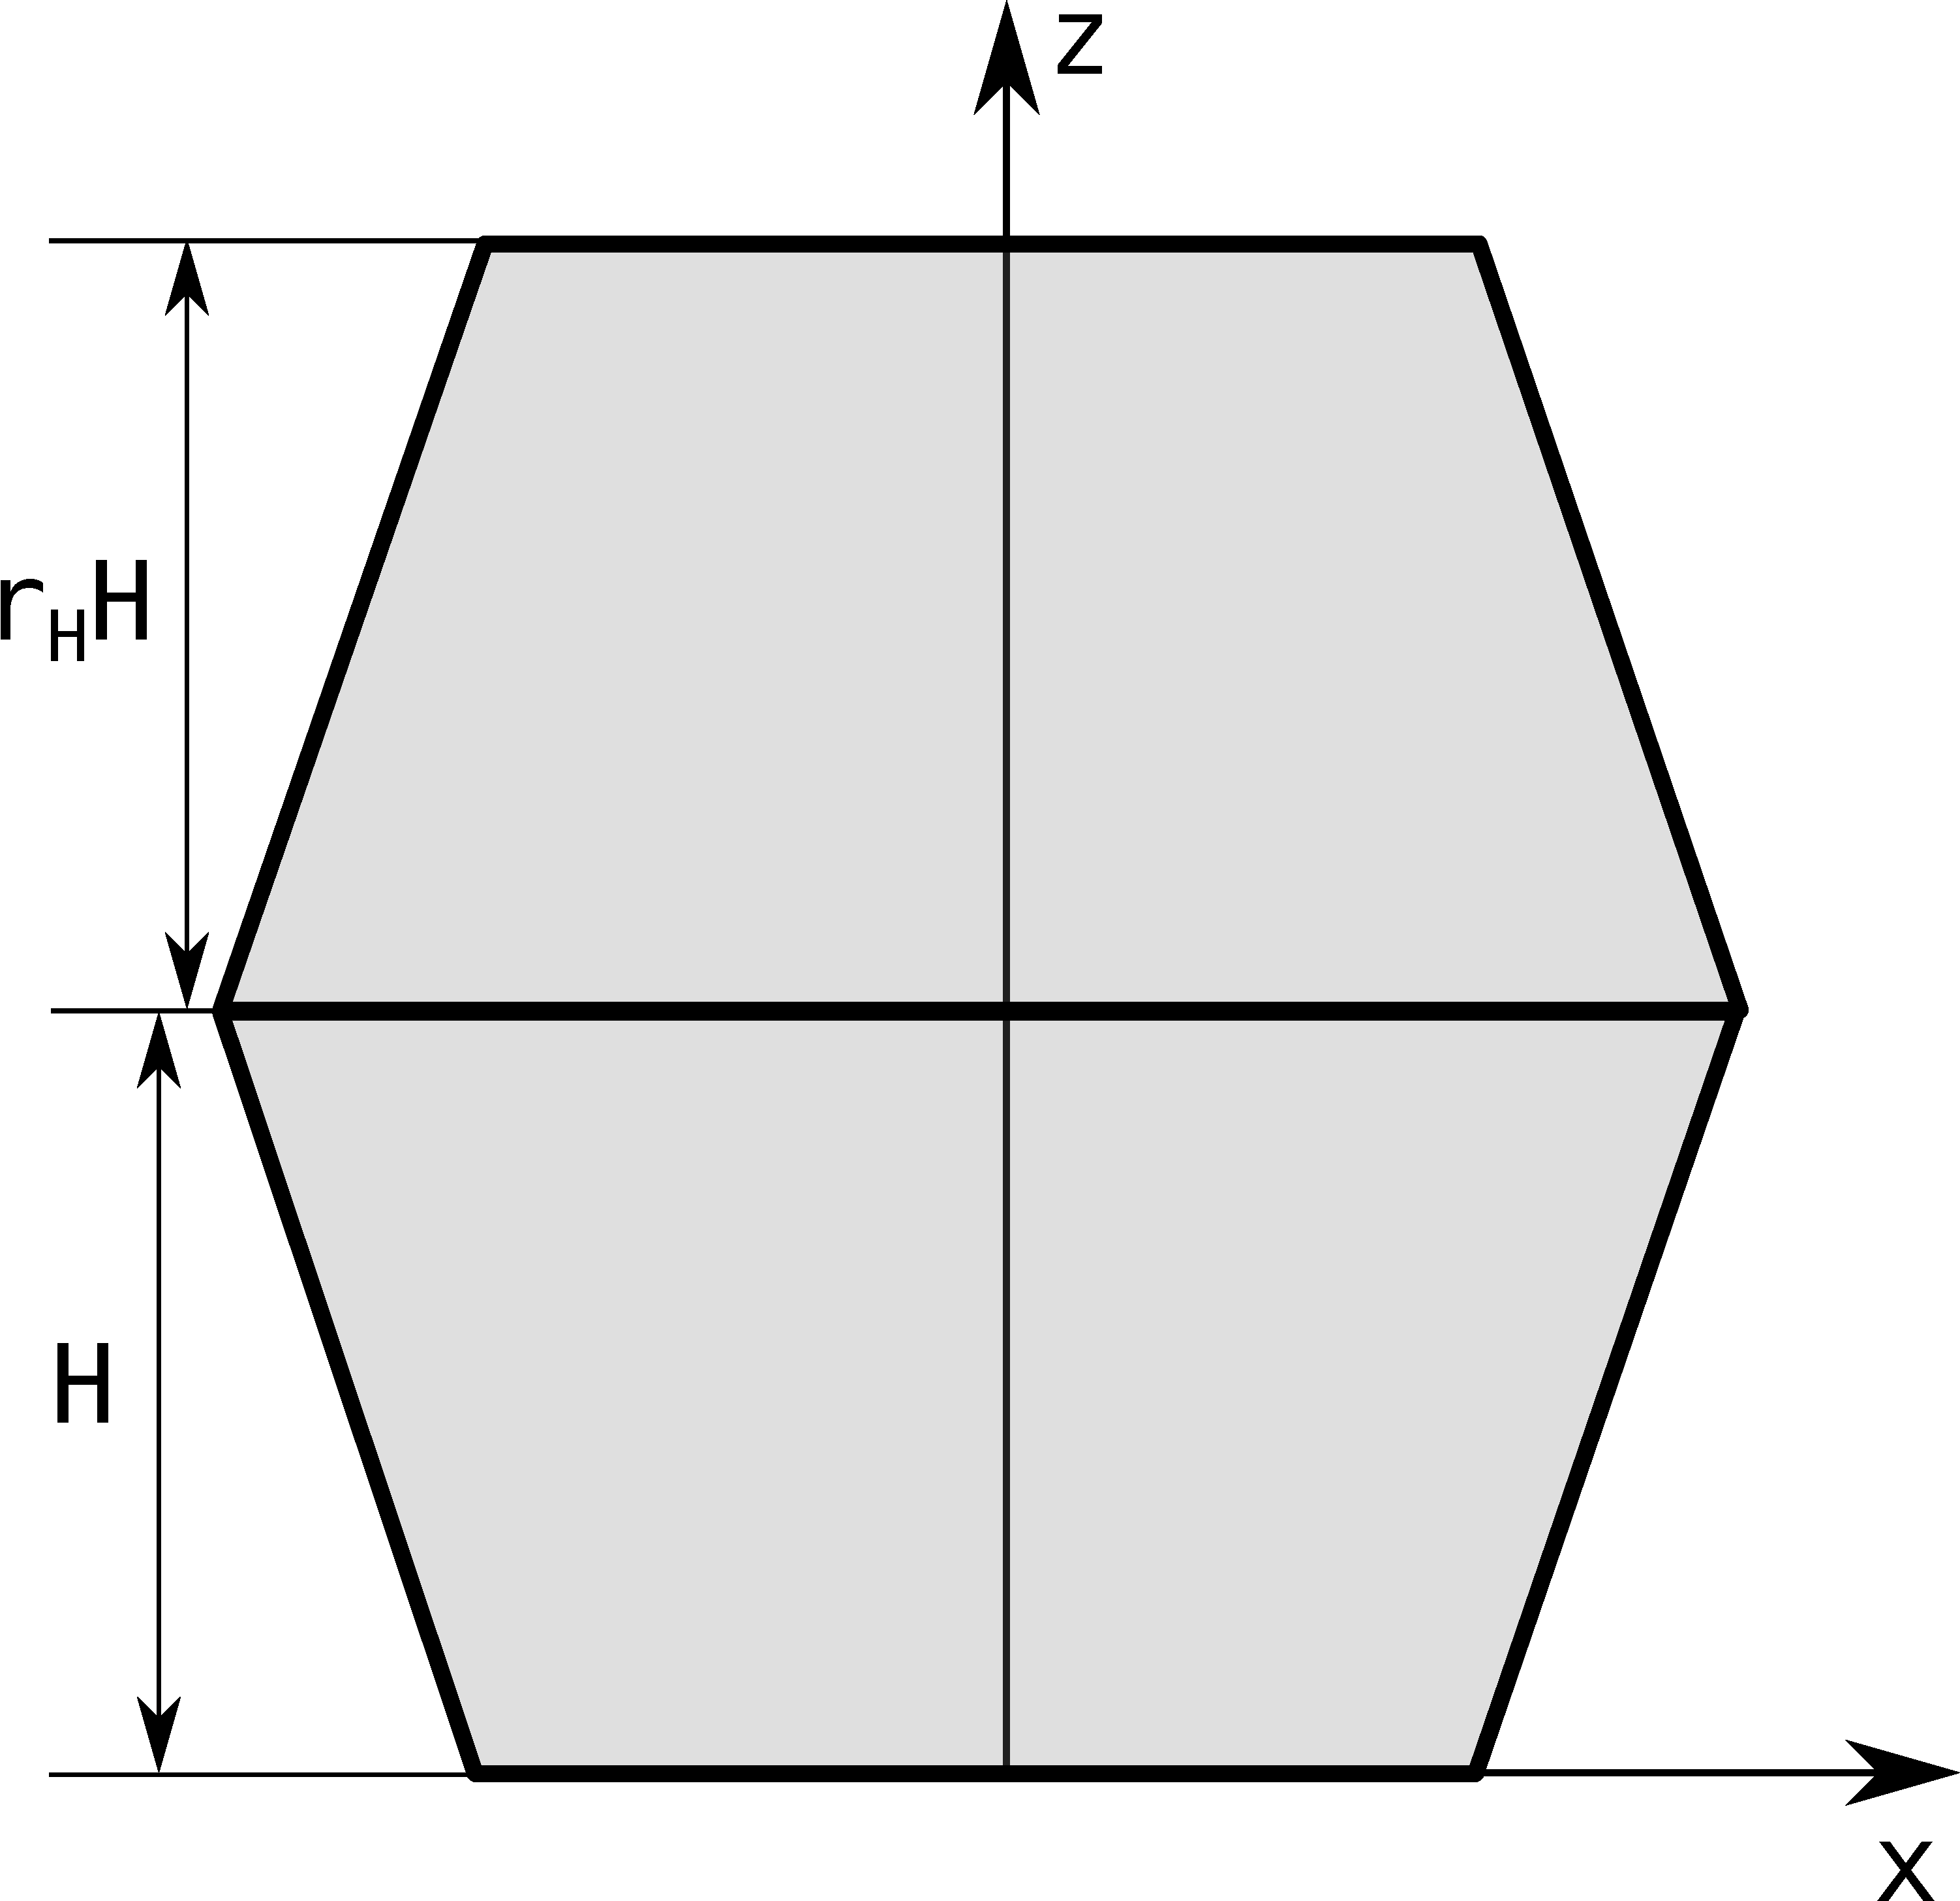
\includegraphics[width=.30\textwidth]{fig/cuts/Cuboctahedron2dxz.pdf}}}
\hfill
\caption{A compound of two truncated pyramids with a common square base
and opposite orientations.}
\end{figure}

\FloatBarrier

\paragraph{Syntax and parameters}\strut\\[-2ex plus .2ex minus .2ex]
\begin{lstlisting}
  FormFactorCuboctahedron(length, height, height_ratio, alpha)
\end{lstlisting}
with the parameters
\begin{itemize}
\item \texttt{length} of the shared square base, $L$,
\item \texttt{height} of the bottom pyramid, $H$,
\item \texttt{height\_ratio} between the top and the bottom pyramid, $r_H$,
\item \texttt{alpha}, angle between the base and a side face, $\alpha$.
\end{itemize}
They must fulfill
\begin{displaymath}
  H \le \frac{\tan\alpha}{2} L
  \quad\text{and}\quad
  r_h H \le \frac{\tan\alpha}{2} L.
\end{displaymath}

\paragraph{Form factor, volume, horizontal section}\strut\\
\begin{equation*}
  F \text{~: computed using the generic polyhedron form factor~\cite{ba:ffp},}
\end{equation*}
\begin{equation*}
  V= \dfrac{1}{6} \tan(\alpha)L^3 \Big[ 2
         - \Big(1 - \dfrac{2H }{L\tan(\alpha)} \Big)^3
           - \Big(1 - \dfrac{2 r_H
             H}{L\tan(\alpha) }\Big)^3\Big],
\end{equation*}
\begin{equation*}
  S =L^2.
\end{equation*}

\paragraph{Examples}\strut

\begin{figure}[H]
\begin{center}
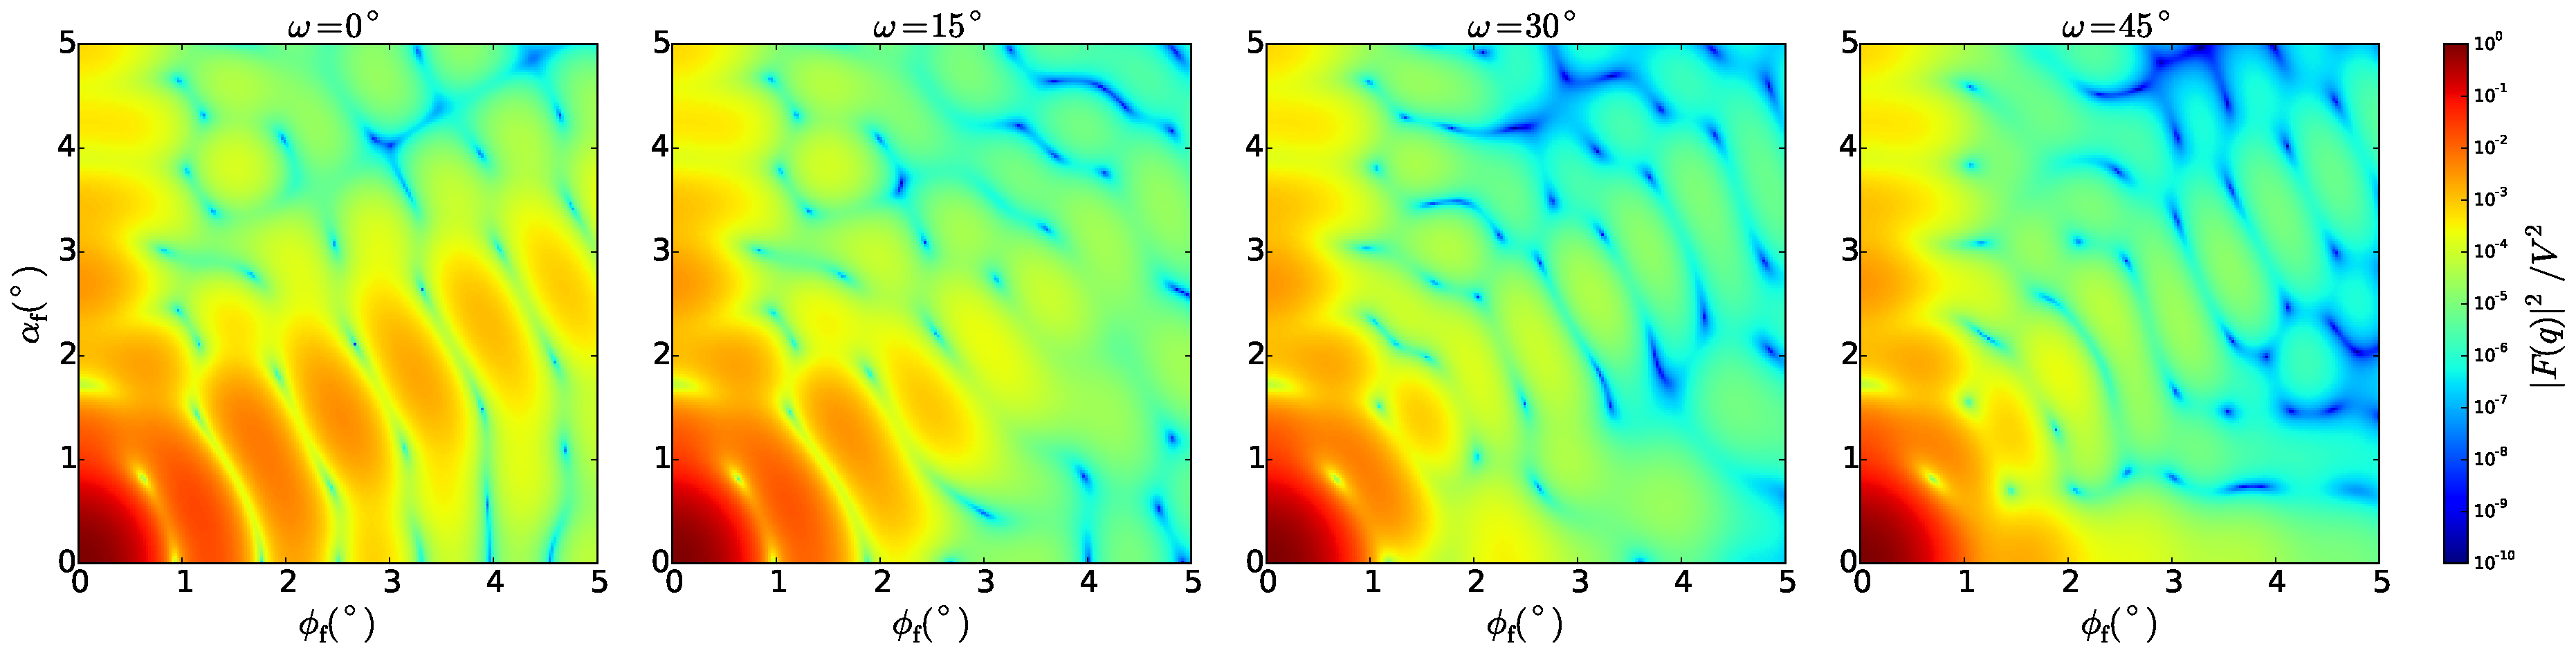
\includegraphics[width=\textwidth]{fig/ff2/ff_Cuboctahedron.pdf}
\end{center}
\caption{Normalized intensity $|F|^2/V^2$,
computed with $L=8$~nm, $H=5$~nm, $r_H=0.5$, and $\alpha=60^\circ$,
for four different angles~$\omega$ of rotation around the $z$ axis.}
\end{figure}

\paragraph{History}\strut\\
Agrees with \E{Cuboctahedron} form factor of \IsGISAXS\
\cite[Eq.~2.34]{Laz08} \cite[Eq.~218]{ReLL09},
except for different parametrization $L=2R_{\rm{\Code{IsGISAXS}}}$.
Since \BornAgain-1.6 implemented
using the generic polyhedron form factor \cite{ba:ffp}.


%===============================================================================
\ffsection{Cylinder} \label{SCylinder}
%===============================================================================
  \index{Cylinder (form factor)}
  \index{FormFactorCylinder@\Code{FormFactorCylinder}}

\paragraph{Real-space geometry}\strut\\

\begin{figure}[H]
\hfill
\subfigure[Perspective]{
\includegraphics[width=.24\textwidth]{fig/blue/Cylinder3d.png}}
\hfill
\subfigure[Top view]{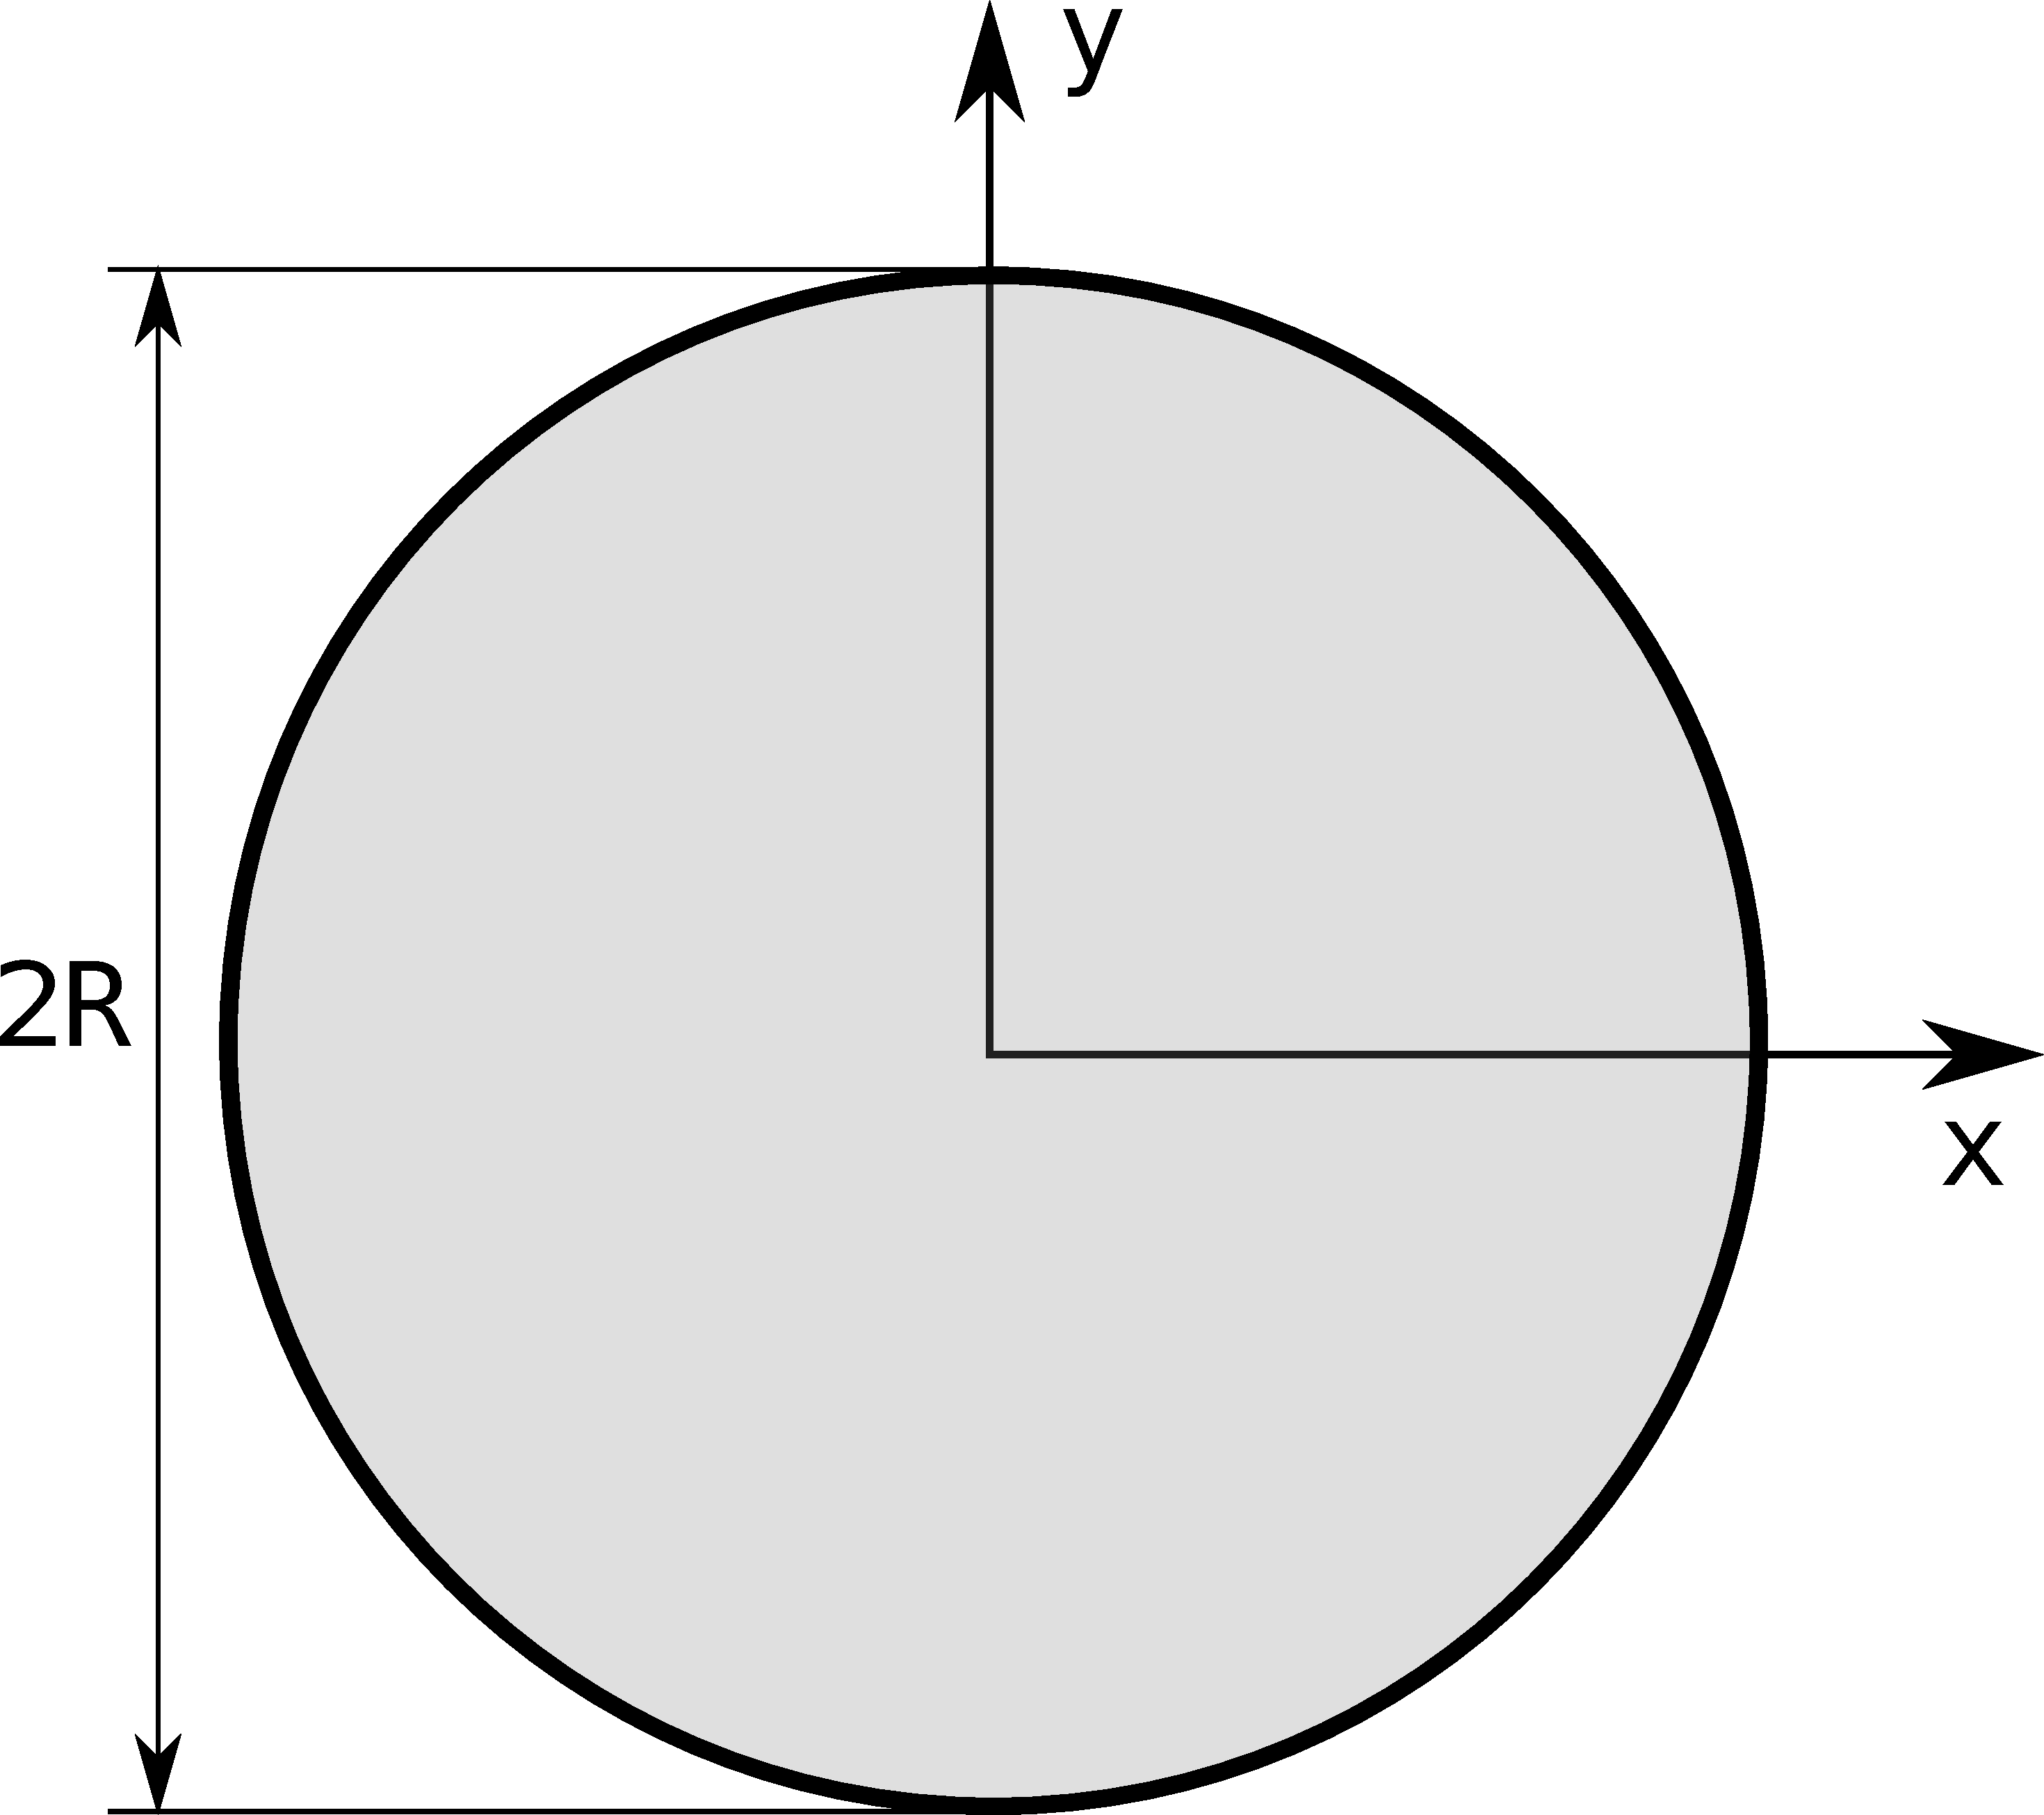
\includegraphics[width=.30\textwidth]{fig/cuts/Cylinder2dxy.pdf}}
\hfill
\subfigure[Side view]{\raisebox{-2.5mm}{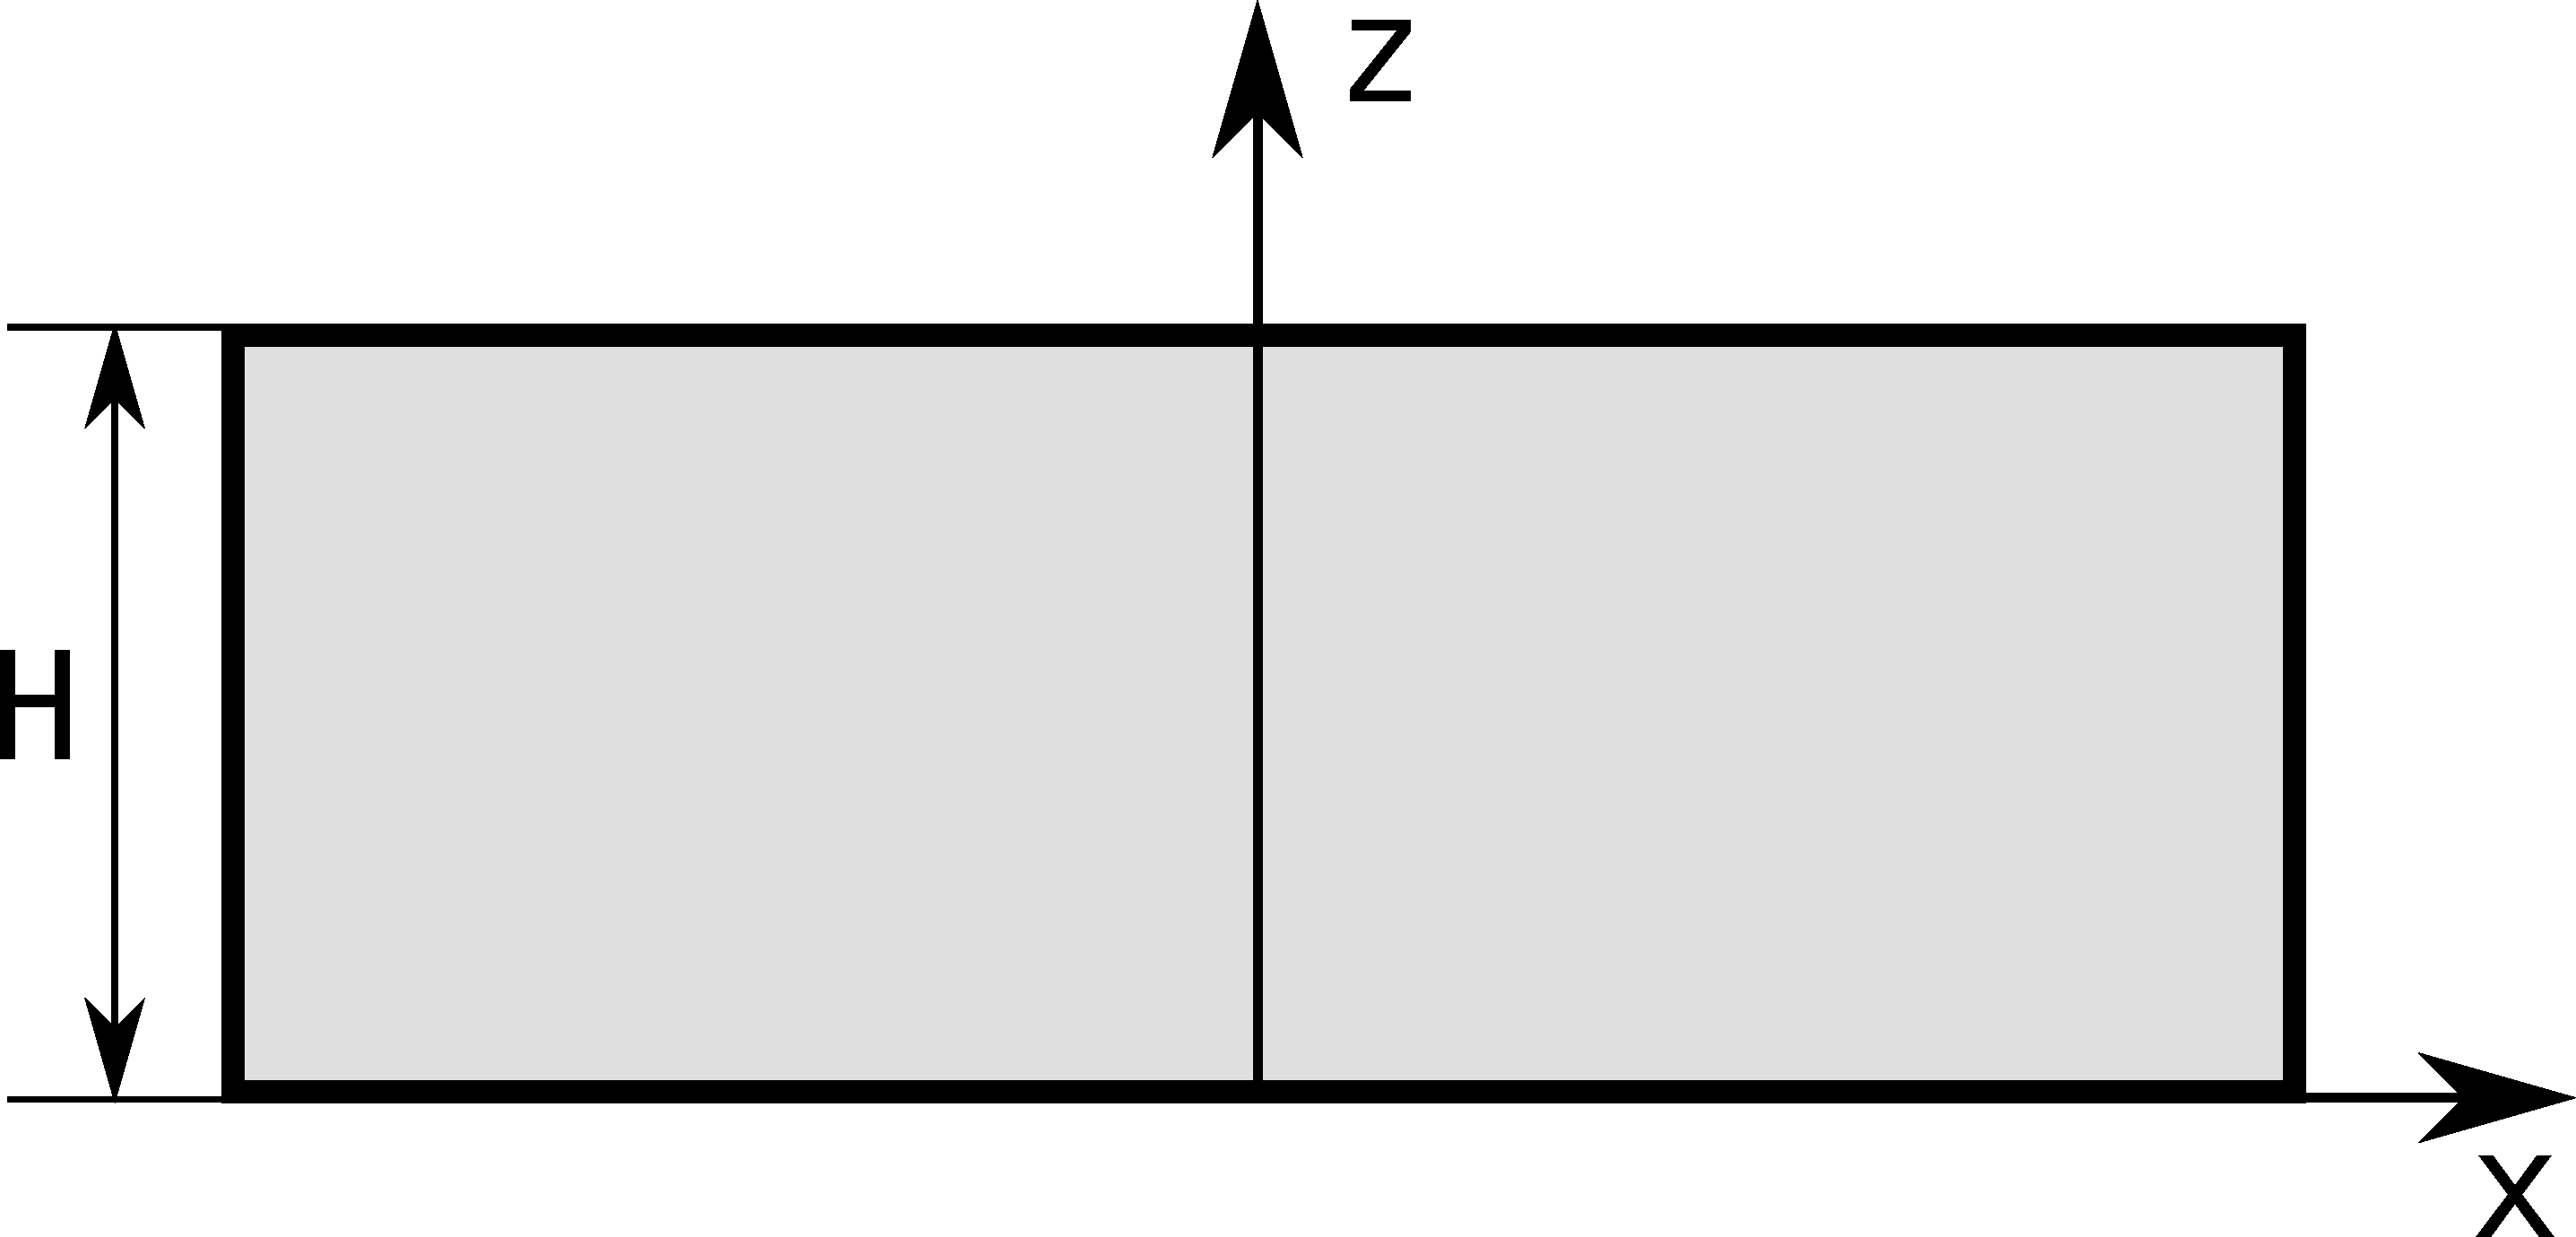
\includegraphics[width=.30\textwidth]{fig/cuts/Cylinder2dxz.pdf}}}
\hfill
\caption{An upright circular cylinder.}
\end{figure}

\paragraph{Syntax and parameters}\strut\\[-2ex plus .2ex minus .2ex]
\begin{lstlisting}
  FormFactorCylinder(radius, height)
\end{lstlisting}
with the parameters
\begin{itemize}
\item \texttt{radius} of the circular base, $R$,
\item \texttt{height}, $H$.
\end{itemize}

\paragraph{Form factor, volume, horizontal section}\strut\\
Notation:
\begin{equation*}
  q_{\parallel} \coloneqq \sqrt{q_x^2+q_y^2}.
\end{equation*}
Note that this does \E{not} involve the sesquilinear product
$|q_x|^2=q_x^* q_x$ but the plain product $q_xq_x$ of complex numbers
(and analogous for~$q_y$).

Results:
\begin{equation*}
  F=  2\pi R^2 H  \sinc\left(q_ z \frac{H}{2}\right) \exp\left(i q_ z \frac{H}{2}\right)
    \frac{J_1(q_{\parallel} R )}{q_{\parallel} R },
\end{equation*}
\begin{equation*}
  V = \pi R^2 H,
\end{equation*}
\begin{equation*}
  S=\pi R^2.
\end{equation*}

\paragraph{Examples}\strut

\begin{figure}[H]
\begin{center}
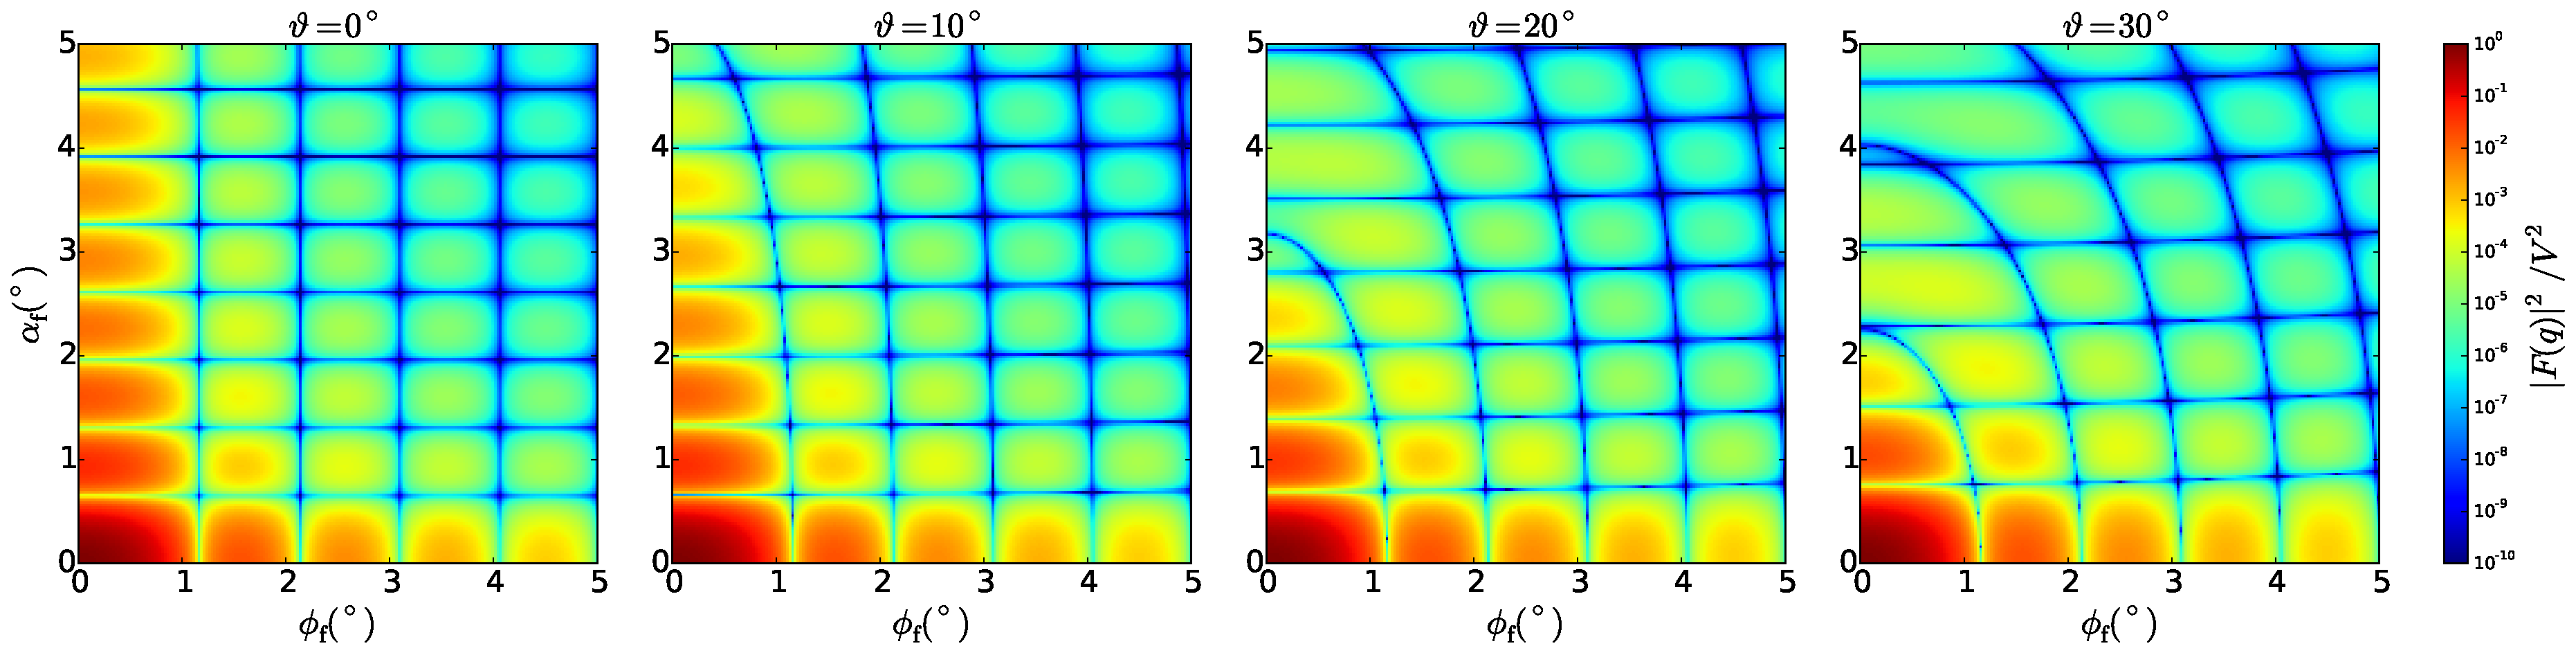
\includegraphics[width=\textwidth]{fig/ff2/ff_Cylinder.pdf}
\end{center}
\caption{Normalized intensity $|F|^2/V^2$,
computed with $R=3$~nm and $H=8.8$~nm,
for four different tilt angles~$\vartheta$ (rotation around the $y$ axis).}
\end{figure}

\paragraph{History and Derivation}\strut\\
For real wave vectors, this form factor is well known;
it goes back to Lord Rayleigh.
In \IsGISAXS, it has been implemented as form factor \E{Cylinder}
\cite[Eq.~2.27]{Laz08} \cite[Eq.~223]{ReLL09},
allowing for complex wavevectors.

Since it is not obvious that the standard formula also holds for complex~$\q$,
let us provide a derivation. We only consider the integral over the polar angle,
\begin{equation}
  I(\q) \coloneqq \int_0^{2\pi}\!\d\varphi\,\exp\left(iq_xr\sin\varphi+iq_yr\cos\varphi\right).
\end{equation}
With the abbreviations $a\coloneqq r(q_x+iq_y)/2$ and $b\coloneqq r(q_x-iq_y)/2$,
\begin{equation}
  I(\q) = \int_0^{2\pi}\!\d\varphi\,\exp\left(a\e^{i\varphi}-b\e^{-i\varphi}\right).
\end{equation}
Expansion of the exponential, combined with a binomial expansion of its argument, yields
\begin{equation}
  I(\q)
  = \int_0^{2\pi}\!\d\varphi\,
  \sum_{n=0}^\infty\sum_{k=0}^n(-)^k\frac{a^{n-k}b^{k}}{(n-k)!k!}\e^{i(n-2k)\varphi}.
\end{equation}
The integral over $\varphi$ vanishes except for $n=2k$. Hence
\begin{equation}
  I(\q)
  = 2\pi \sum_{k=0}^\infty(-)^k\frac{{\sqrt{ab}\,}^{2k}}{k!k!}
  = 2\pi J_0\left(rq_\parallel\right).
\end{equation}
Integration over~$r$ then yields the in-plane contribution to the form factor~$F(\q)$.


%===============================================================================
\ffsection{Dodecahedron} \label{SDodecahedron}
%===============================================================================
  \index{Dodecahedron (form factor)}
  \index{Platonic solids!dodecahedron}
  \index{FormFactorDodecahedron@\Code{FormFactorDodecahedron}}

\paragraph{Real-space geometry}\strut\\

\begin{figure}[H]
\strut\hfill
%\subfigure[Perspective]
{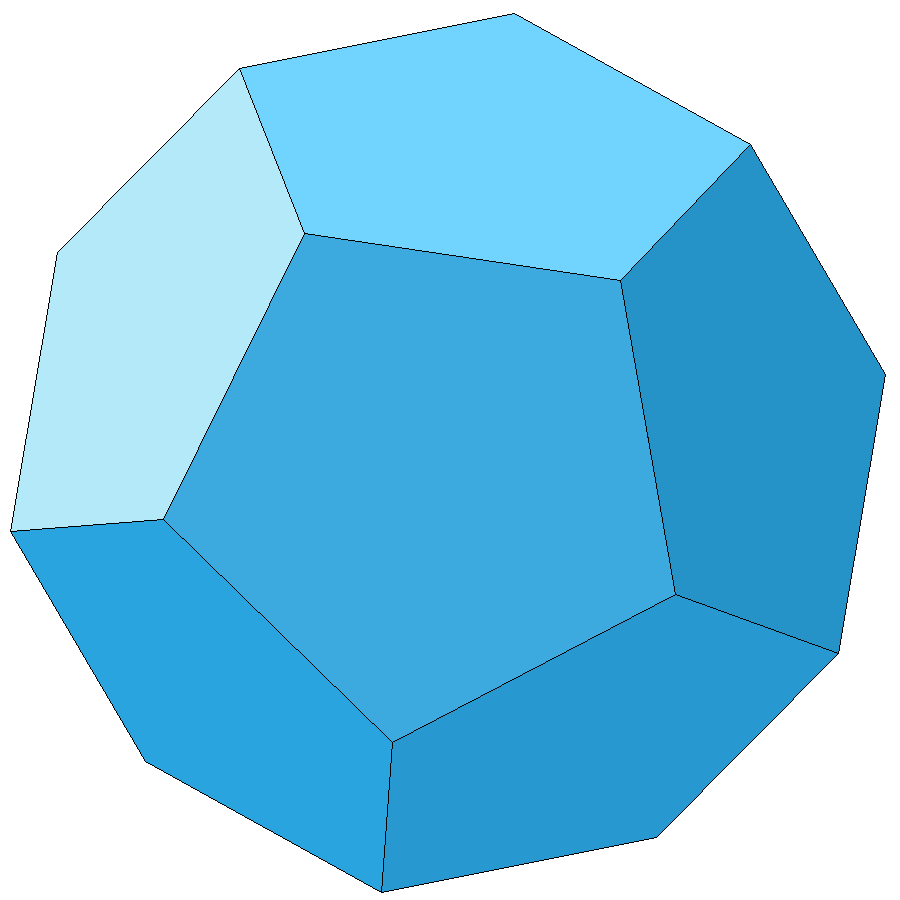
\includegraphics[width=.24\textwidth]{fig/blue/Dodecahedron3d.png}}
%\hfill
%\subfigure[Top view]{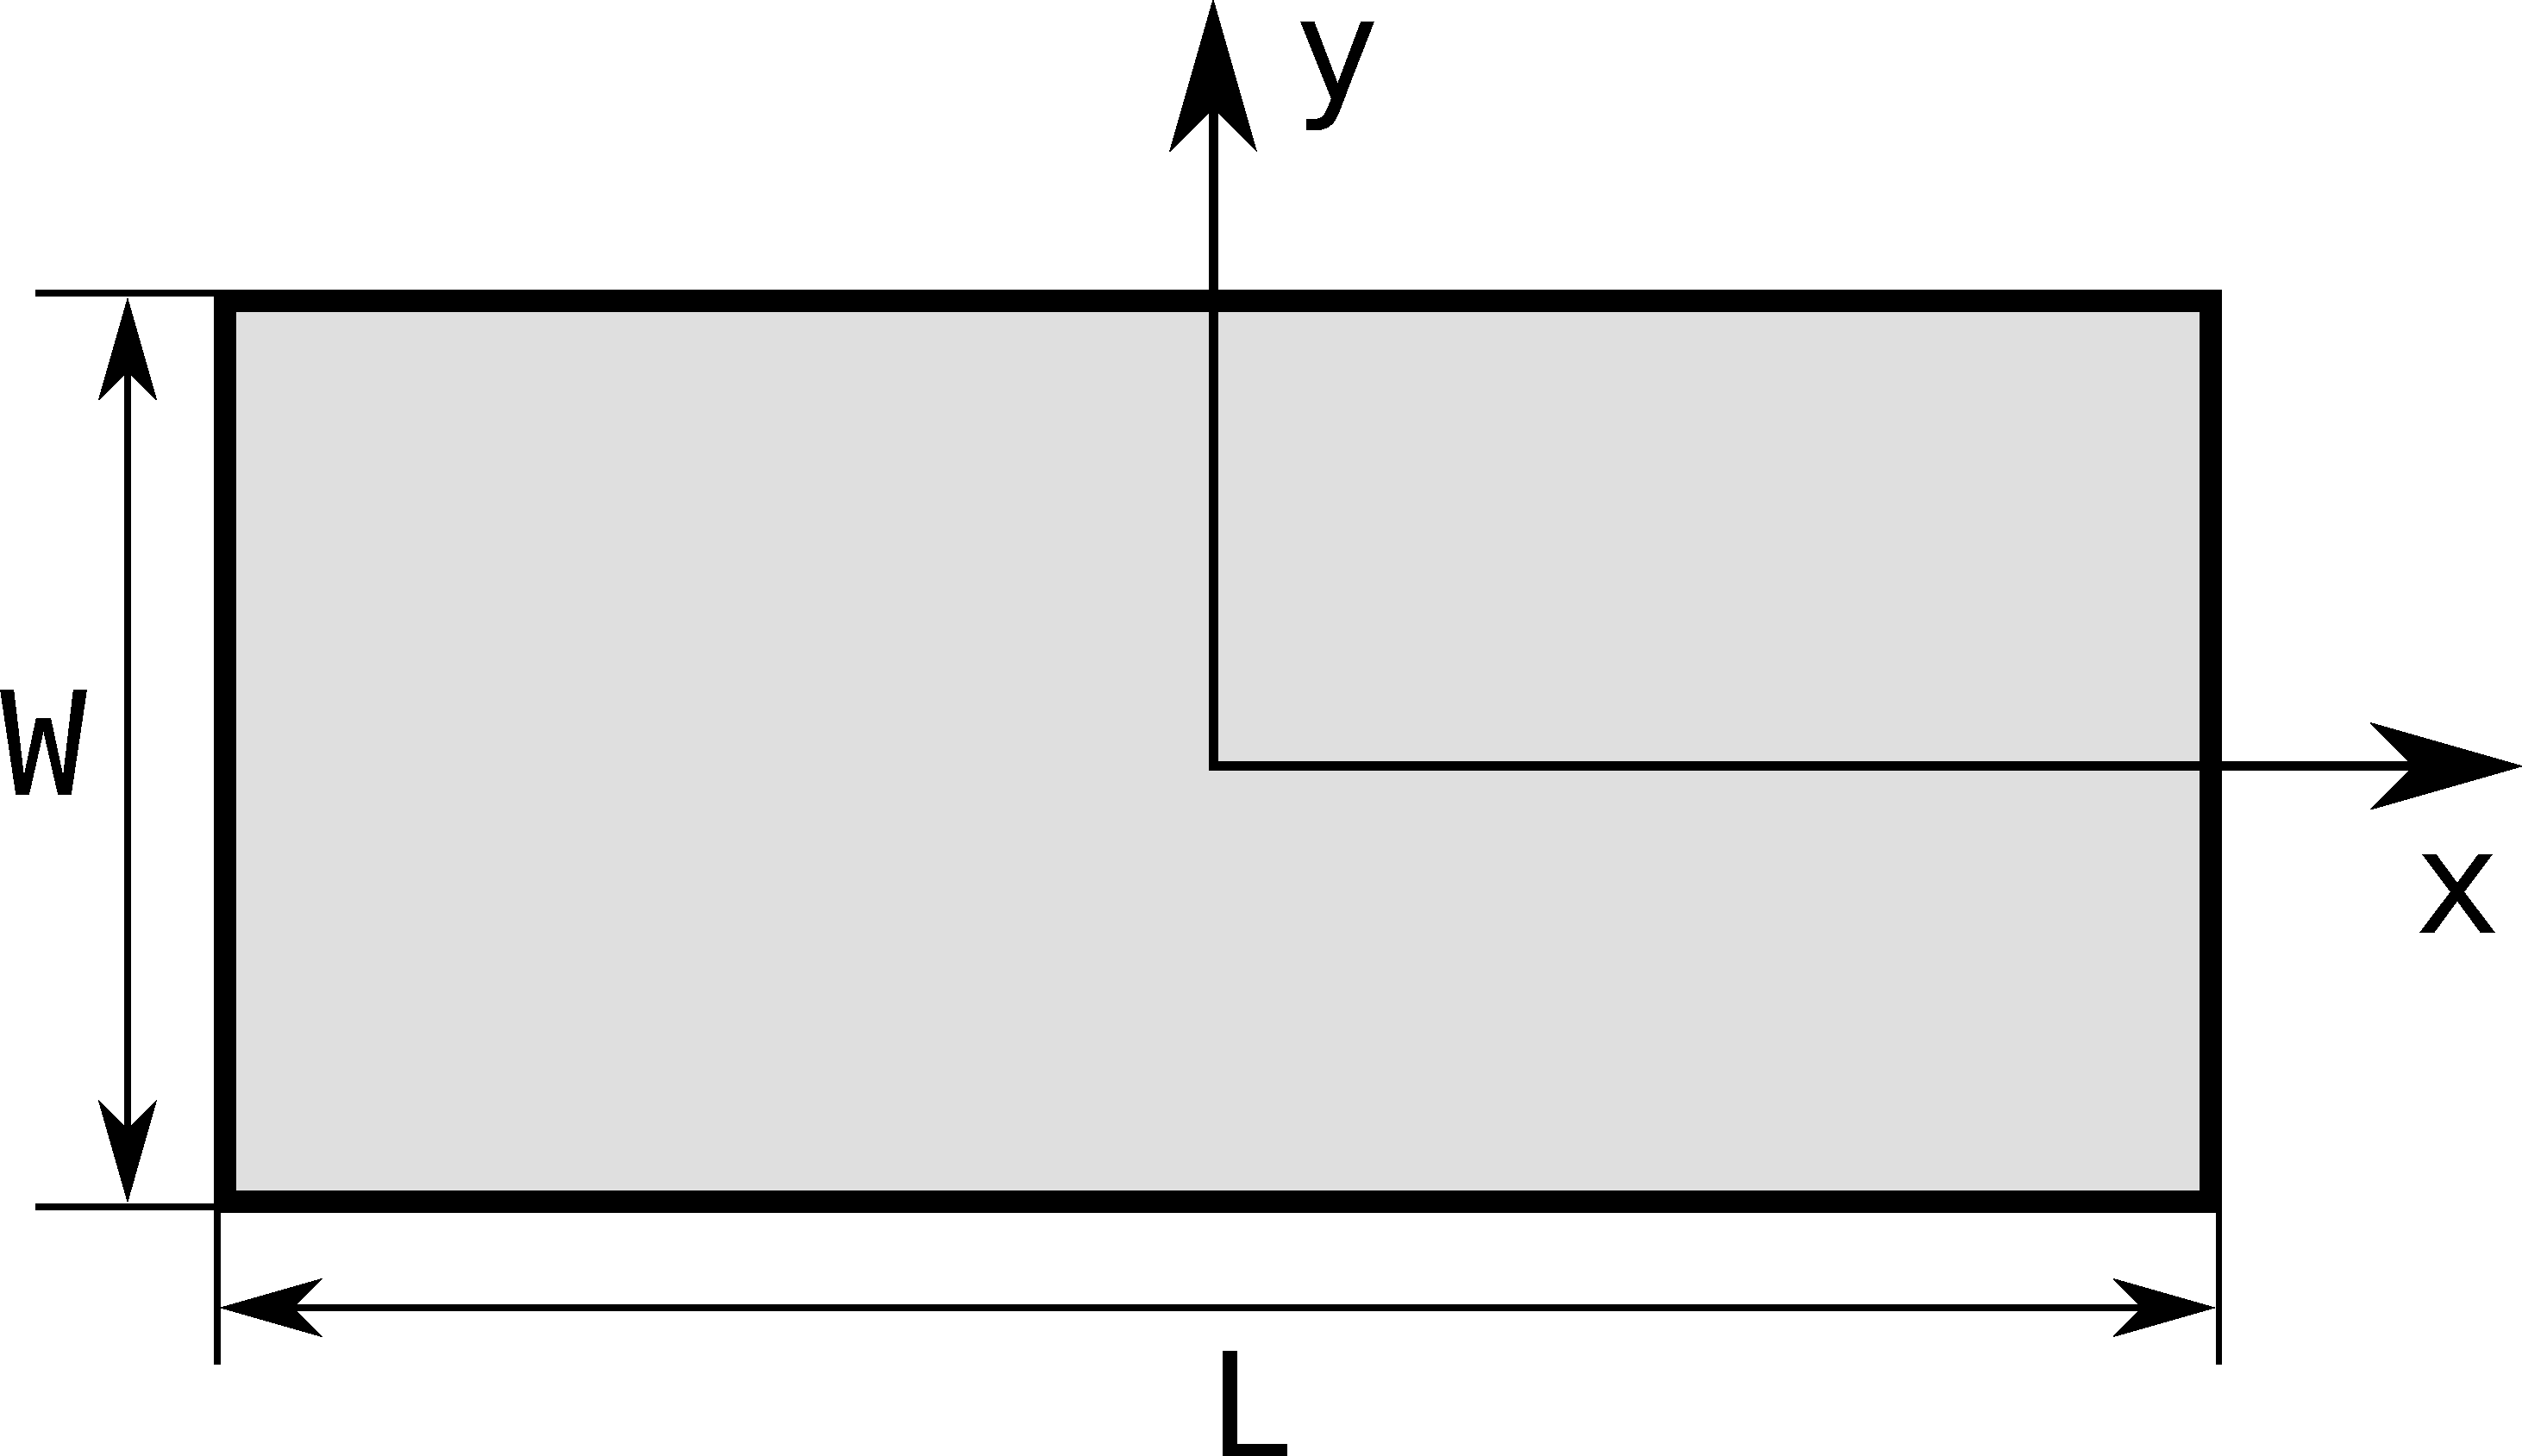
\includegraphics[width=.30\textwidth]{fig/cuts/Box2dxy.pdf}}
%\hfill
%\subfigure[Side view]{\raisebox{2mm}{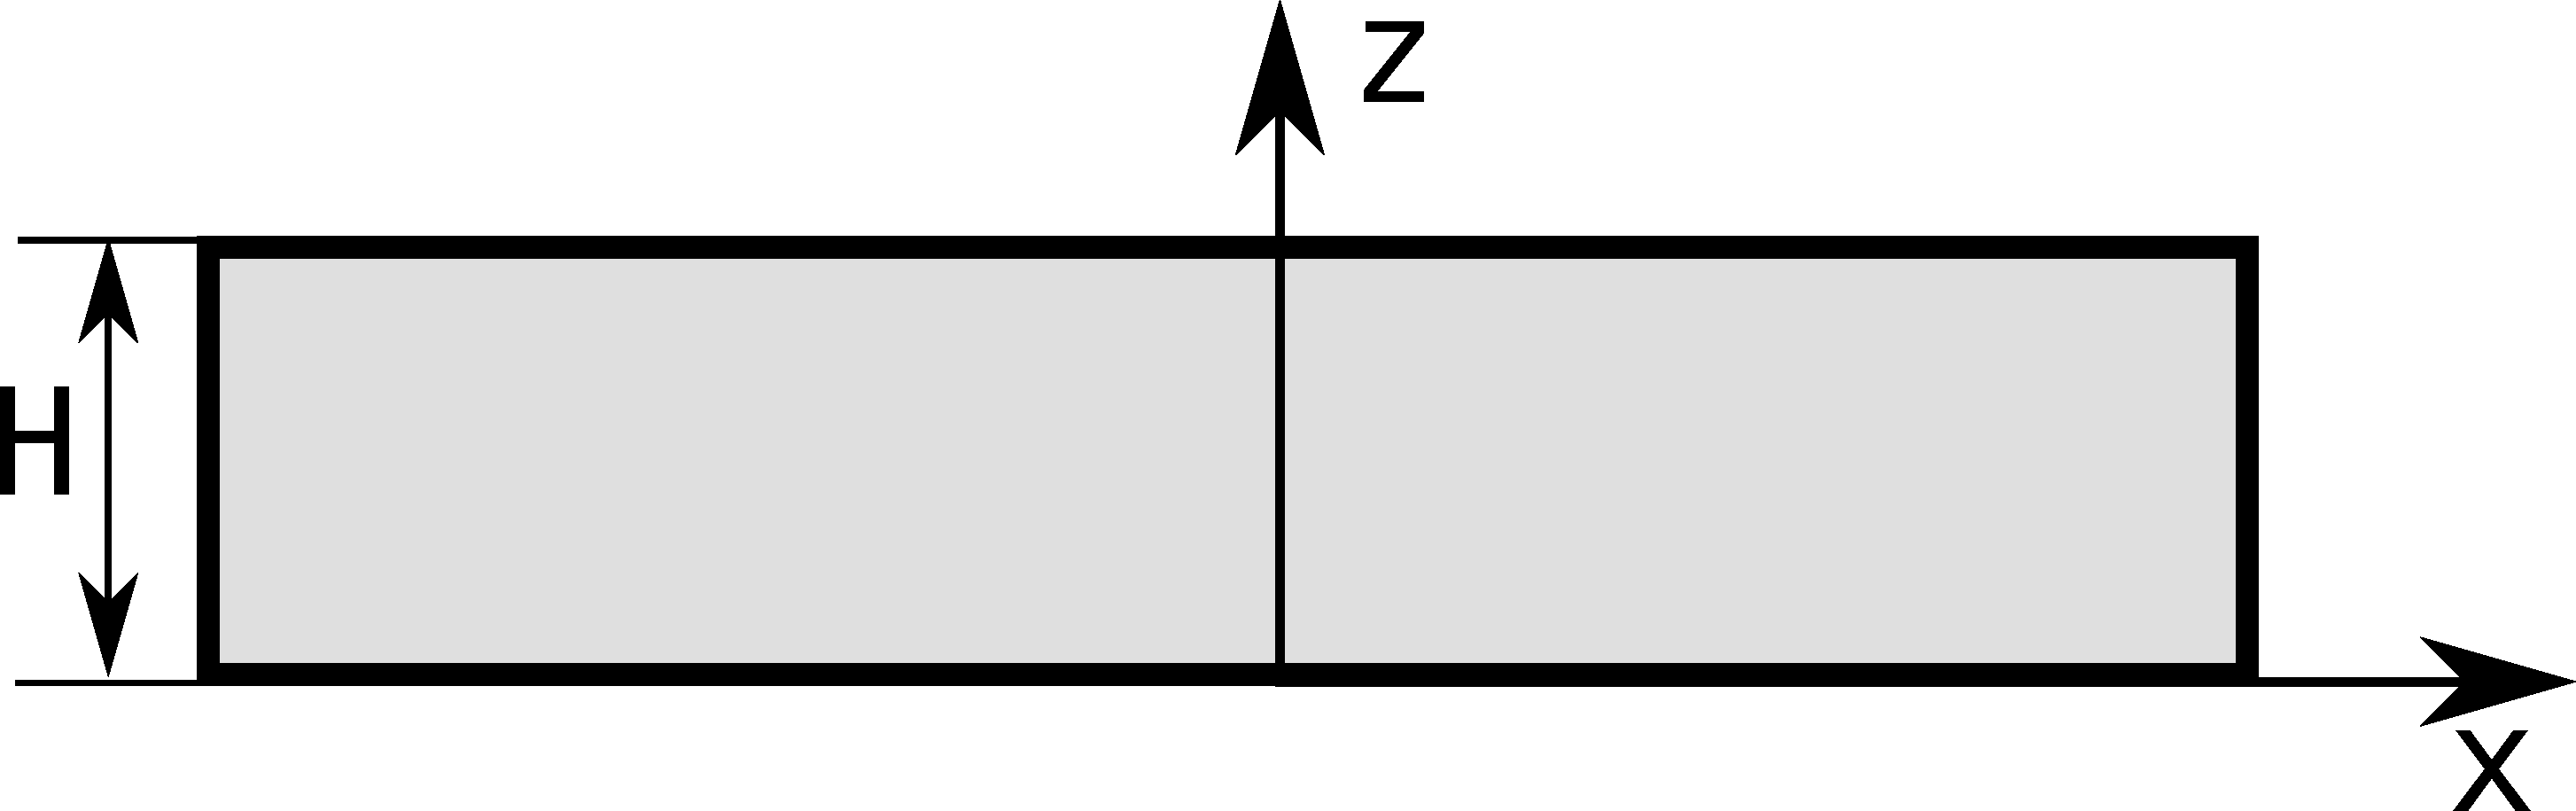
\includegraphics[width=.30\textwidth]{fig/cuts/Box2dxz.pdf}}}
\hfill\strut
\caption{A regular dodecahedron.}
\end{figure}

\FloatBarrier

\paragraph{Syntax and parameters}\strut\\[-2ex plus .2ex minus .2ex]
\begin{lstlisting}
  FormFactorDodecahedron(edge)
\end{lstlisting}
with the parameter
\begin{itemize}
\item \texttt{edge}, length of one edge, $a$.
\end{itemize}

\paragraph{Form factor, volume, horizontal section}\strut\\
\begin{equation*}
  F \text{~: computed using the generic form factor of a polyhedron
             with inversion symmetry~\cite{ba:ffp},}
\end{equation*}
\begin{equation*}
  V= \frac{1}{4} (15+7\sqrt{5}) a^3 \approx 7.663\,a^3,
\end{equation*}
%\begin{equation*}
%  S = %% wait for Holden, Shapes, Space, and Symmetry
%\end{equation*}

\paragraph{Examples}\strut

\begin{figure}[H]
\begin{center}
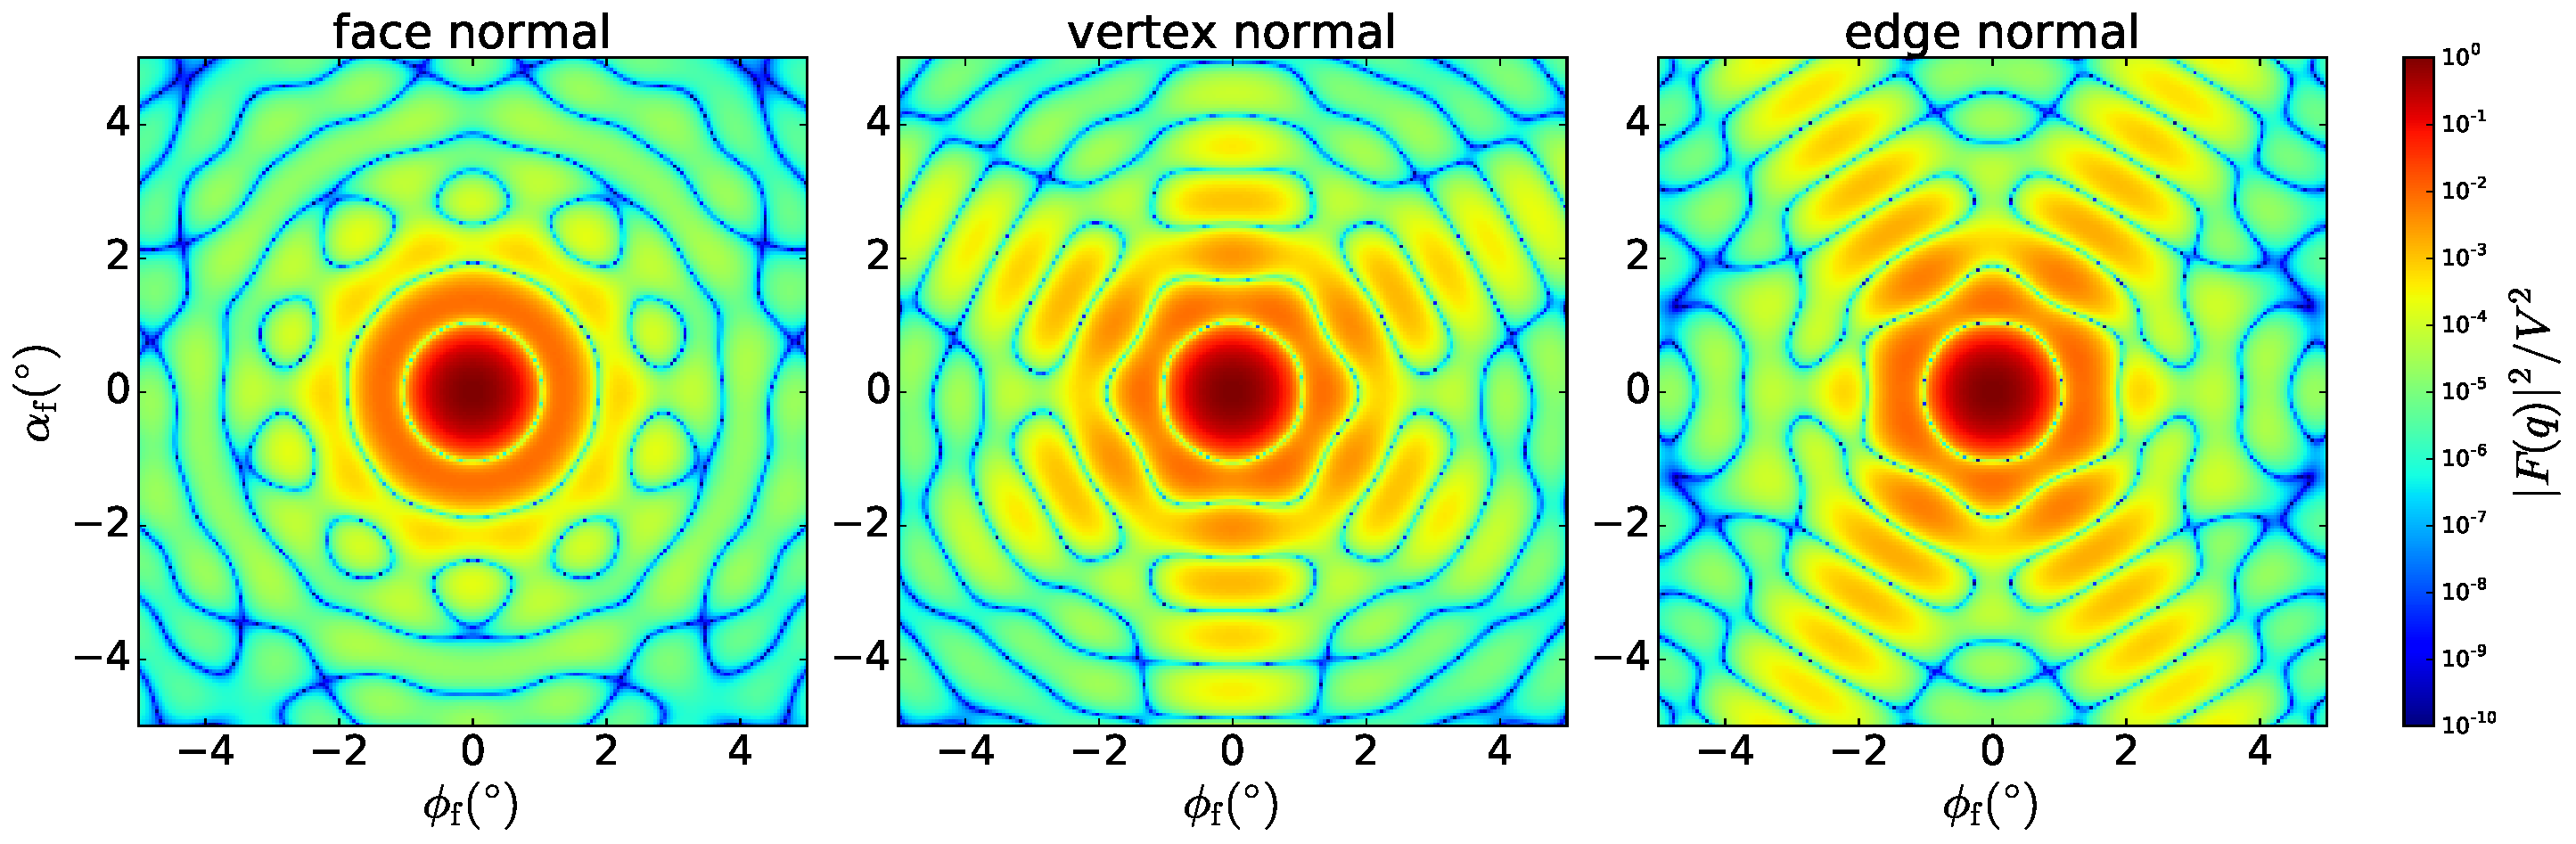
\includegraphics[width=\textwidth]{fig/ff2/ff_Dodecahedron_sym.pdf}
\end{center}
\caption{Normalized intensity $|F|^2/V^2$,
computed with $a=3.2$~nm,
for three orientations of high symmetry:
$x$ axis perpendicular to a polygonal face;
vertex on the $x$ axis;
edge in the $xy$ plane and perpendicular to the $x$ axis.}
\end{figure}

\begin{figure}[H]
\begin{center}
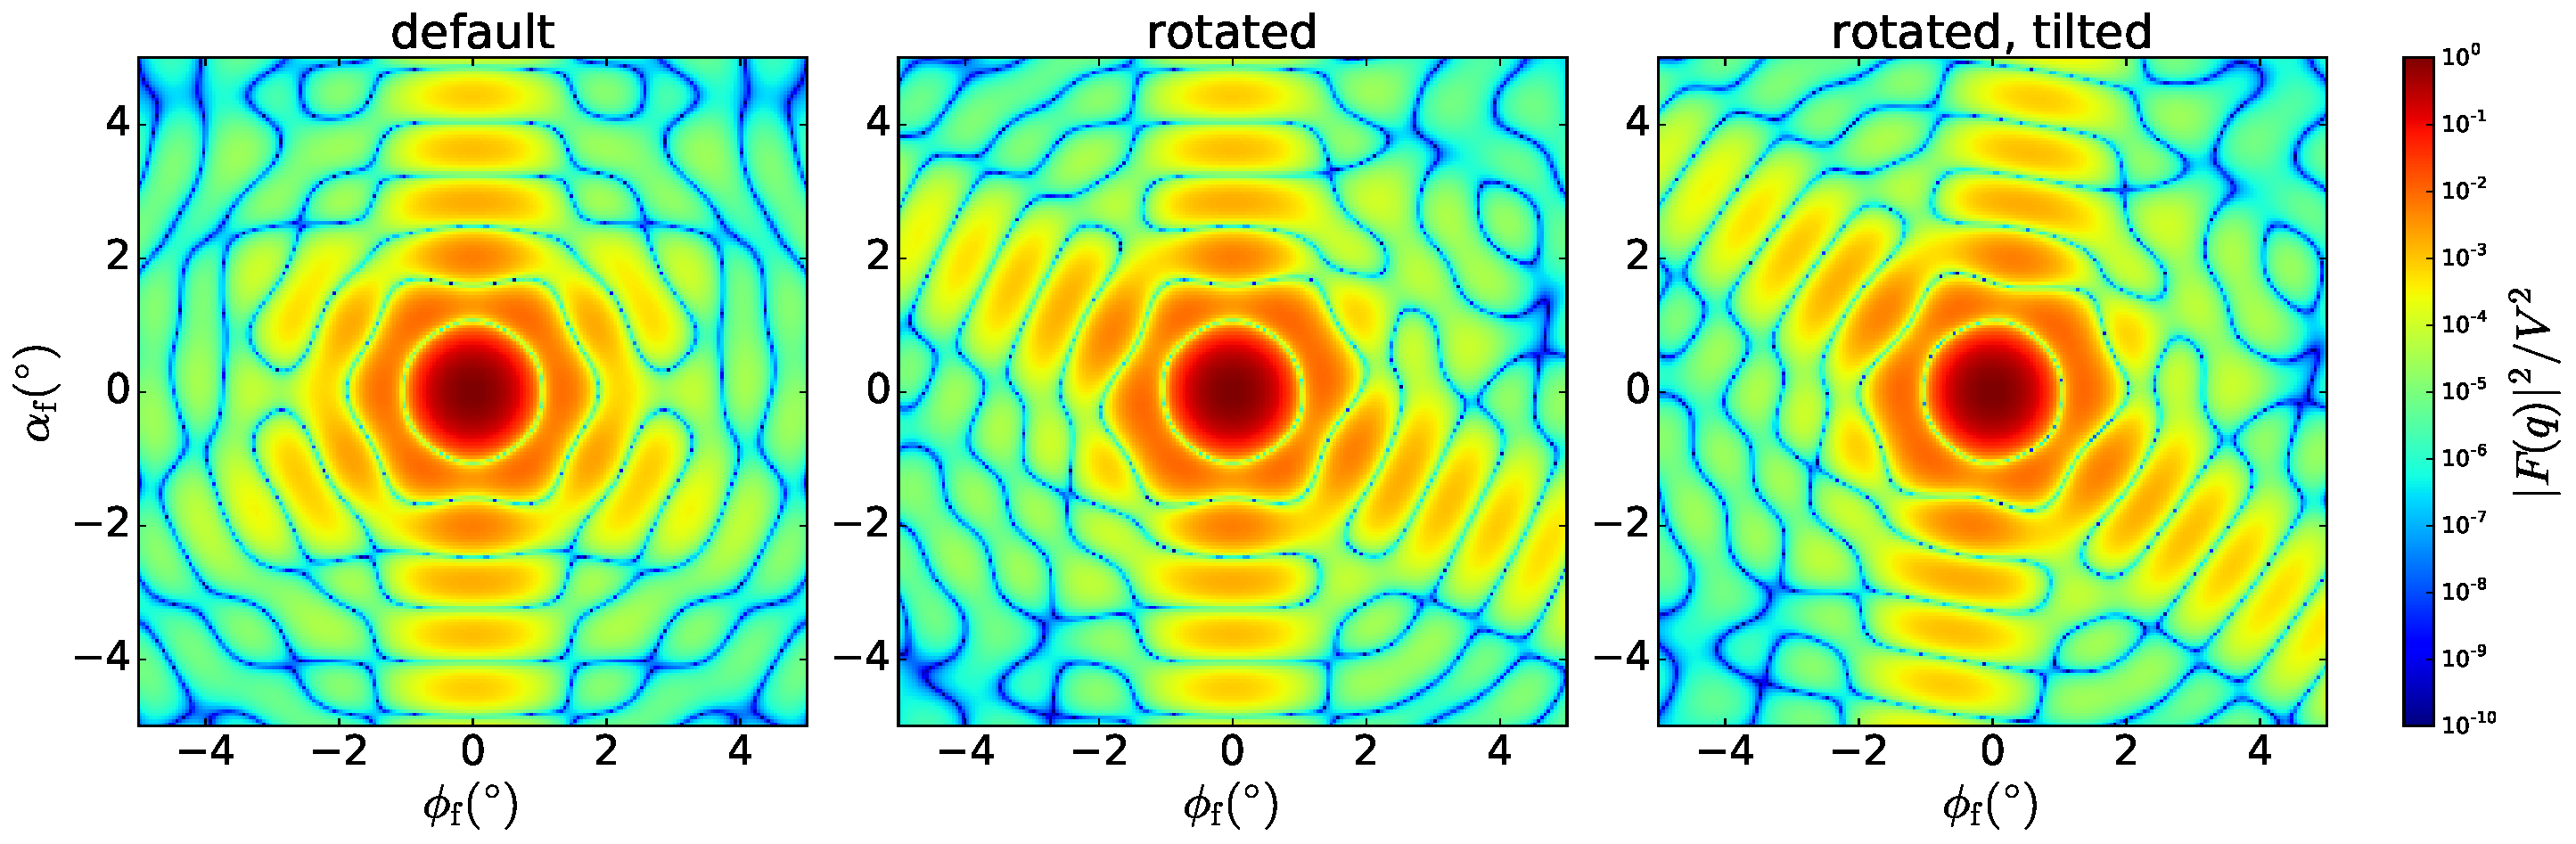
\includegraphics[width=\textwidth]{fig/ff2/ff_Dodecahedron_asy.pdf}
\end{center}
\caption{Normalized intensity $|F|^2/V^2$,
computed with $a=3.2$~nm,
for three orientations of decreasing symmetry:
base pentagon in $xy$ plane and pointing in $x$ direction;
rotated by $13^\circ$ around the $z$ axis;
ditto, and tilted by $9^\circ$ around the $x$ axis.}
\end{figure}

\paragraph{History}\strut\\
New in \BornAgain-1.6,
based on the generic form factor of the polyhedron~\cite{ba:ffp}.


%===============================================================================
\ffsection{EllipsoidalCylinder} \label{SEllipsoidalCylinder}
%===============================================================================
  \index{Ellipsoidal cylinder (form factor)}
  \index{Cylinder (form factor)!ellipsoidal}
  \index{FormFactorEllipsoidalCylinder@\Code{FormFactorEllipsoidalCylinder}}

\paragraph{Real-space geometry}\strut\\

\begin{figure}[H]
\hfill
\subfigure[Perspective]{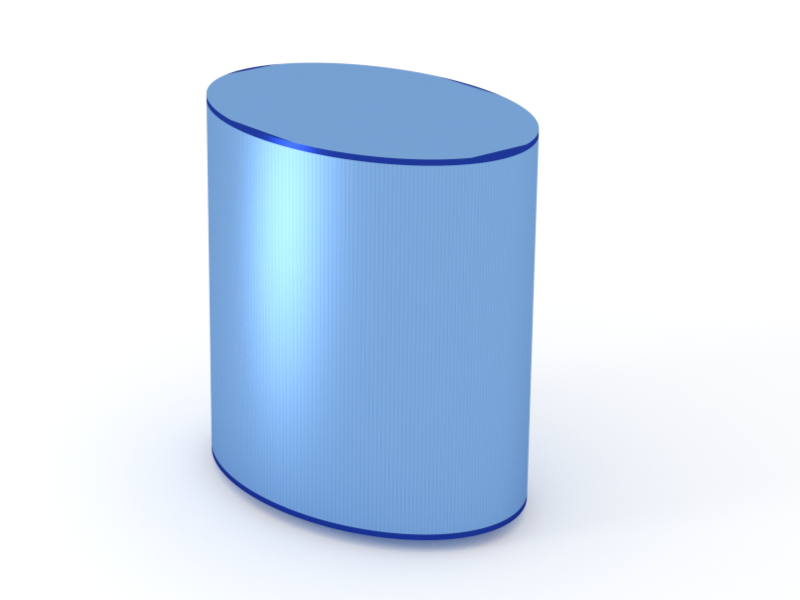
\includegraphics[width=.24\textwidth]{fig/blue/EllipsoidalCylinder3d.png}}
\hfill
\subfigure[Top view]{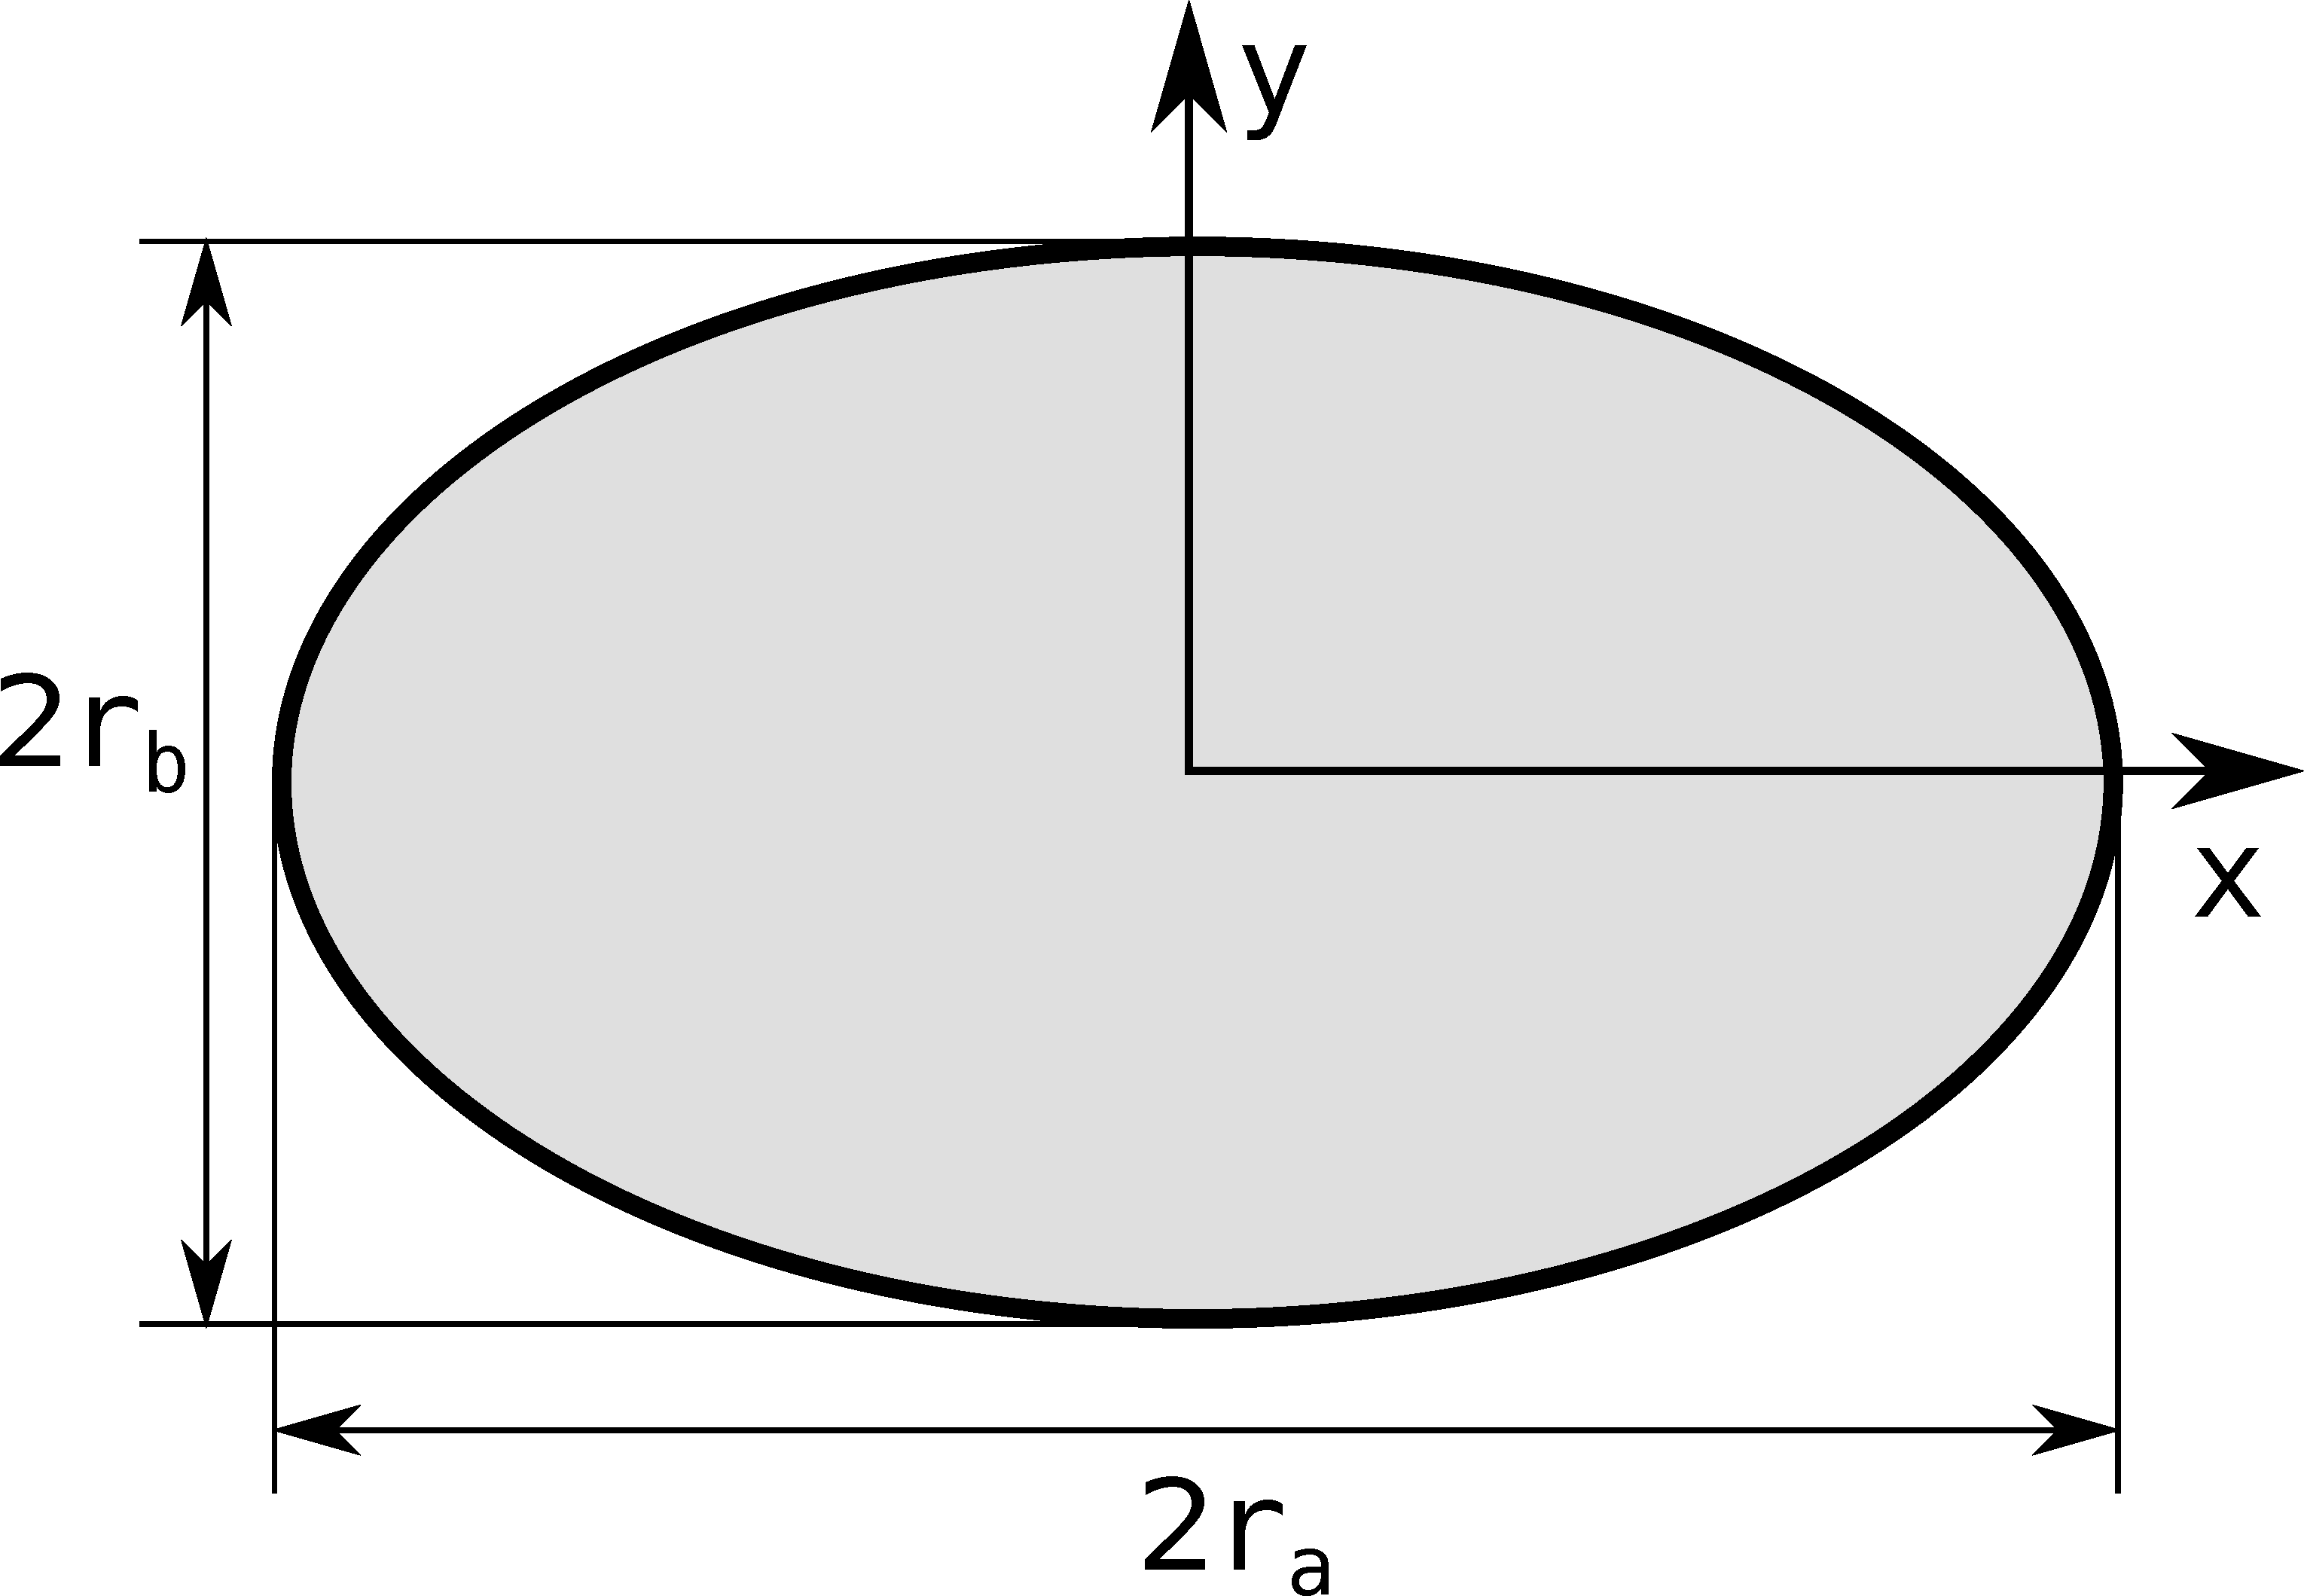
\includegraphics[width=.30\textwidth]{fig/cuts/EllipsoidalCylinder2dxy.pdf}}
\hfill
\subfigure[Side view]{\raisebox{4mm}{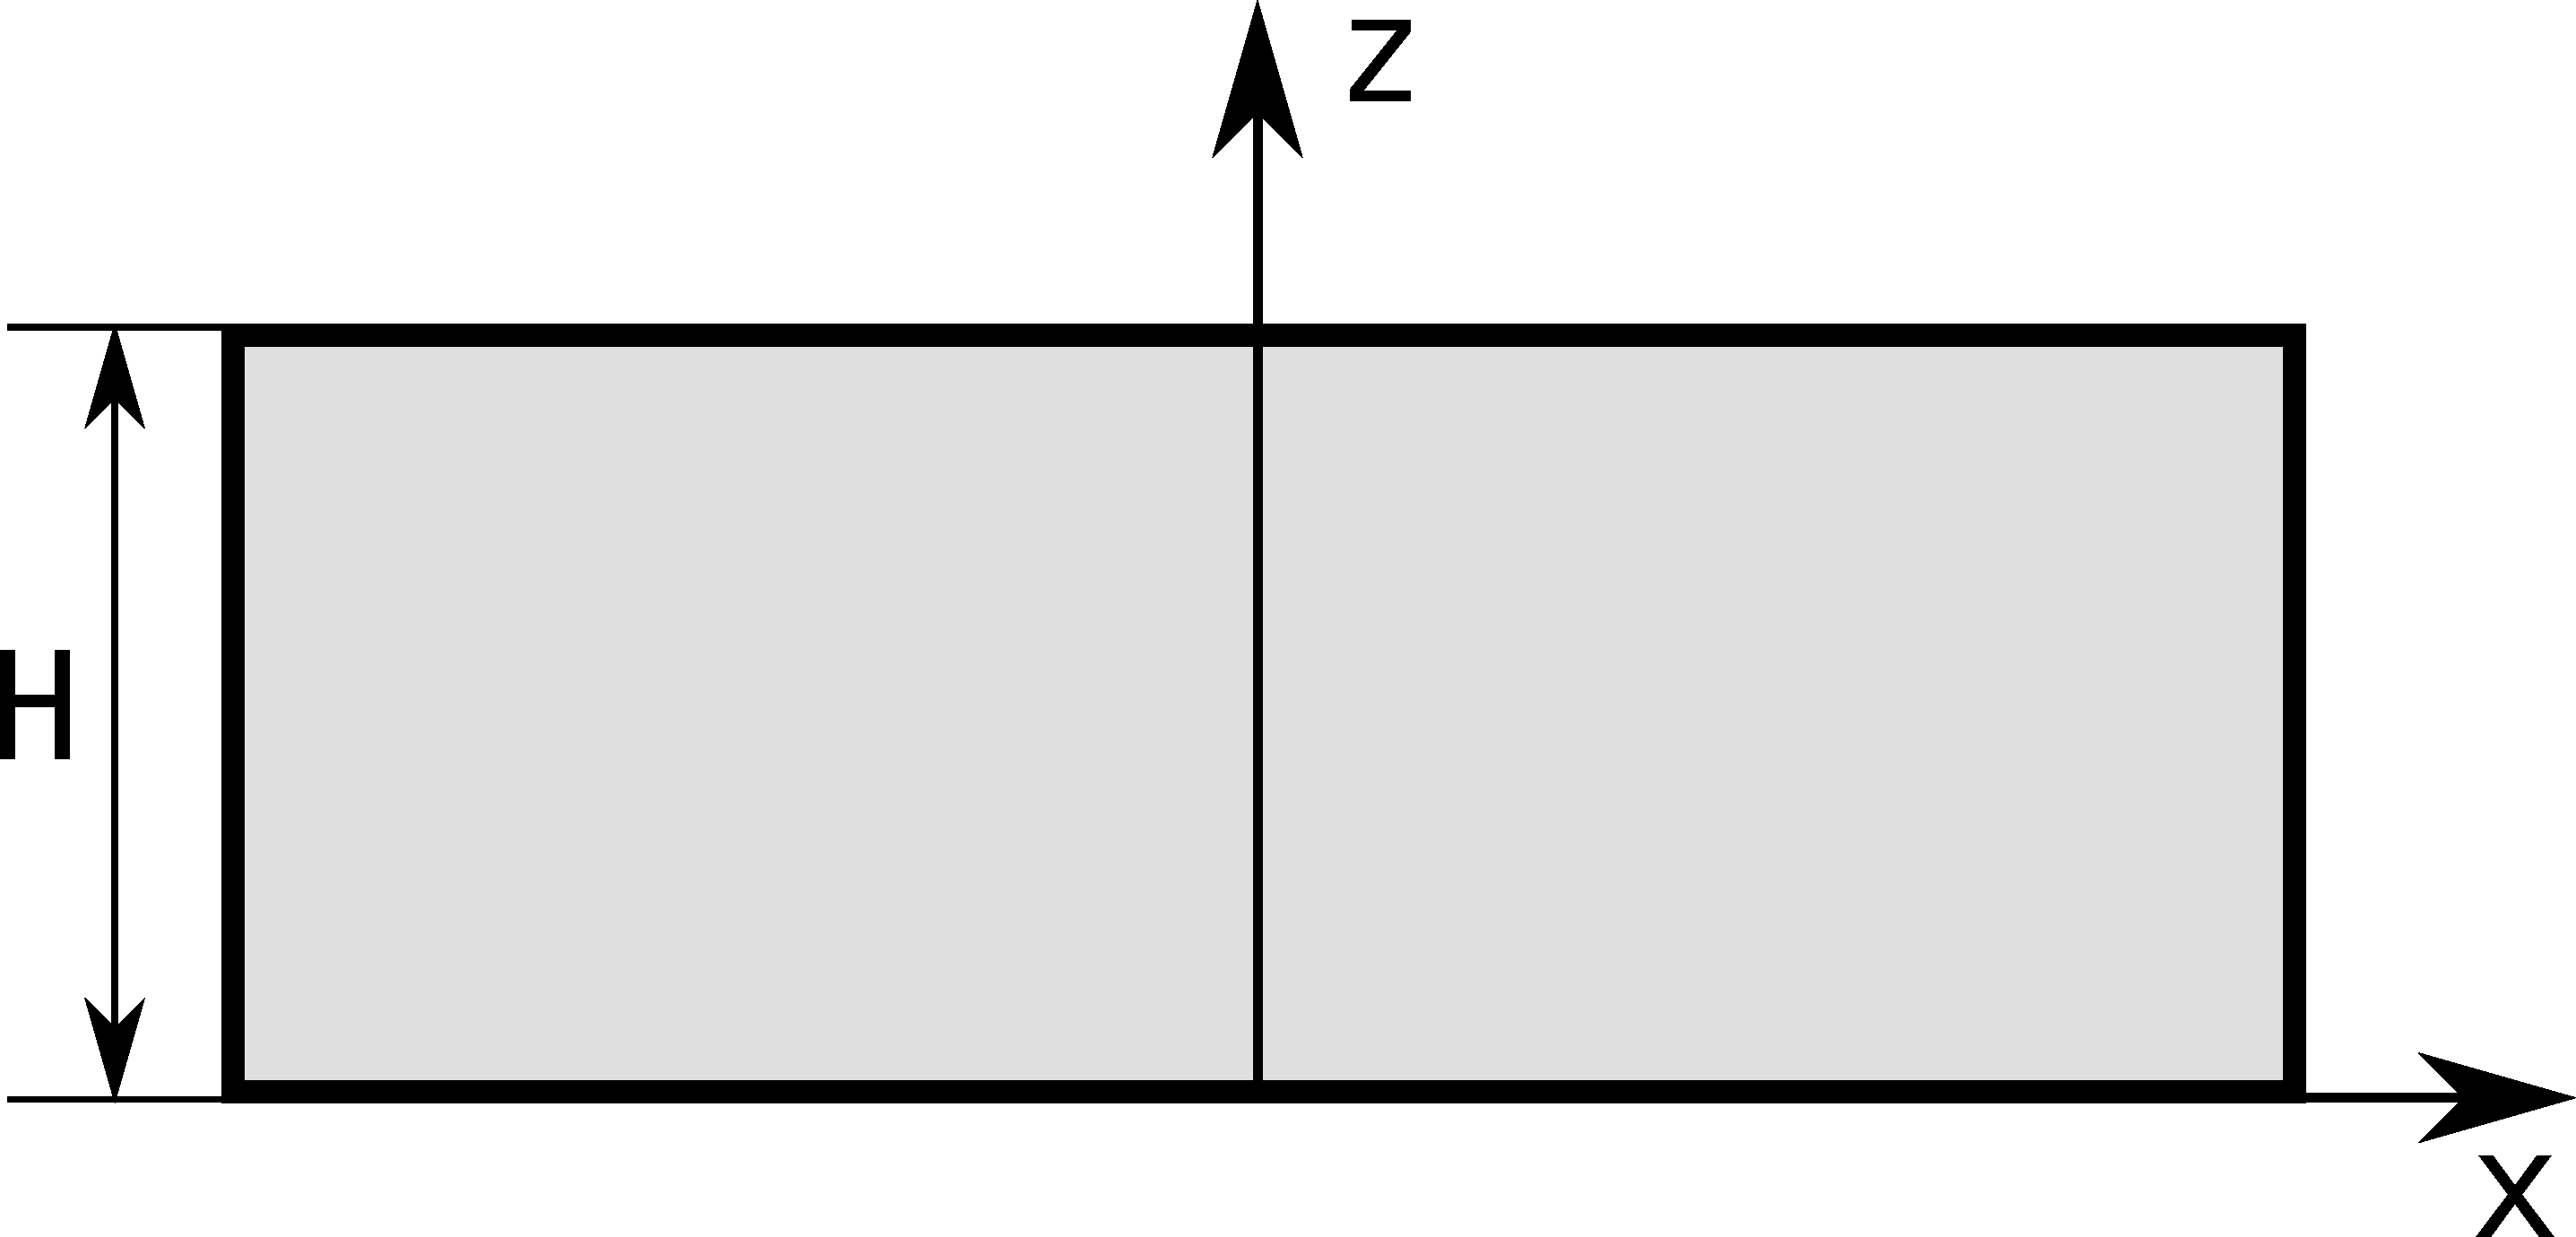
\includegraphics[width=.30\textwidth]{fig/cuts/EllipsoidalCylinder2dxz.pdf}}}
\hfill
\caption{A upright cylinder whose cross section is an ellipse.}
\end{figure}

\paragraph{Syntax and parameters}\strut\\[-2ex plus .2ex minus .2ex]
\begin{lstlisting}
  FormFactorEllipsoidalCylinder(radius_a, radius_b, height)
\end{lstlisting}
with the parameters
\begin{itemize}
\item \texttt{radius\_a}, in $x$ direction, $R_a$,
\item \texttt{radius\_b}, in $y$ direction, $R_b$,
\item \texttt{height}, $H$.
\end{itemize}

\paragraph{Form factor, volume, horizontal section}\strut\\
Notation:
\begin{equation*}
  \gamma \coloneqq \sqrt{(q_x R_a)^2+(q_y R_b)^2}
\end{equation*}
Results:
\begin{equation*}
F = 2\pi R_a R_b H \exp\left(i\frac{q_z H}{2}\right)
   \sinc\left(\frac{q_z H}{2}\right) \frac{J_1(\gamma)}{\gamma},
\end{equation*}
\begin{equation*}
  V = \pi R_a R_bH,
\end{equation*}
\begin{equation*}
  S = R_a R_b.
\end{equation*}

\paragraph{Examples}\strut

\begin{figure}[H]
\begin{center}
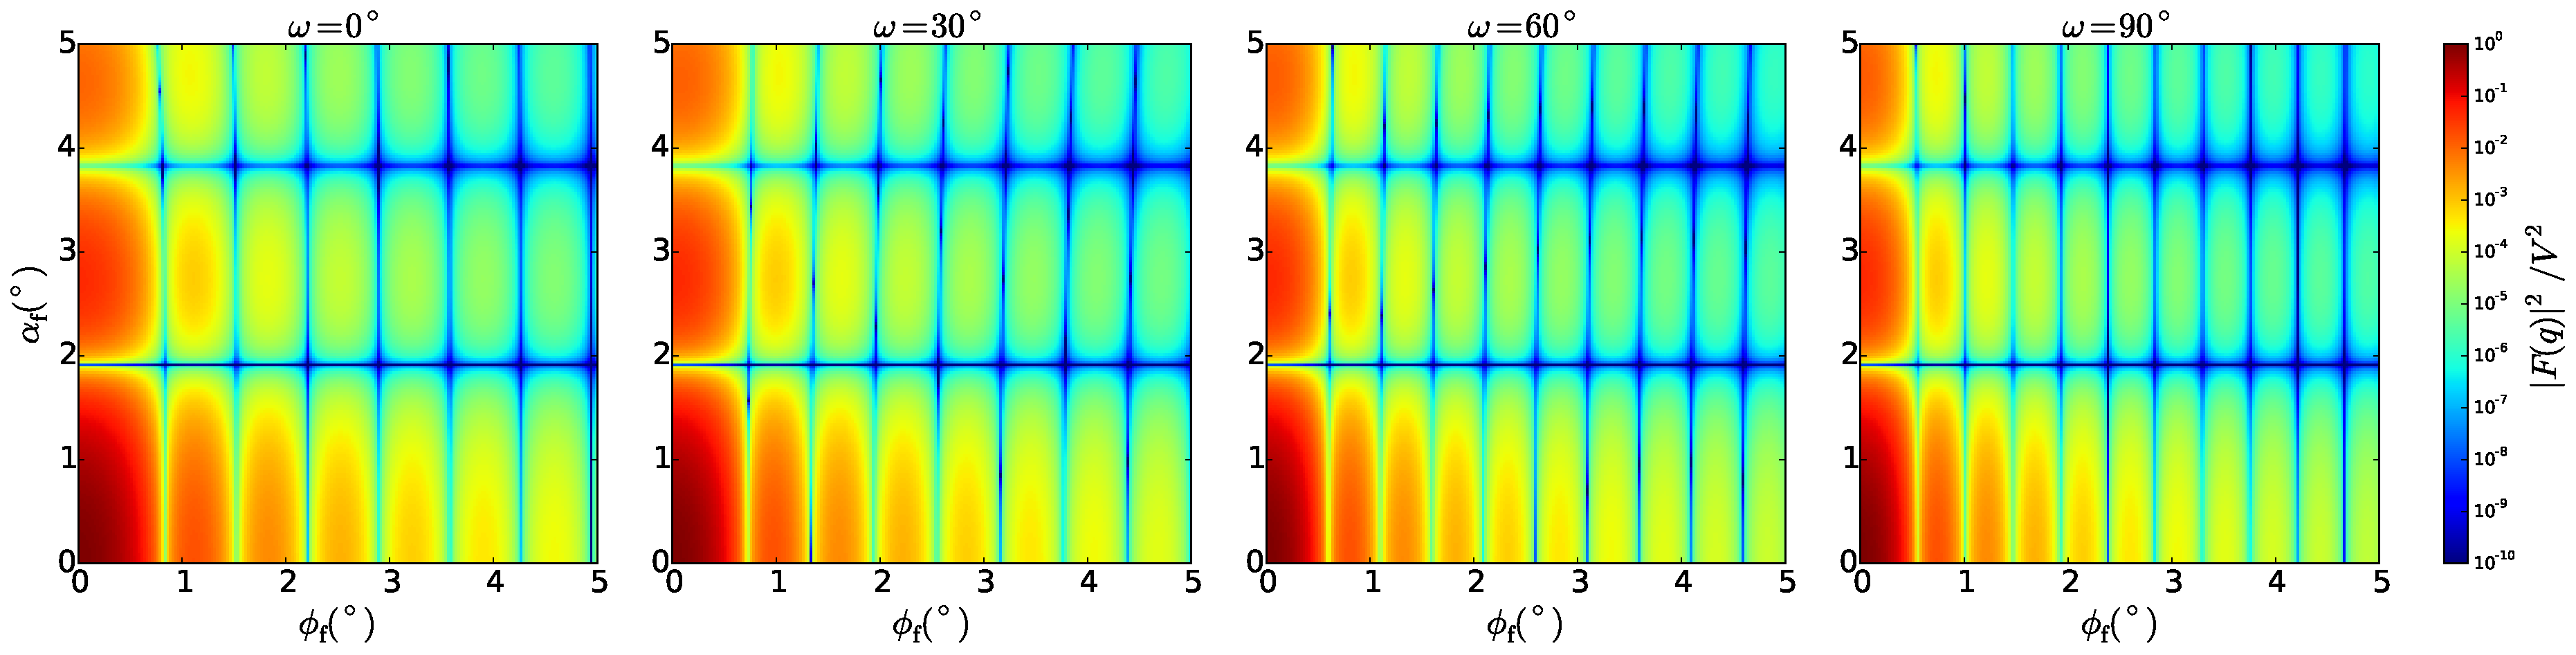
\includegraphics[width=\textwidth]{fig/ff2/ff_EllipsoidalCylinder.pdf}
\end{center}
\caption{Normalized intensity $|F|^2/V^2$,
computed with $R_a=6.3$~nm, $R_b=4.2$~nm and $H=3$~nm,
for four different angles~$\omega$ of rotation around the $z$ axis.}
\end{figure}

\paragraph{History}\strut\\
Agrees with the \IsGISAXS\ form factor
\E{Ellipsoid} \cite[Eq.~2.41, wrongly labeled in Fig.~2.4]{Laz08}
or \E{Ellipsoidal Cylinder} \cite[Eq.~224]{ReLL09}.


%===============================================================================
\ffsection{FullSphere} \label{SFullSphere}
%===============================================================================
  \index{Full sphere (form factor)}
  \index{Sphere (form factor)}
  \index{FormFactorFullSphere@\Code{FormFactorFullSphere}}

\paragraph{Real-space geometry}\strut\\

\begin{figure}[H]
\hfill
\subfigure[Perspective]{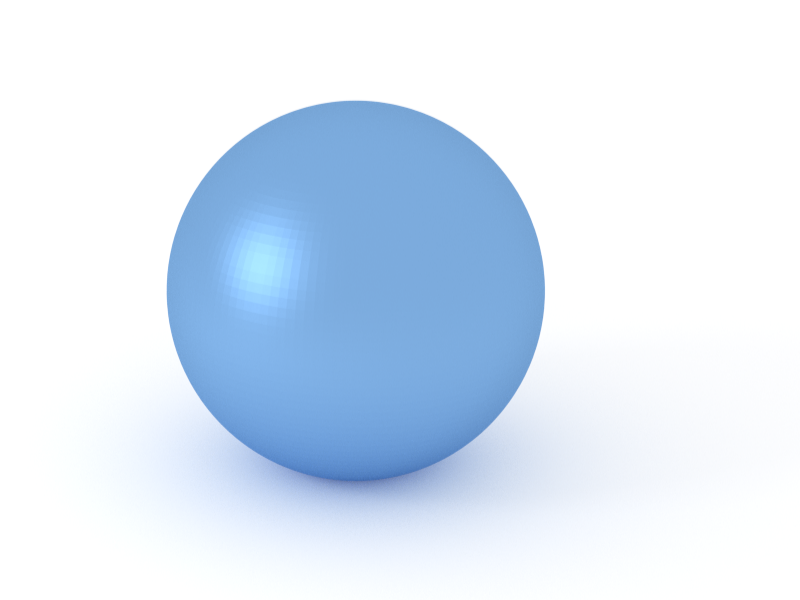
\includegraphics[width=.24\textwidth]{fig/blue/FullSphere3d.png}}
\hfill
\subfigure[Top view]{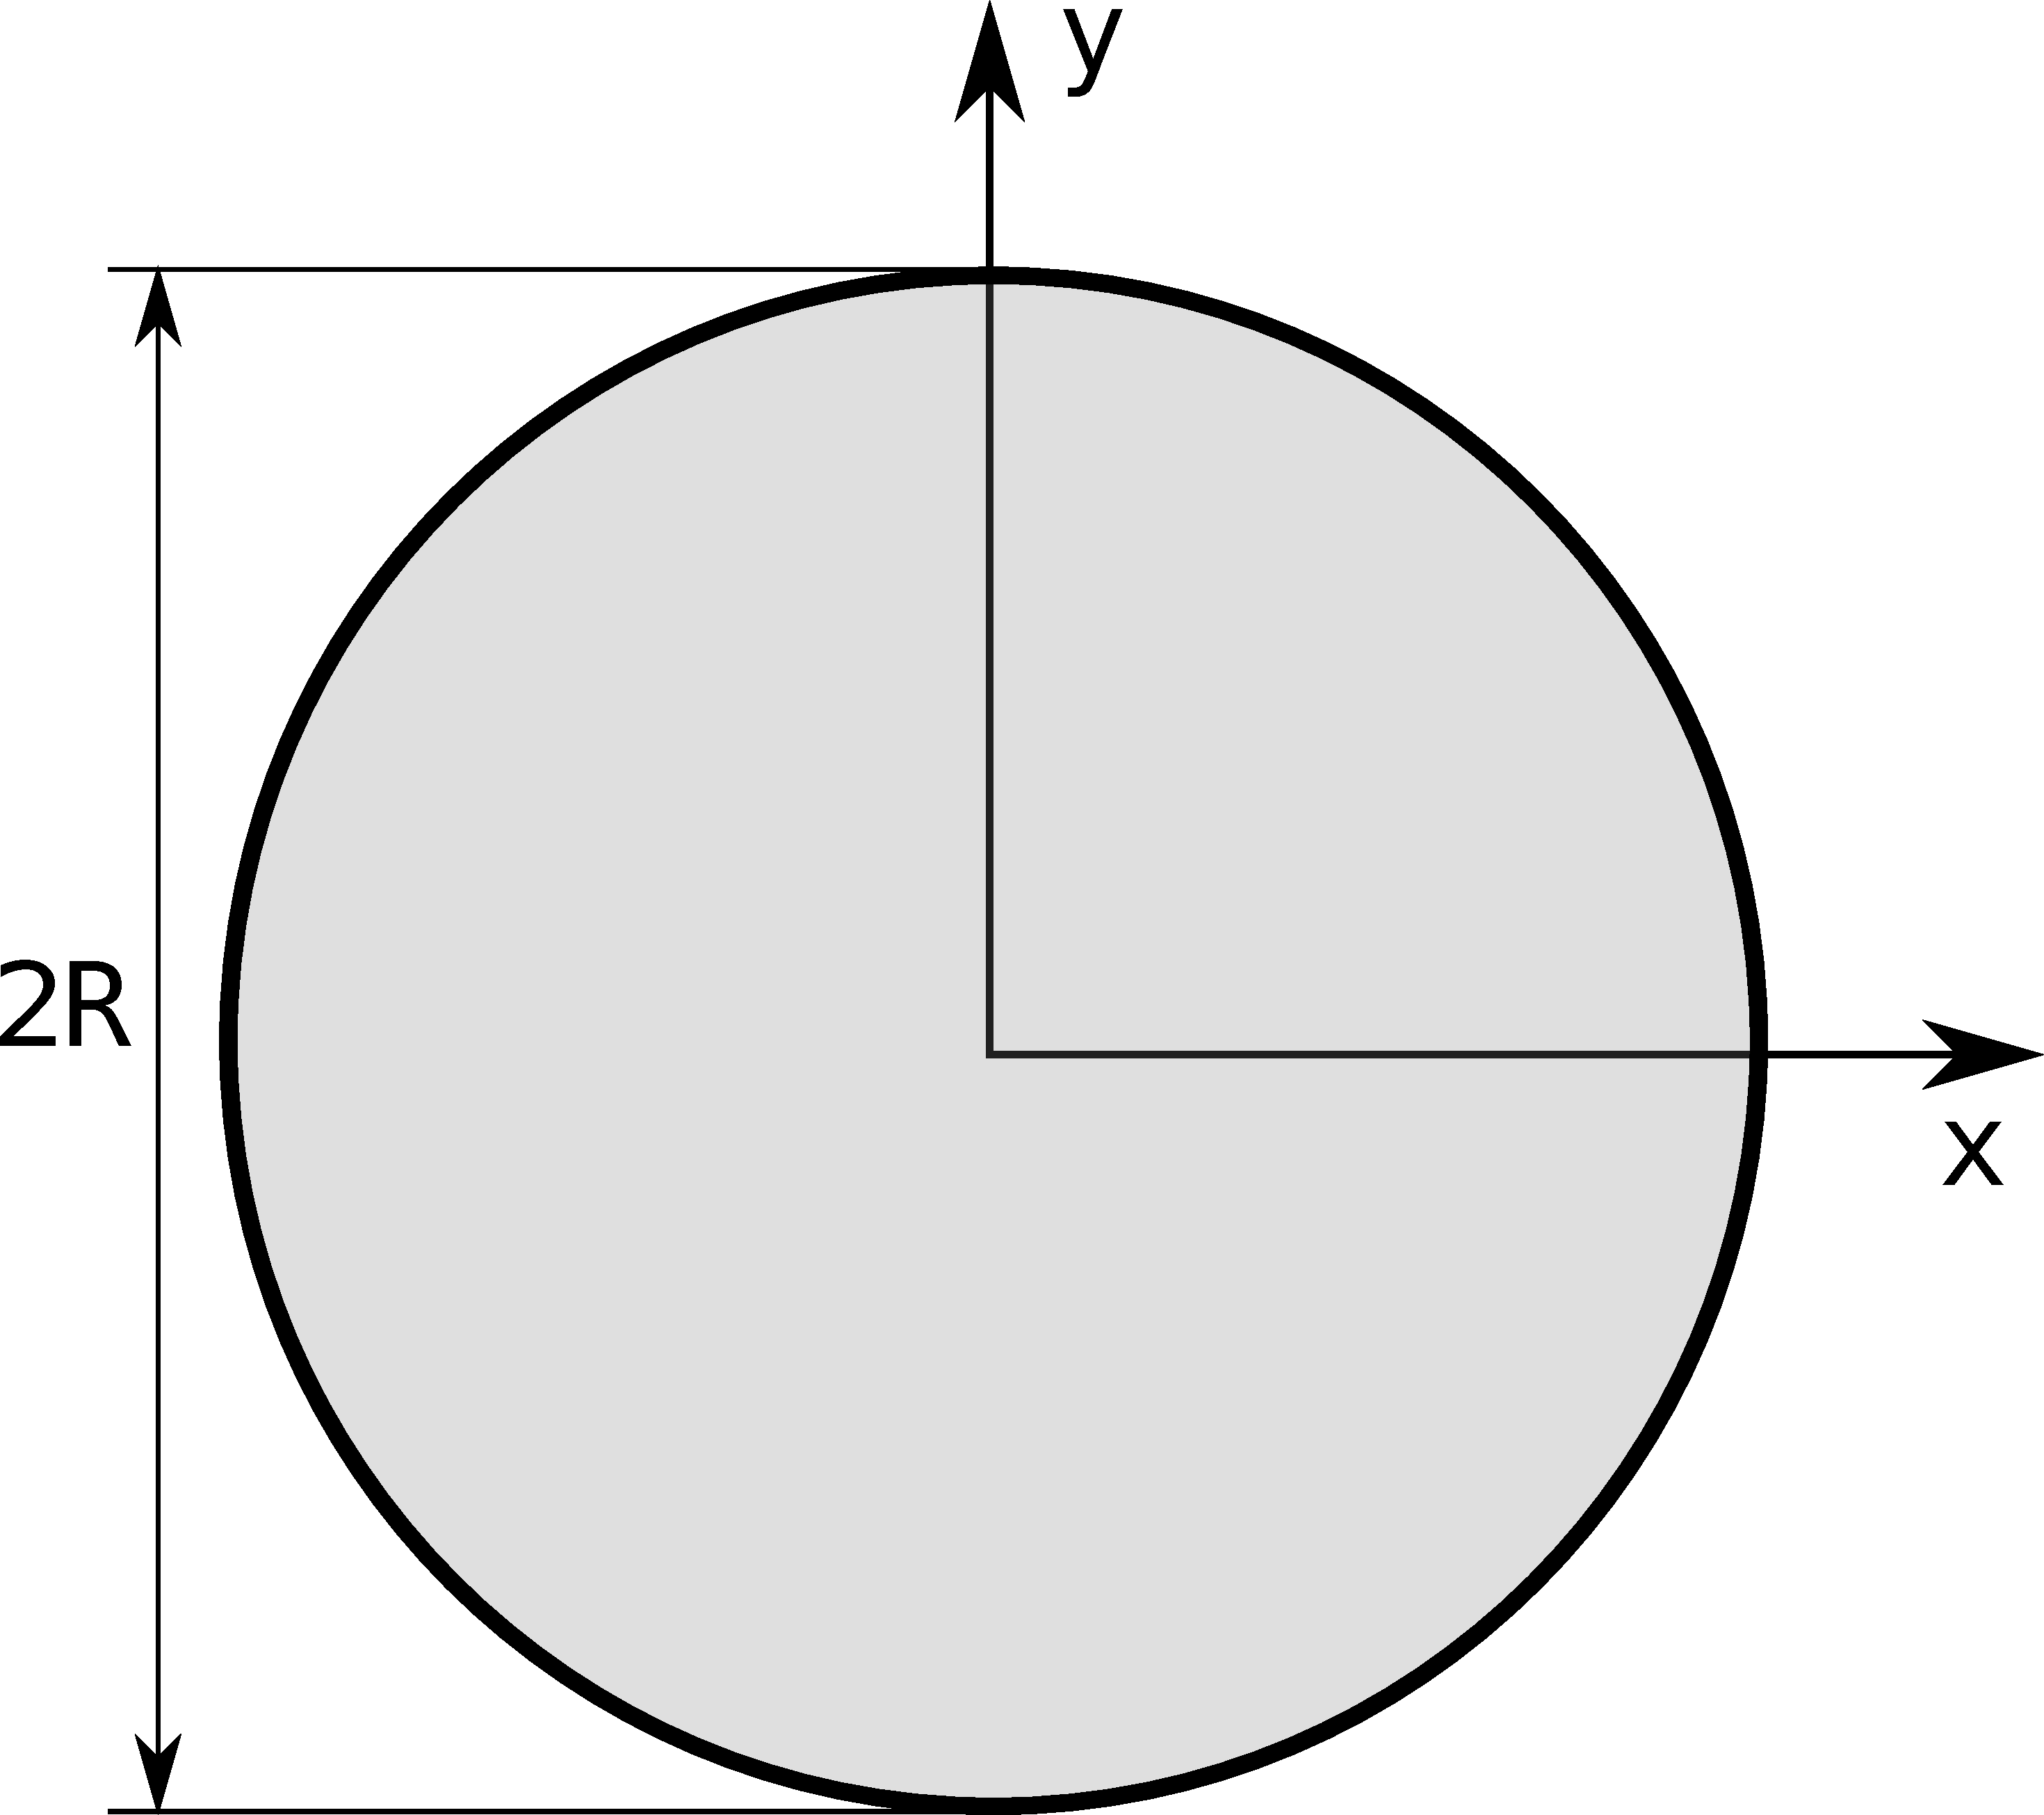
\includegraphics[width=.30\textwidth]{fig/cuts/FullSphere2dxy.pdf}}
\hfill
\subfigure[Side view]{\raisebox{-2mm}{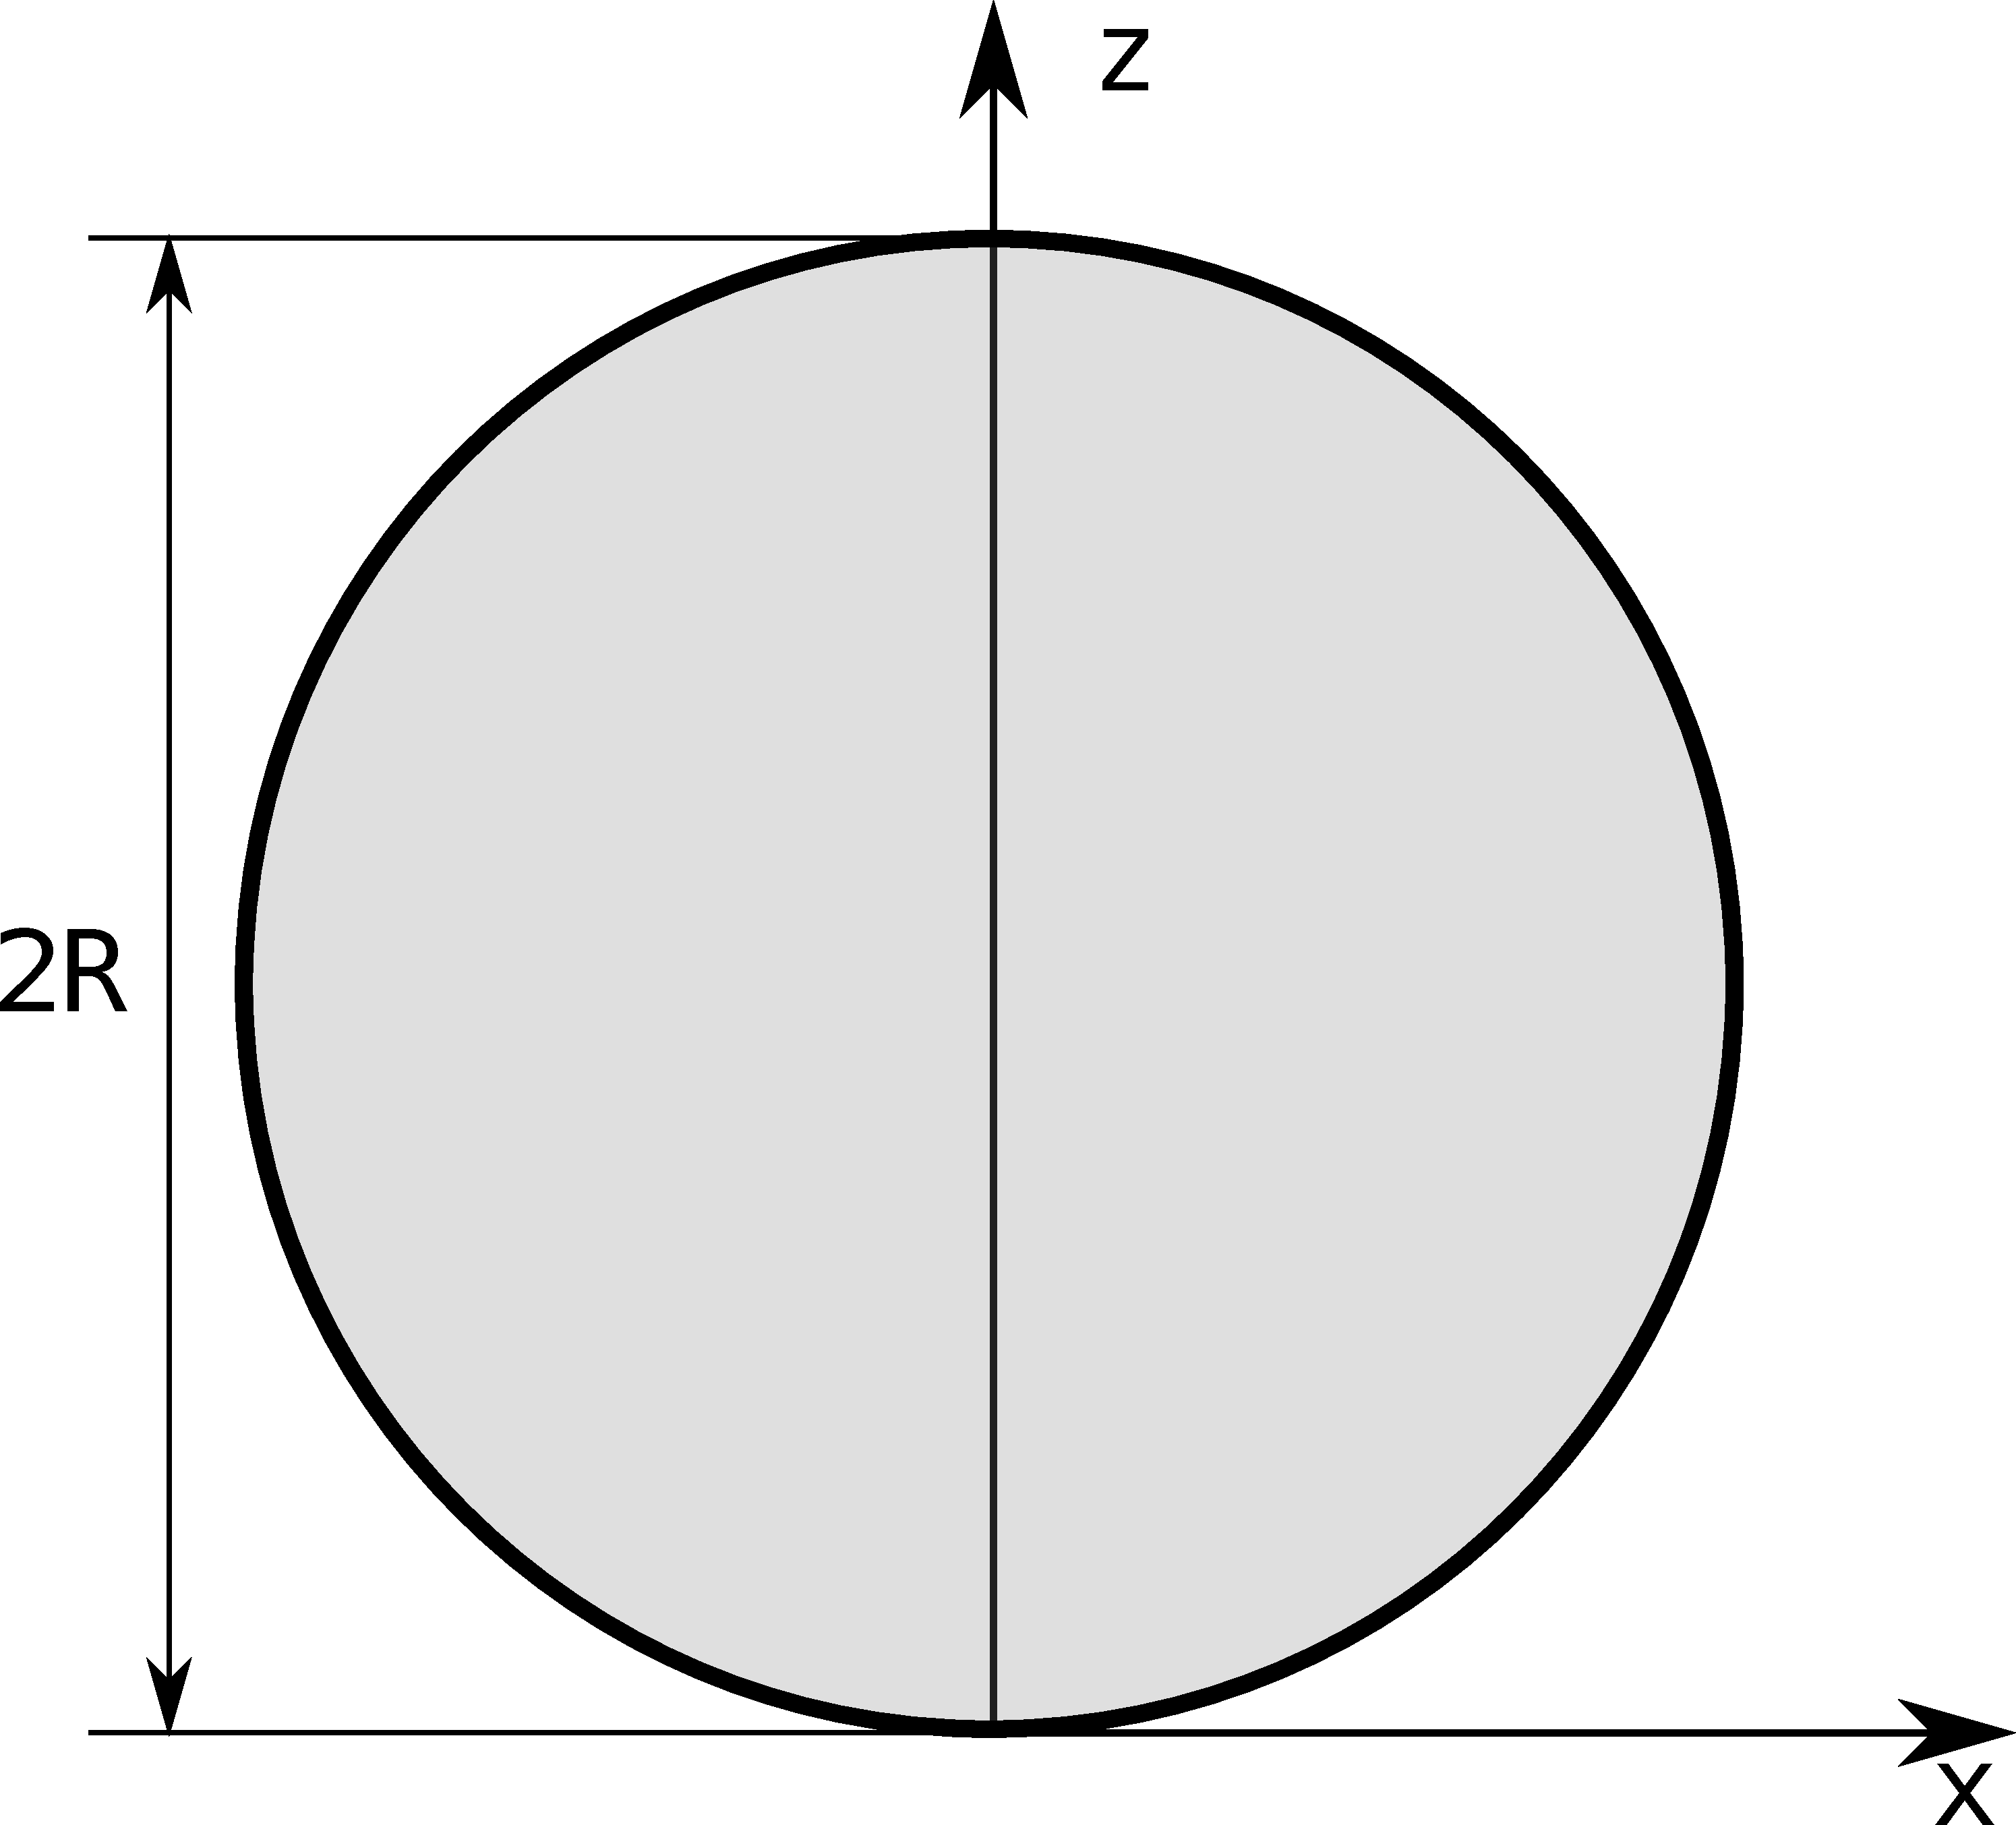
\includegraphics[width=.30\textwidth]{fig/cuts/FullSphere2dxz.pdf}}}
\hfill
\caption{A full sphere.}
\end{figure}

\FloatBarrier

\paragraph{Syntax and parameters}\strut\\[-2ex plus .2ex minus .2ex]
\begin{lstlisting}
  FormFactorFullSphere(radius)
\end{lstlisting}
with the parameter
\begin{itemize}
\item \texttt{radius}, $R$.
\end{itemize}

\paragraph{Form factor, volume, horizontal section}\strut\\
Notation:
\begin{equation*}
  q \coloneqq \sqrt{q_x^2+q_y^2+q_z^2}.
\end{equation*}
Note that this does \E{not} involve the sesquilinear product
$|q_x|^2=q_x^* q_x$ but the plain product $q_xq_x$ of complex numbers
(and analogous for~$q_y$, $q_z$).
\begin{equation*}
F = \frac{4\pi}{q^3} \exp(iq_z R)\left[\sin(qR) - qR \cos(qR)\right],
\end{equation*}
\begin{equation*}
  V = \dfrac{4\pi}{3}R^3,
\end{equation*}
\begin{equation*}
  S= \pi R^2.
\end{equation*}

\paragraph{Example}\nopagebreak\strut\nopagebreak

\begin{figure}[H]
\begin{center}
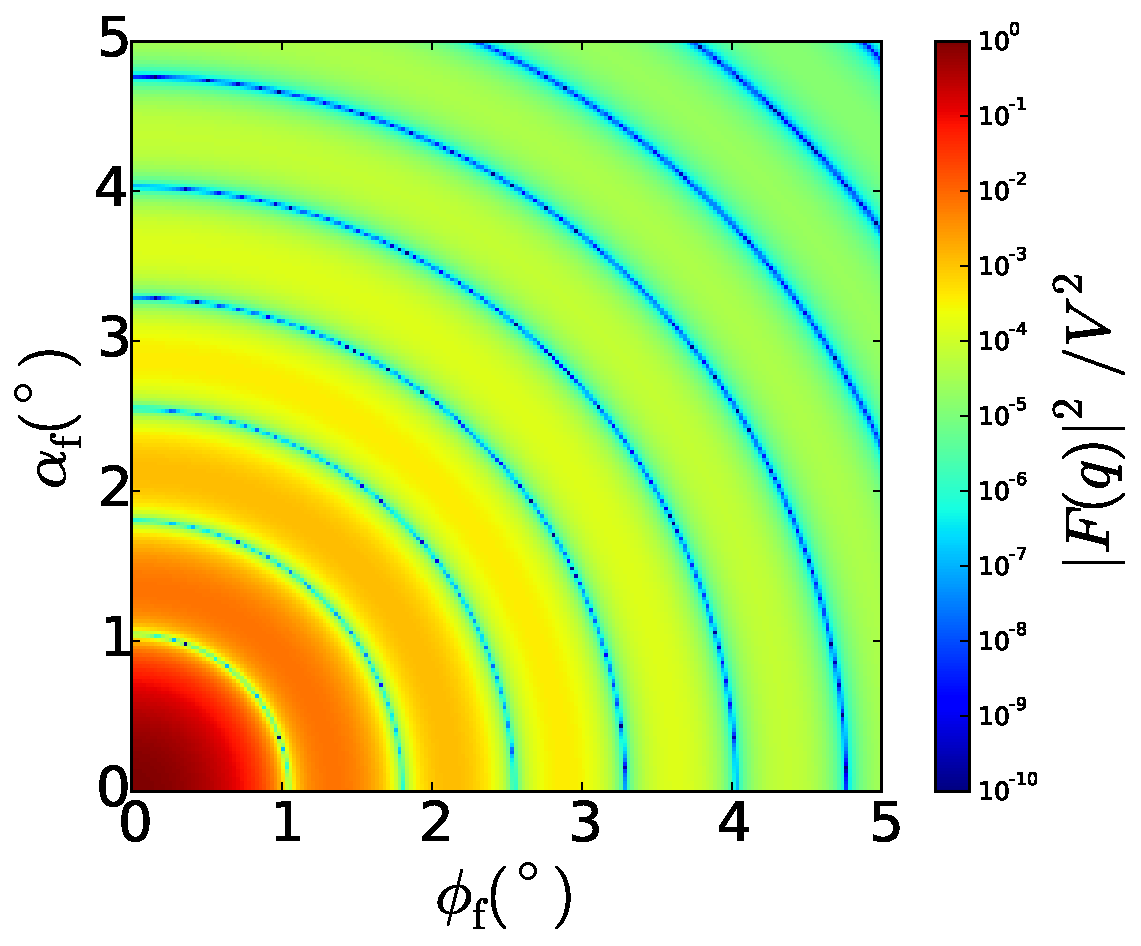
\includegraphics[width=0.5\textwidth]{fig/ff2/ff_FullSphere.pdf}
\end{center}
\caption{Normalized intensity $|F|^2/V^2$,
computed with $R=3.9$~nm.}
\end{figure}

\paragraph{History and Derivation}\strut\\
For real wave vectors, this form factor is well known;
it goes back at least to Lord Rayleigh.
In \IsGISAXS, it has been implemented as form factor \E{Full sphere}
\cite[Eq.~2.36]{Laz08} \cite[Eq.~226]{ReLL09},
allowing for complex wavevectors.
Since it is not obvious that Rayleigh's formula also holds for complex~$\q$,
let us outline a derivation
(if you know a more elegant one, we would like to hear).

If the origin is at the center of the sphere, then the form factor is
\begin{equation}
I(\q,R)
 = \int_0^R\d r\, r^2\int_0^{\pi}\d\theta\,\sin\theta\int_0^{2\pi}\d\varphi
  \:\e^{i\q\r}
\end{equation}
with $\q\r
= q_x r\sin\theta\cos\varphi + q_y r\sin\theta\sin\varphi + q_z r\cos\theta$.
For the integration over $\varphi$,
see \cref{SCylinder} on the form factor of a cylinder:
\begin{equation}
  I(\q,R)
  = 2\pi \int_0^R \d r\,r^2 \int_0^{\pi} \d\theta\, \sin\theta
   \exp\left(i q_z \cos \theta\right) J_0\left(q_\parallel r\sin \theta\right)
\end{equation}
with $q_{\parallel}=\sqrt{q_x^2+q_y^2}$.
By symmetry, the imaginary part is zero,
so that the exponential reduces to a cosine:
\begin{equation}
  I(\q,R)
  = 2\pi \int_0^R \d r\,r^2 \int_0^{\pi} \d\theta\, \sin\theta
   \cos\left(q_z \cos \theta\right) J_0\left(q_\parallel r\sin \theta\right).
\end{equation}
Expand the cosine and the Bessel function:
\begin{equation}
  I(\q,R)
  = 2\pi \int_0^R \d r\,r^2 \int_0^{\pi} \d\theta\, \sin\theta
    \sum_{j=0}^\infty (-)^j \frac{(q_zr\cos\theta)^{2j}}{(2j)!}\,
    \sum_{k=0}^{\infty} (-)^k \frac{(q_\parallel r \sin\theta)^{2k}}{4^k k!^2}.
\end{equation}
Sort by powers of $r$, and integrate:
\begin{equation}
  I(\q,R)
  = 2\pi \sum_{n=0}^\infty (-)^n \frac{R^{2n+3}}{2n+3} \sum_{k=0}^n
    \frac{{q_z}^{2n-2k}}{(2n-2k)!}\,\frac{{q_\parallel}^{2k}}{4^k k!^2} \zeta(k,n)
\end{equation}
with
\begin{equation}
  \zeta(k,n)
  \coloneqq \int_0^{\pi} \d\theta\, \sin\theta
  (\cos\theta)^{2n-2k}(\sin\theta)^{2k}.
\end{equation}
This integral \cite[no.\ 2.512.4]{GrRy07} yields
\begin{equation}
  \zeta(k,n)
  = \frac{2^{2k+1}(2n-2k)! n! k!}{(2n+1)!(n-k)!}.
\end{equation}
Hence
\begin{equation}\label{ESphereU}
  I(\q,R)
  = 4\pi \sum_{n=0}^\infty (-)^n \frac{R^{2n+3}}{(2n+3)(2n+1)!}
    \sum_{k=0}^n \frac{n!}{(n-k)!k!}{q_z}^{2n-2k}{q_\parallel}^{2k}.
\end{equation}
The inner sum happens to be the binomial expansion of
$q^{2n}=\left({q_z}^2+{q_\parallel}^2\right)^n$.
Therefore \cref{ESphereU} coincides with the series expansion of
\begin{equation}
  I(\q,R)
  = 4\pi q^{-3} \left( \sin(qR) - qR\cos(qR) \right),
\end{equation}
which is what we wanted to prove.

%===============================================================================
\ffsection{FullSpheroid} \label{SFullSpheroid}
%===============================================================================
  \index{Full spheroid (form factor)}
  \index{Spheroid (form factor)}
  \index{FormFactorFullSpheroid@\Code{FormFactorFullSpheroid}}

\paragraph{Real-space geometry}\strut\\

\begin{figure}[H]
\hfill
\subfigure[Perspective]{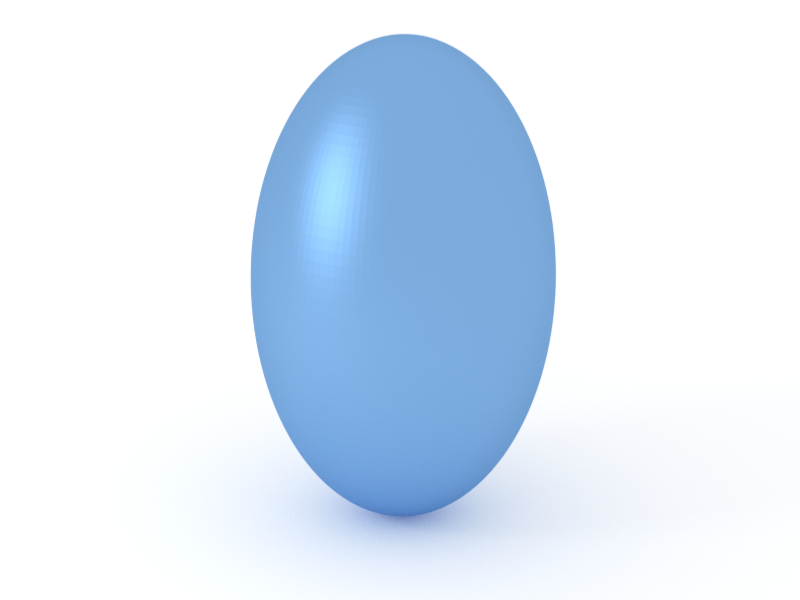
\includegraphics[width=.24\textwidth]{fig/blue/FullSpheroid3d.png}}
\hfill
\subfigure[Top view]{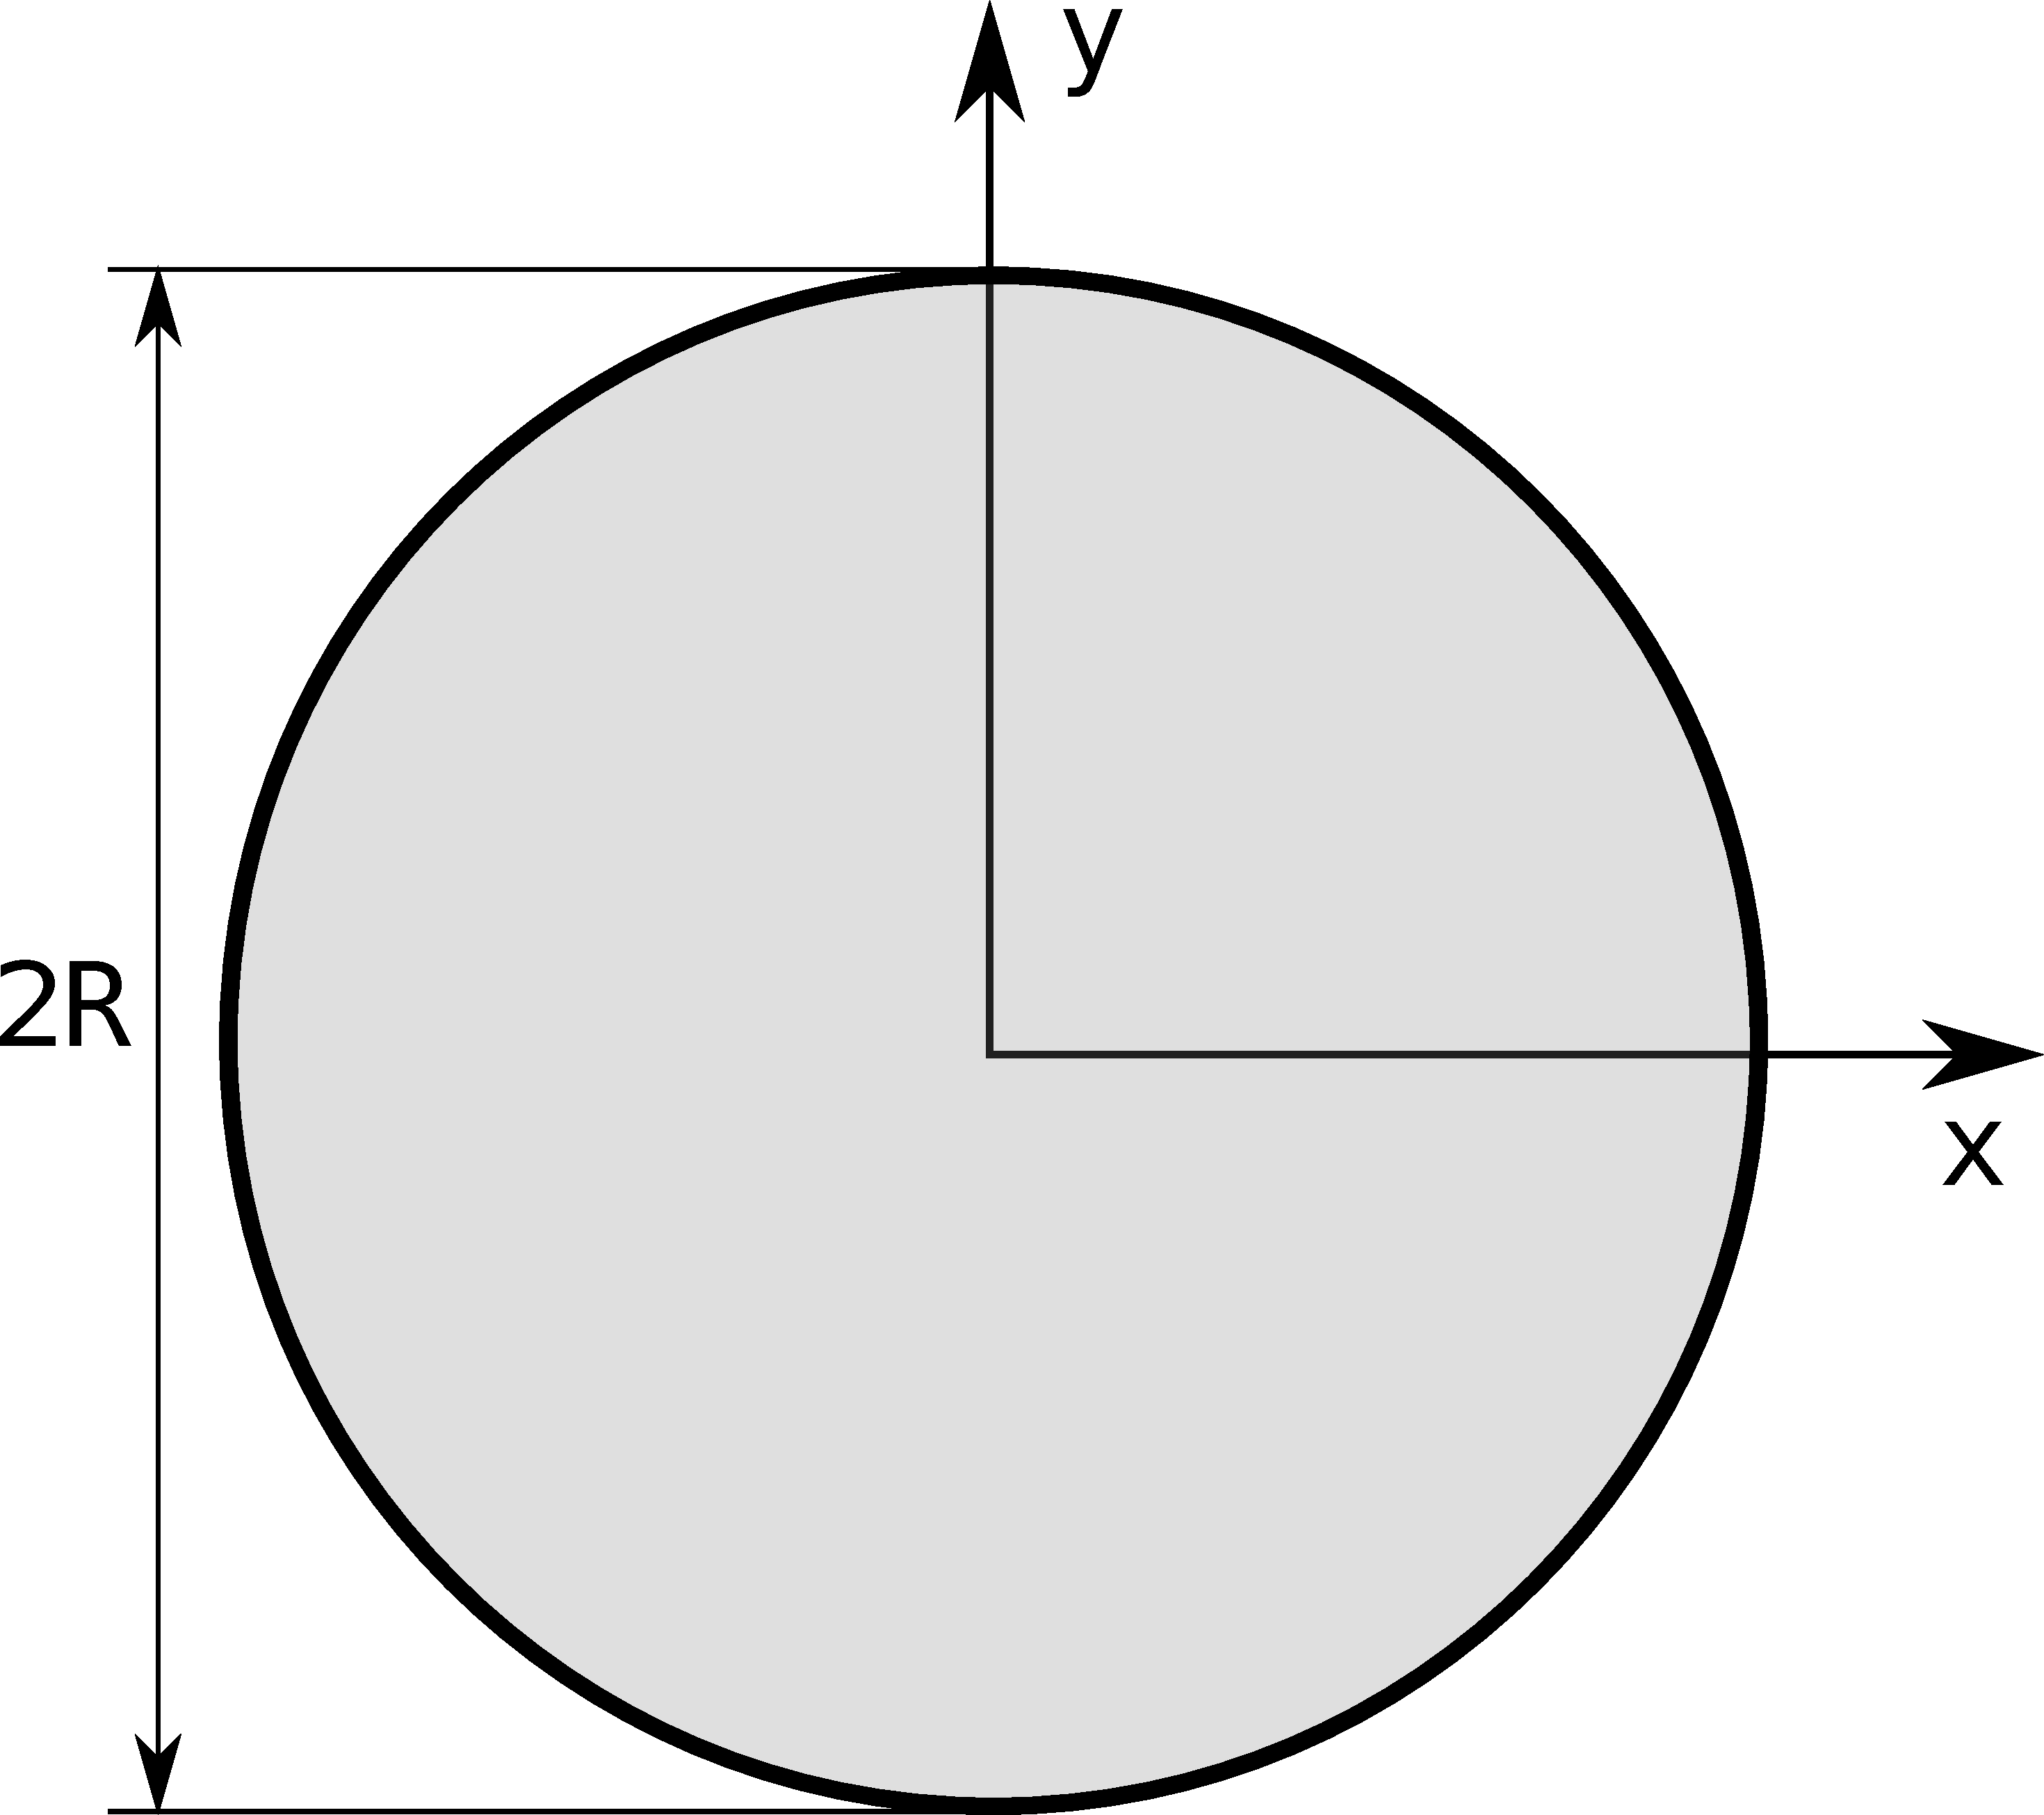
\includegraphics[width=.30\textwidth]{fig/cuts/FullSpheroid2dxy.pdf}}
\hfill
\subfigure[Side view]{\raisebox{-3mm}{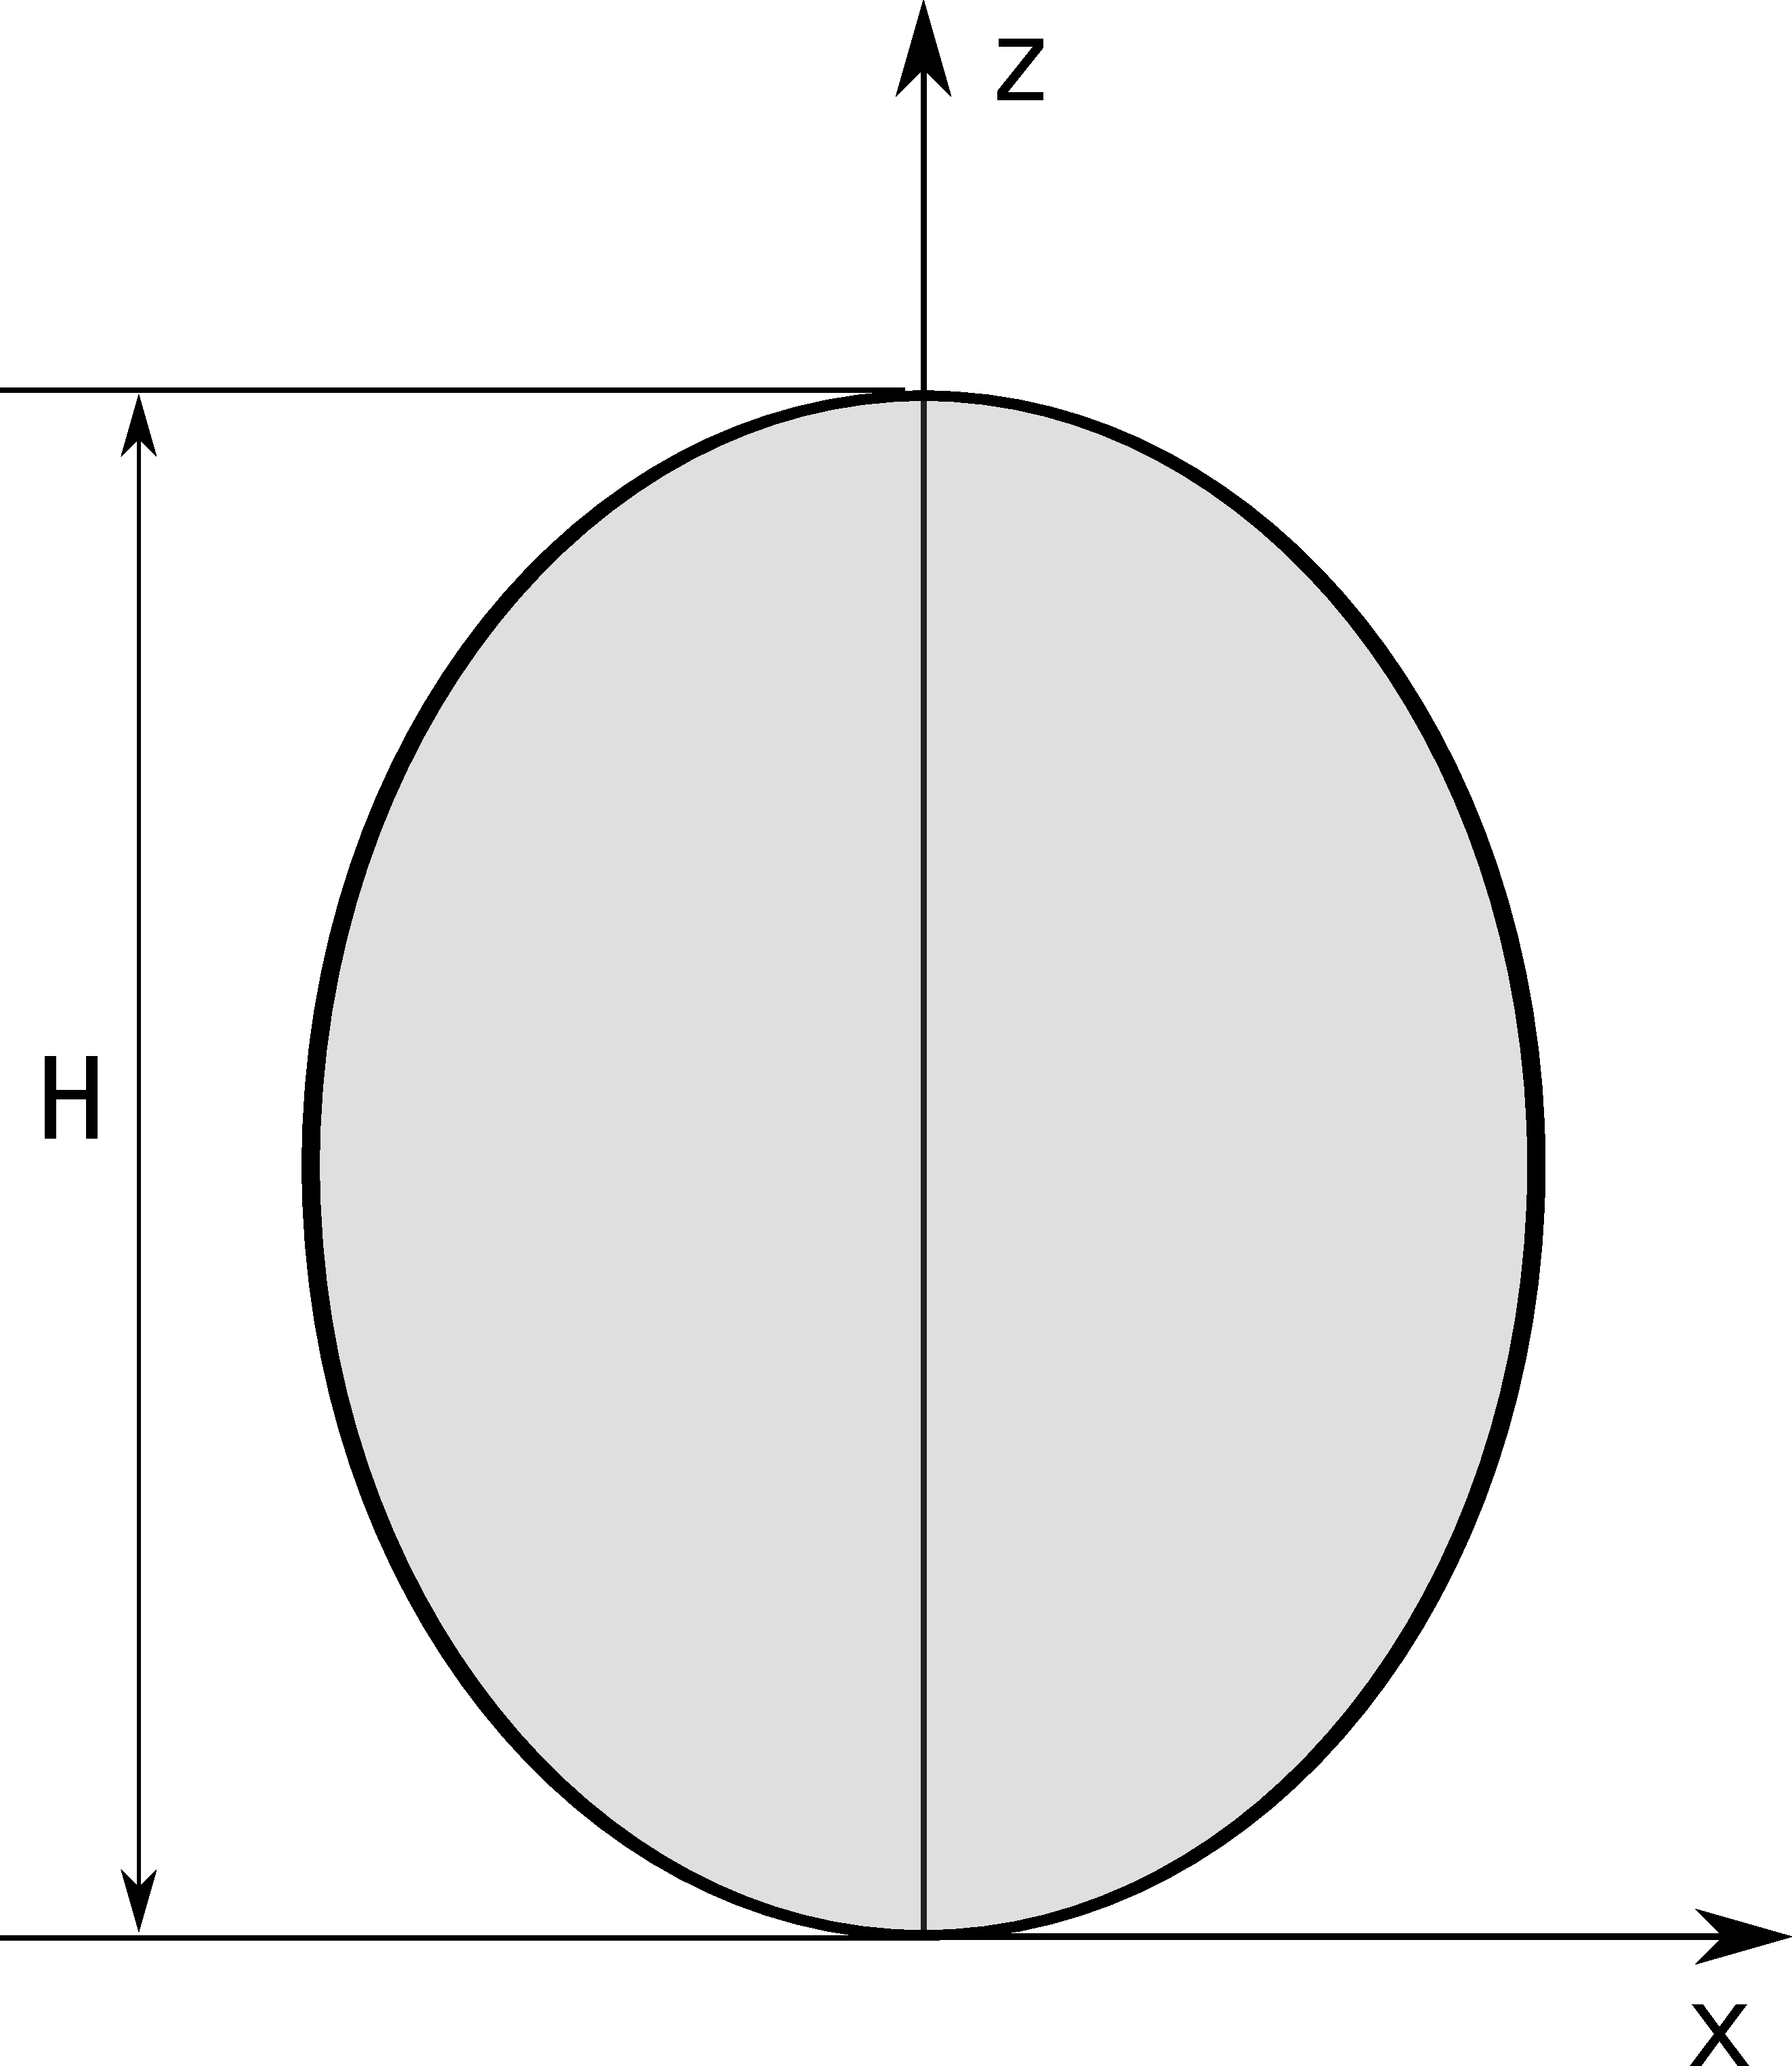
\includegraphics[width=.30\textwidth]{fig/cuts/FullSpheroid2dxz.pdf}}}
\hfill
\caption{A full spheroid, generated by rotating an ellipse around the vertical axis.}
\end{figure}

\FloatBarrier

\paragraph{Syntax and parameters}\strut\\[-2ex plus .2ex minus .2ex]
\begin{lstlisting}
  FormFactorFullSpheroid(radius,height)
\end{lstlisting}
with the parameters
\begin{itemize}
\item \texttt{radius}, $R$,
\item \texttt{height}, $H$.
\end{itemize}

\paragraph{Form factor, volume, horizontal section}\strut\\
Notation:
\begin{equation*}
 R_z \coloneqq R\sqrt{1-\frac{4z^2}{H^2}},\quad
 q_\plll \coloneqq \sqrt{q_x^2+q_y^2}.
\end{equation*}
Results:
\begin{equation*}
  F = 4\pi \exp(i q_z H/2) \int_0^{H/2} \!\d z\,
     R_z^2 \frac{J_1(q_{\parallel}R_z)}{q_{\parallel}R_z} \cos(q_z z),
\end{equation*}
\begin{equation*}
  V =\dfrac{2}{3}R^2H,
\end{equation*}
\begin{equation*}
  S =\pi R^2.
\end{equation*}

\paragraph{Example}\strut

\begin{figure}[H]
\begin{center}
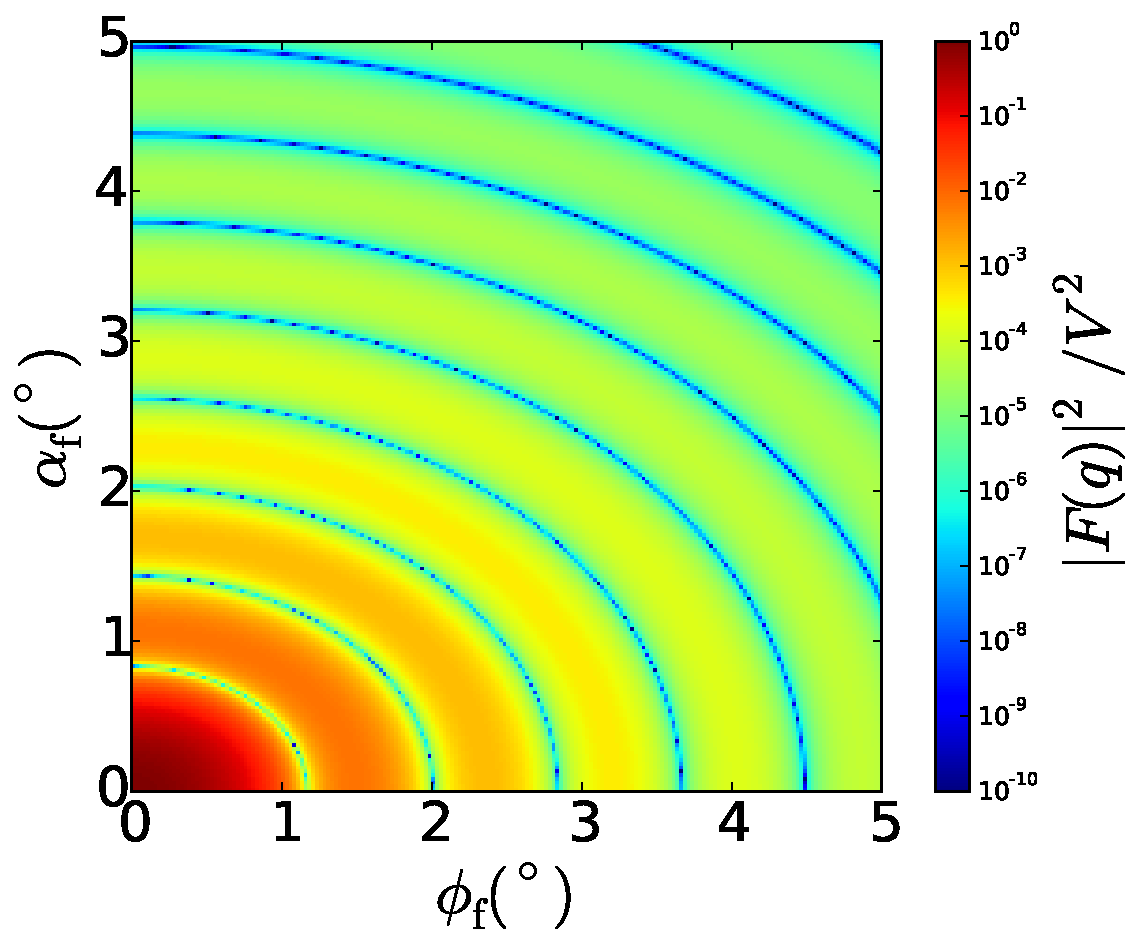
\includegraphics[width=0.5\textwidth]{fig/ff2/ff_FullSpheroid.pdf}
\end{center}
\caption{Normalized intensity $|F|^2/V^2$,
computed with $R=3.5$~nm and $H=9.8$~nm.}
% changes very little under tilt !
\end{figure}

\paragraph{History}\strut\\
Agrees with the \E{Full spheroid} form factor of \IsGISAXS\
\cite[Eq.~2.37]{Laz08} \cite[Eq.~227]{ReLL09},
with corrected volume formula.
We also discovered a wrong factor of~2 in the \IsGISAXS\ code.


%===============================================================================
\ffsection{HemiEllipsoid} \label{SHemiEllipsoid}
%===============================================================================
  \index{Hemi ellipsoid (form factor)}
  \index{Ellipsoid (form factor)!truncated}
  \index{Truncated ellipsoid (form factor)}
  \index{FormFactorHemiEllipsoid@\Code{FormFactorHemiEllipsoid}}

\paragraph{Real-space geometry}\strut\\

\begin{figure}[H]
\hfill
\subfigure[Perspective]{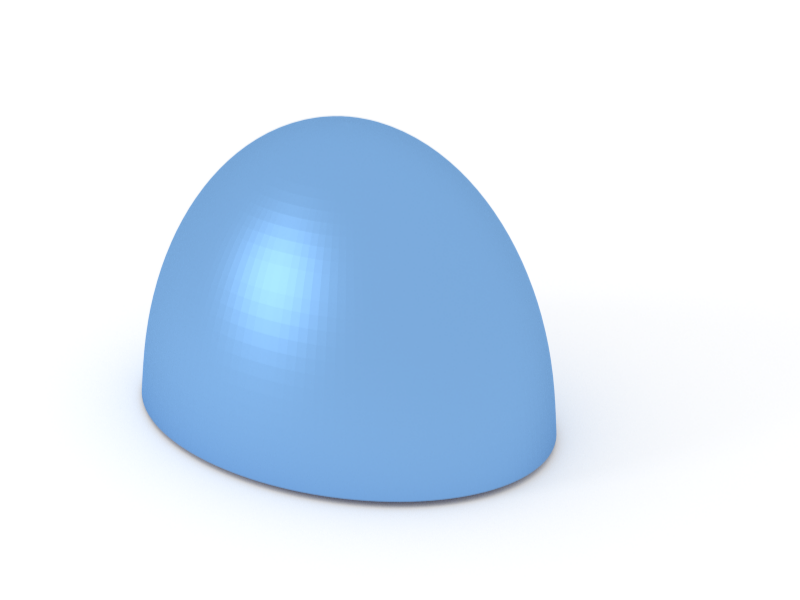
\includegraphics[width=.24\textwidth]{fig/blue/HemiEllipsoid3d.png}}
\hfill
\subfigure[Top view]{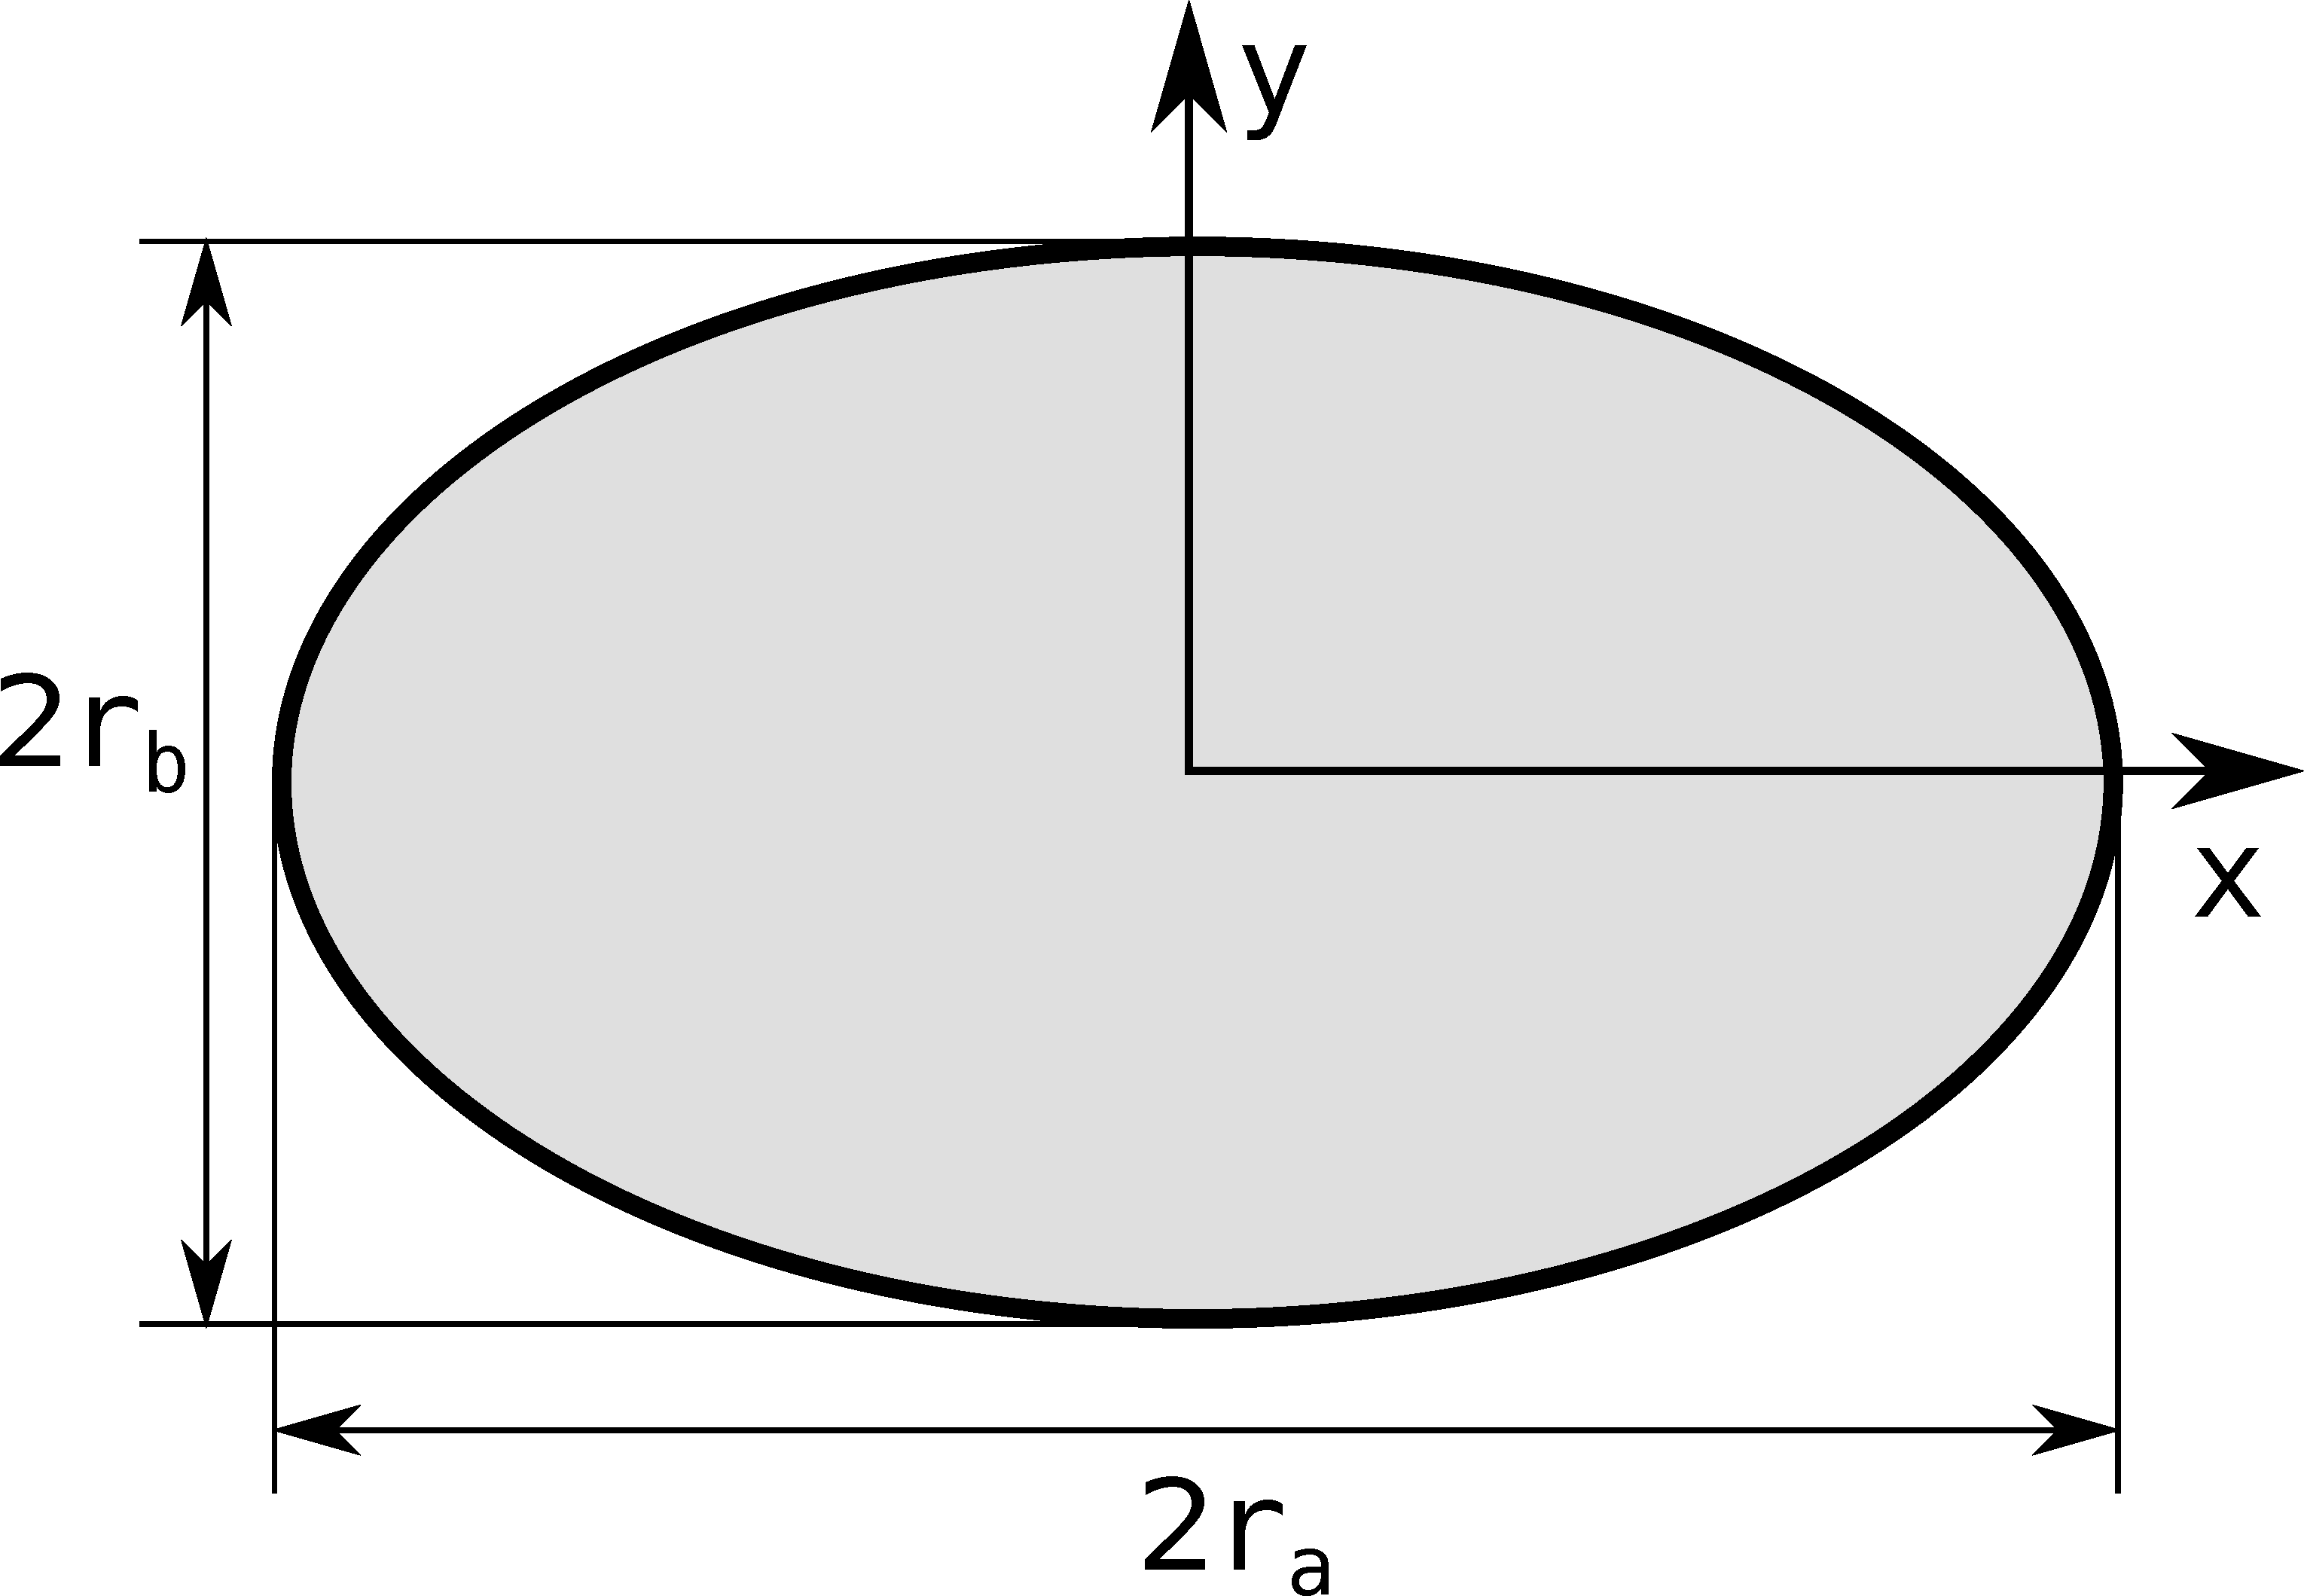
\includegraphics[width=.30\textwidth]{fig/cuts/HemiEllipsoid2dxy.pdf}}
\hfill
\subfigure[Side view]{\raisebox{5mm}{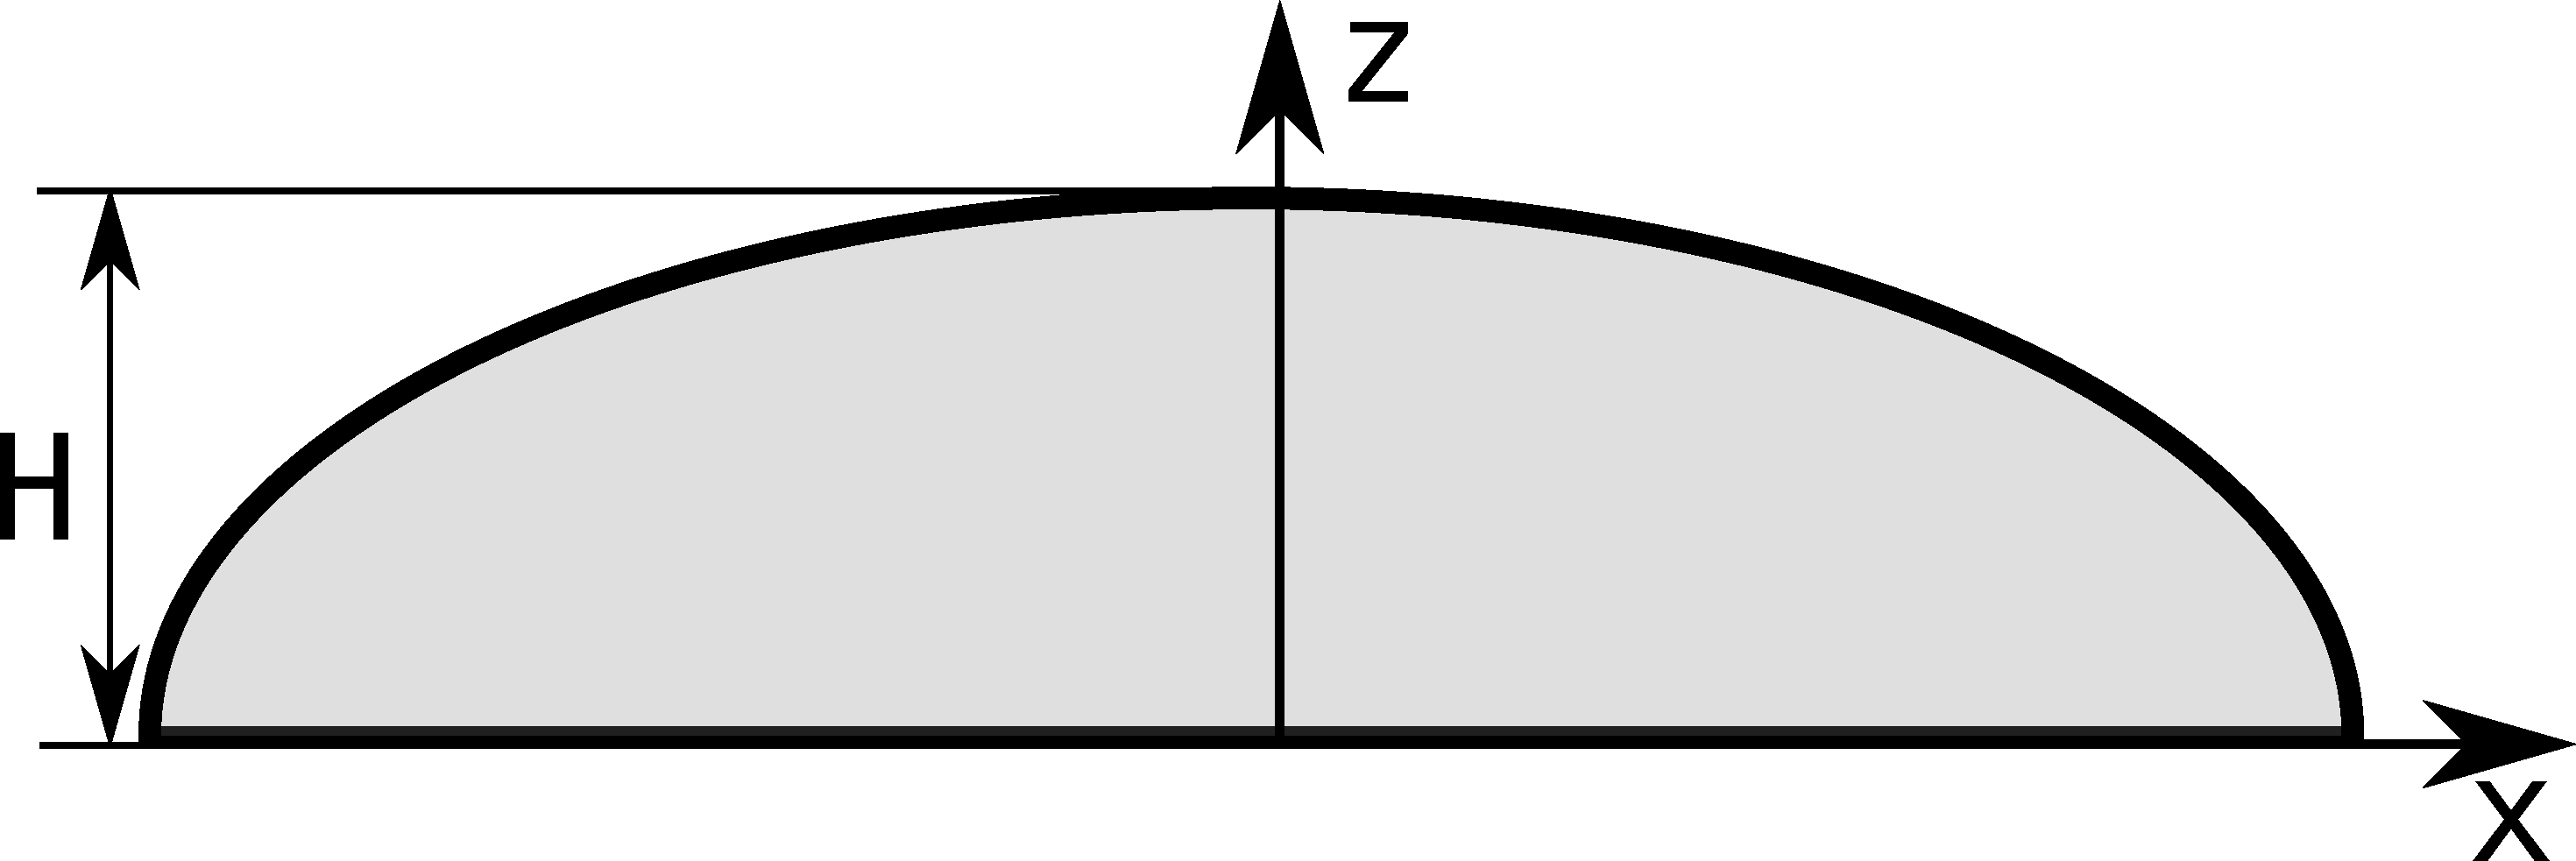
\includegraphics[width=.30\textwidth]{fig/cuts/HemiEllipsoid2dxz.pdf}}}
\hfill
\caption{An horizontally oriented ellipsoid, truncated at the central plane.}
\end{figure}

\paragraph{Syntax and parameters}\strut\\[-2ex plus .2ex minus .2ex]
\begin{lstlisting}
  FormFactorHemiEllipsoid(radius_a, radius_b, height)
\end{lstlisting}
with the parameters
\begin{itemize}
\item \texttt{radius\_a}, in $x$ direction, $R_a$,
\item \texttt{radius\_b}, in $y$ direction, $R_b$,
\item \texttt{height}, equal to radius in $z$ direction, $H$
\end{itemize}

\paragraph{Form factor, volume, horizontal section}\strut\\
Notation:
\begin{equation*}
 r_{a,z} \coloneqq R_a \sqrt{1-\left(\dfrac{z}{H} \right)^2},\quad
 r_{b,z} \coloneqq R_b \sqrt{1-\left(\dfrac{z}{H} \right)^2}, \quad
 \gamma_z =\sqrt{(q_x r_{a,z})^2+(q_y r_{b,z})^2}.
\end{equation*}
Results:
\begin{equation*}
  F = 2\pi \int_0^{H} \!\d z\, r_{a,z} r_{b,z}
                               \frac{J_1(\gamma_z)}{\gamma_z}\exp(iq_z z),
\end{equation*}
\begin{equation*}
  V = \dfrac{2}{3}\pi R_a R_bH,
\end{equation*}
\begin{equation*}
  S =\pi R_a R_b.
\end{equation*}

\paragraph{Examples}\strut

\begin{figure}[H]
\begin{center}
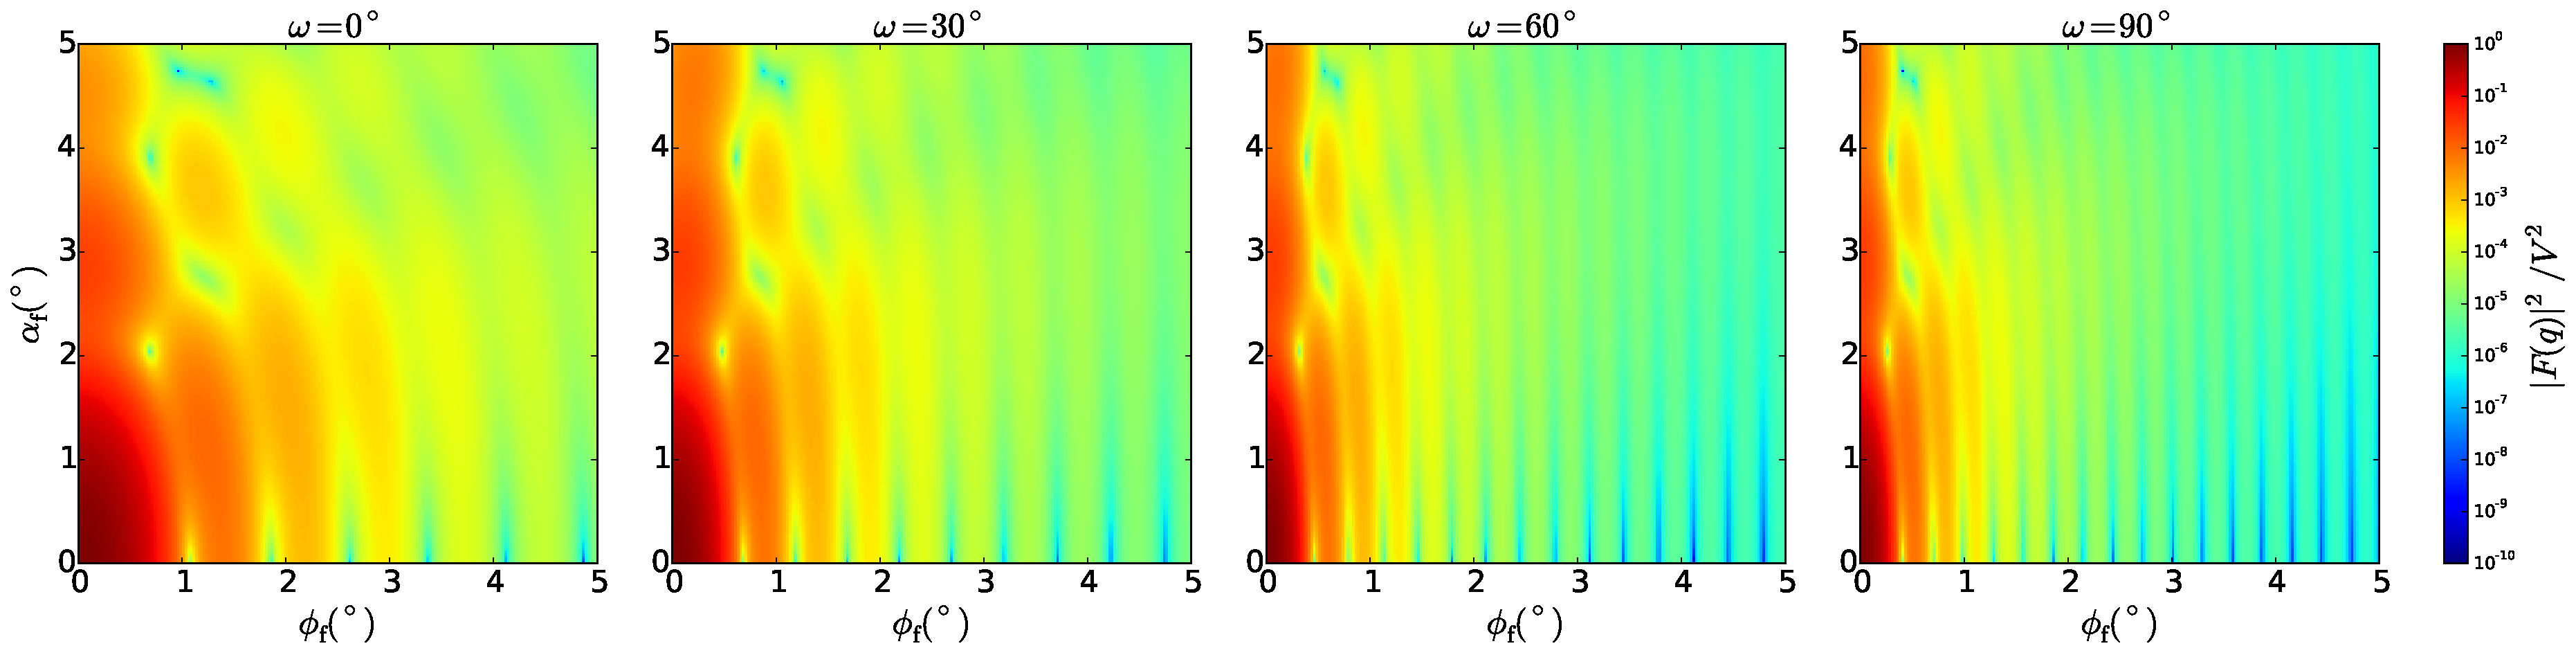
\includegraphics[width=\textwidth]{fig/ff2/ff_HemiEllipsoid.pdf}
\end{center}
\caption{Normalized intensity $|F|^2/V^2$,
computed with $R_a=10$~nm, $R_b=3.8$~nm and $H=3.2$~nm,
for four different angles~$\omega$ of rotation around the $z$ axis.}
\end{figure}

\paragraph{History}\strut\\
Agrees with the \IsGISAXS\ form factor
\E{Anisotropic hemi-ellipsoid}
\cite[Eq.~2.42, with wrong sign in the $z$-dependent phase factor]{Laz08}
or \E{Hemi-spheroid} \cite[Eq.~229]{ReLL09}.


%===============================================================================
\ffsection{Icosahedron} \label{SIcosahedron}
%===============================================================================
  \index{Icosahedron (form factor)}
  \index{Platonic solids!icosahedron}
  \index{FormFactorIcosahedron@\Code{FormFactorIcosahedron}}

\paragraph{Real-space geometry}\strut\\

\begin{figure}[H]
\strut\hfill
%\subfigure[Perspective]
{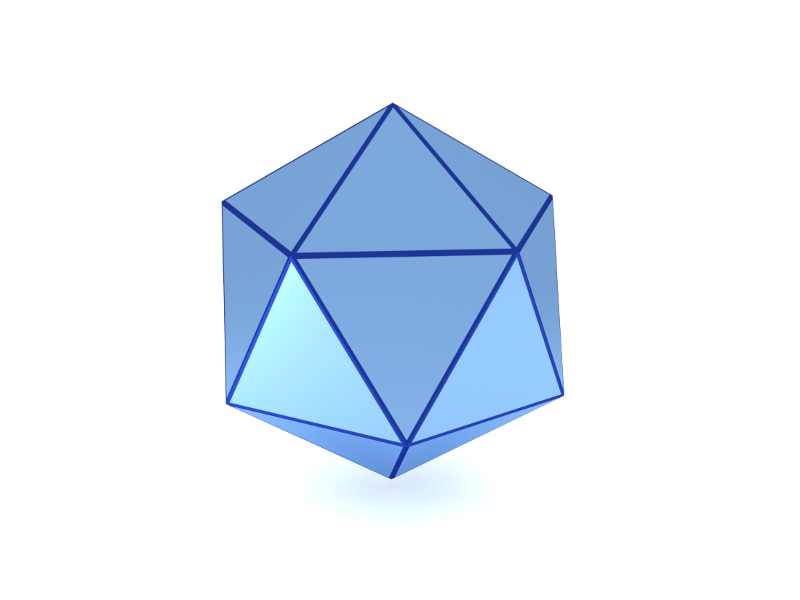
\includegraphics[width=.24\textwidth]{fig/blue/Icosahedron3d.png}}
%\hfill
%\subfigure[Top view]{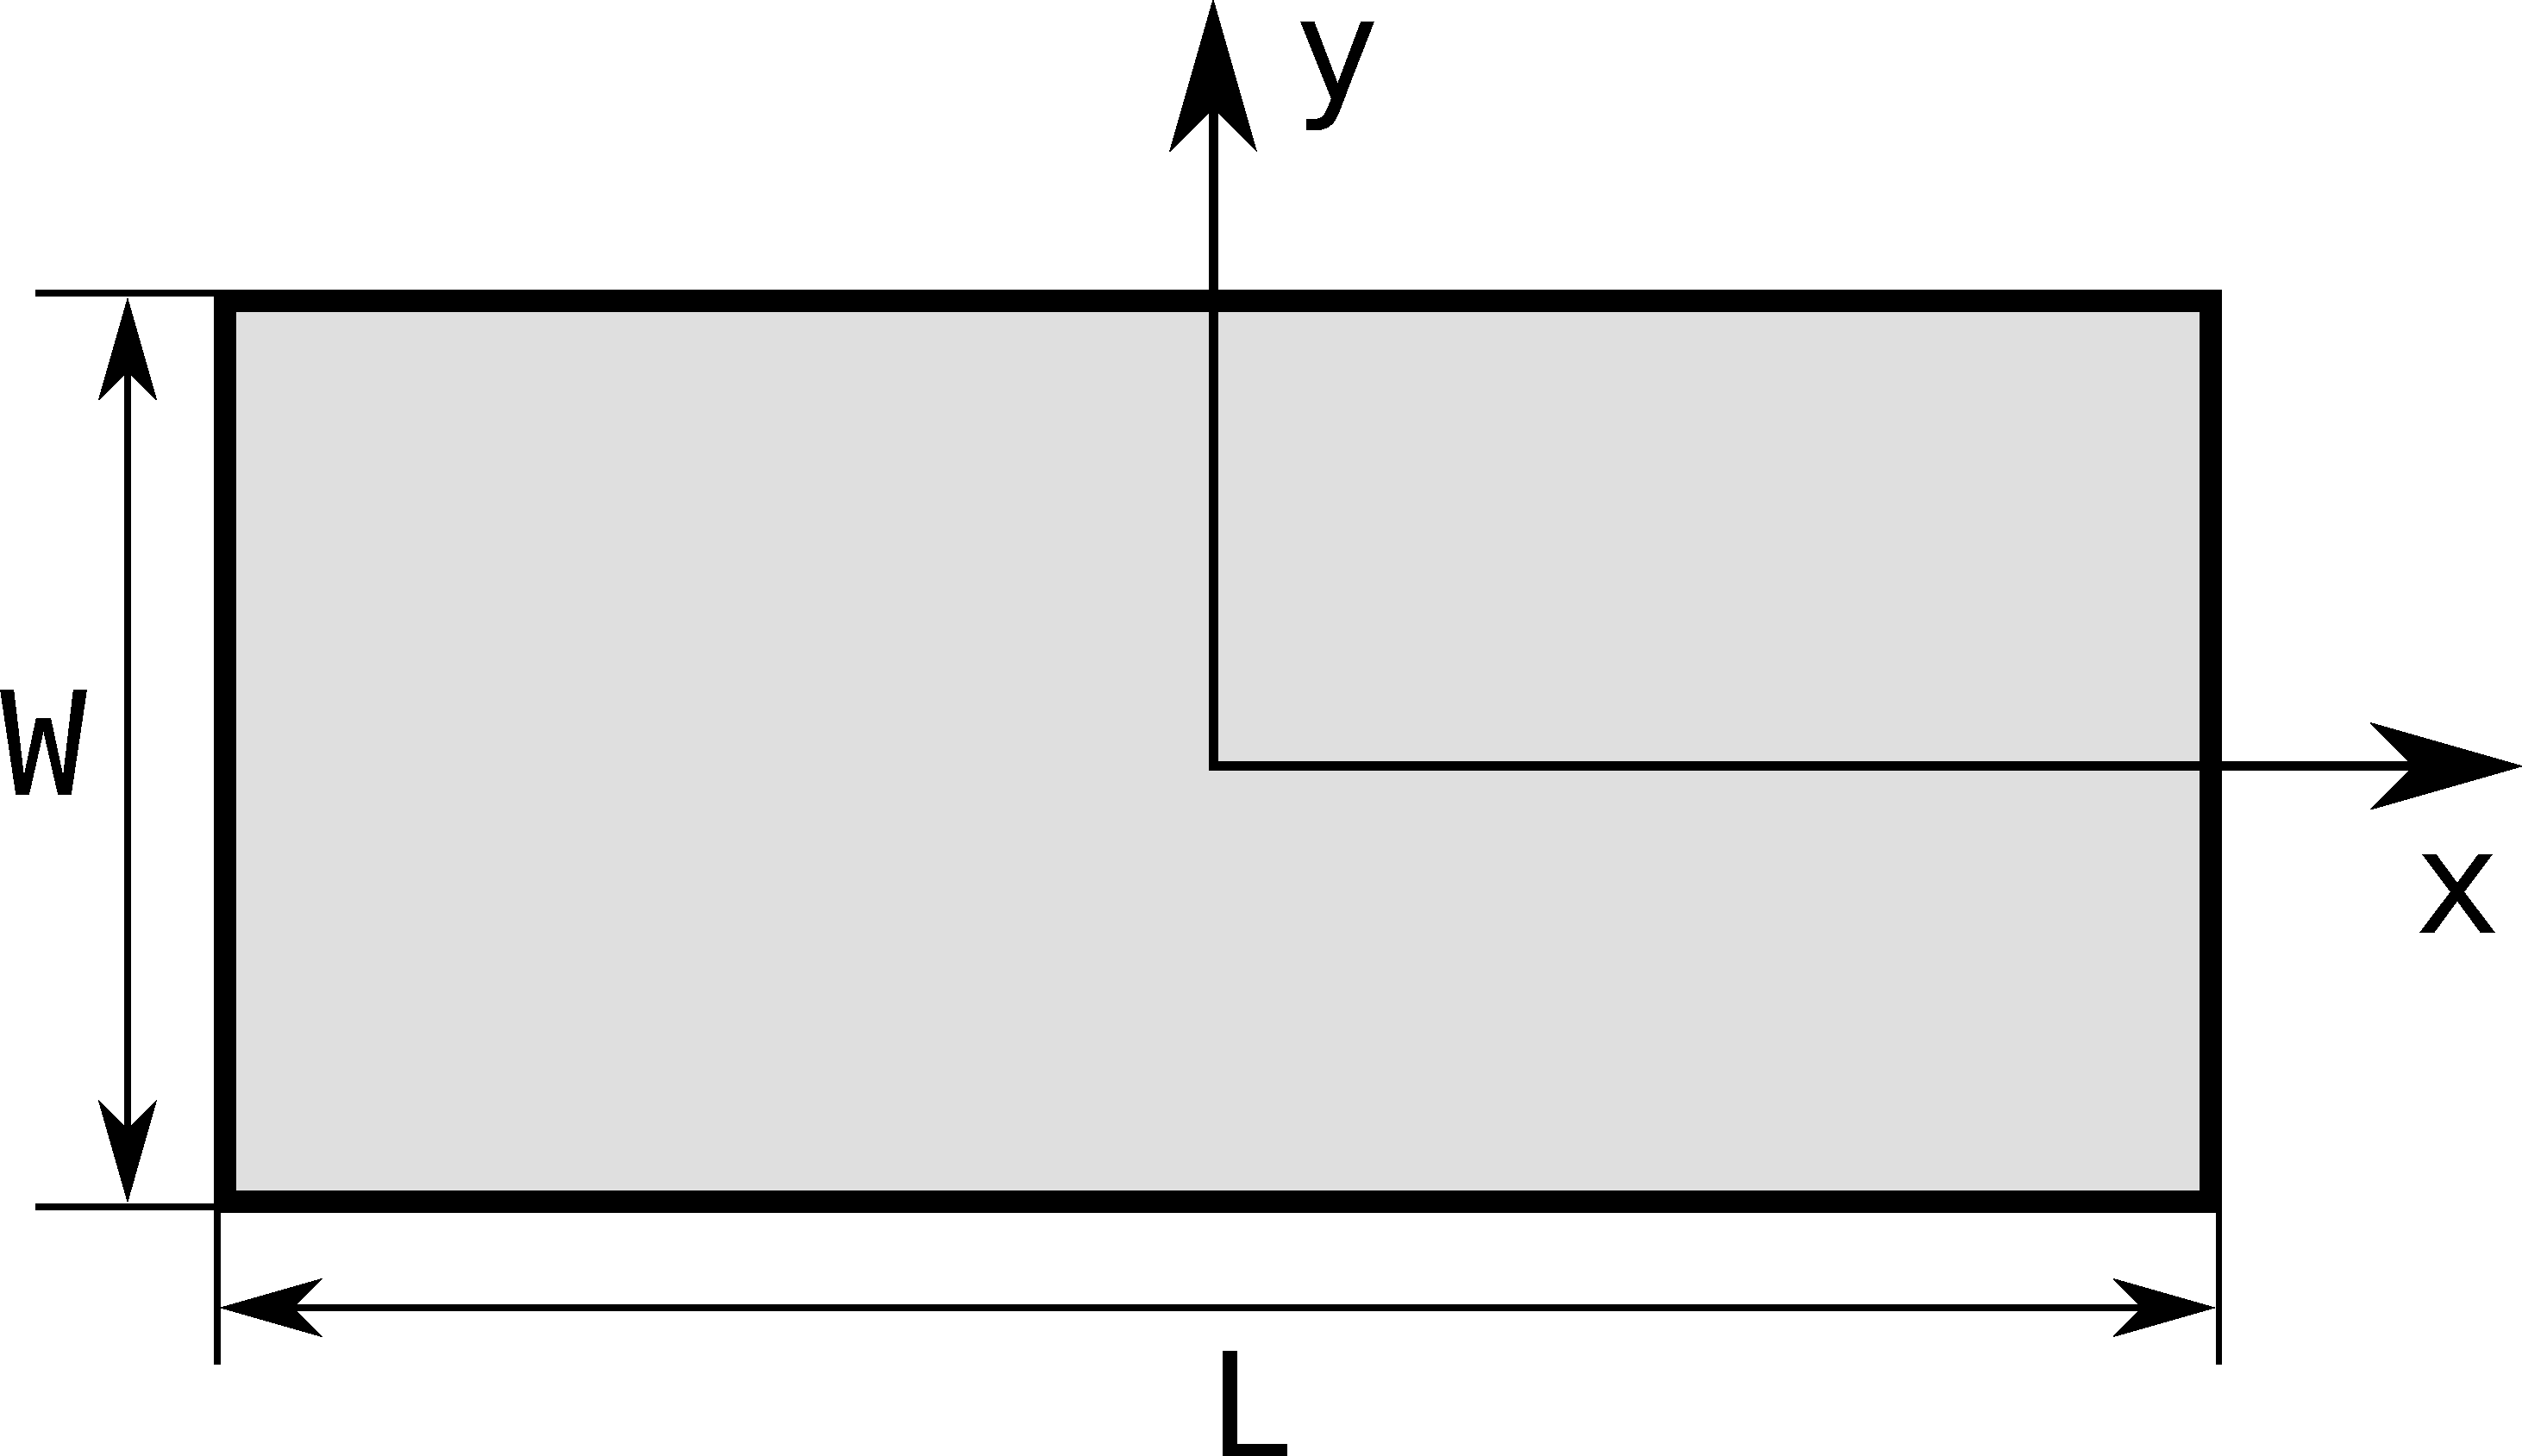
\includegraphics[width=.30\textwidth]{fig/cuts/Box2dxy.pdf}}
%\hfill
%\subfigure[Side view]{\raisebox{2mm}{\includegraphics[width=.30\textwidth]{fig/cuts/Box2dxz.pdf}}}
\hfill\strut
\caption{A regular icosahedron.}
\end{figure}

\FloatBarrier

\paragraph{Syntax and parameters}\strut\\[-2ex plus .2ex minus .2ex]
\begin{lstlisting}
  FormFactorIcosahedron(edge)
\end{lstlisting}
with the parameter
\begin{itemize}
\item \texttt{edge}, length of one edge, $a$.
\end{itemize}

\paragraph{Form factor, volume, horizontal section}\strut\\
\begin{equation*}
  F \text{~: computed using the generic form factor of a polyhedron
             with inversion symmetry~\cite{ba:ffp},}
\end{equation*}
\begin{equation*}
  V= \frac{5}{12} (3+\sqrt5)a^3 \approx 2.182\,a^3
\end{equation*}
%\begin{equation*}
%  S = %% wait for Holden, Shapes, Space, and Symmetry
%\end{equation*}

\paragraph{Examples}\strut

\begin{figure}[H]
\begin{center}
\includegraphics[width=\textwidth]{fig/ff2/ff_Icosahedron_sym.pdf}
\end{center}
\caption{Normalized intensity $|F|^2/V^2$,
computed with $a=4.8$~nm,
for three orientations of high symmetry:
$x$ axis perpendicular to a polygonal face;
vertex on the $x$ axis;
edge in the $xy$ plane and perpendicular to the $x$ axis.}
\end{figure}

\begin{figure}[H]
\begin{center}
\includegraphics[width=\textwidth]{fig/ff2/ff_Icosahedron_asy.pdf}
\end{center}
\caption{Normalized intensity $|F|^2/V^2$,
computed with $a=4.8$~nm,
for three orientations of decreasing symmetry:
base pentagon in $xy$ plane and pointing in $x$ direction;
rotated by $13^\circ$ around the $z$ axis;
ditto, and tilted by $9^\circ$ around the $x$ axis.}
\end{figure}

\paragraph{History}\strut\\
New in \BornAgain-1.6,
based on the generic form factor of the polyhedron~\cite{ba:ffp}.


%===============================================================================
\ffsection{Prism3 (triangular)} \label{SPrism3}
%===============================================================================
  \index{Prism (form factor)!triangular (Prism3)}
  \index{FormFactorPrism3@\Code{FormFactorPrism3}}

\paragraph{Real-space geometry}\strut\\

\begin{figure}[H]
\hfill
\subfigure[Perspective]{\includegraphics[width=.24\textwidth]{fig/blue/Prism33d.png}}
\hfill
\subfigure[Top view]{\includegraphics[width=.30\textwidth]{fig/cuts/Prism32dxy.ps}}
\hfill
\subfigure[Side view]{\includegraphics[width=.30\textwidth]{fig/cuts/Prism32dxz.ps}}
\hfill
\caption{A prism based on an equilateral triangle.}
\end{figure}

\FloatBarrier

\paragraph{Syntax and parameters}\strut\\[-2ex plus .2ex minus .2ex]
\begin{lstlisting}
  FormFactorPrism3(length, height)
\end{lstlisting}
with the parameters
\begin{itemize}
\item \texttt{length} of one base edge, $L$,
\item \texttt{height}, $H$.
\end{itemize}

\paragraph{Form factor, volume, horizontal section}\strut\\
\begin{equation*}
F = H \sinc\left(q_z\frac{H}{2}\right) \exp\left(-i q_z\frac{ H}{2}\right) F_\parallel(\q_\parallel)
\end{equation*}
with the form factor $F_\parallel$ of the base triangle
computed using the generic form factor of a planar polygon \cite{ba:ffp},
\begin{equation*}
  V= \dfrac{\sqrt{3}}{4} H L^2,
\end{equation*}
\begin{equation*}
  S =\dfrac{\sqrt{3}}{4}L^2.
\end{equation*}

\paragraph{Examples}\strut

\begin{figure}[H]
\begin{center}
\includegraphics[width=\textwidth]{fig/ff2/ff_Prism3.pdf}
\end{center}
\caption{Normalized intensity $|F|^2/V^2$,
computed with $L=13.8$~nm and $H=3$~nm,
for four different angles~$\omega$ of rotation around the $z$ axis.}
\label{fig:FFprism3Ex}
\end{figure}

\paragraph{History}\strut\\
Has been validated against the \E{Prism3} form factor of \IsGISAXS\
\cite[Eq.~2.29]{Laz08} \cite[Eq.~219]{ReLL09}.
Note the different parameterization $L= 2 R_{\rm{\Code{IsGISAXS}}}$.
In \FitGISAXS\ just called \E{Prism} \cite{Bab13}.
In \BornAgain-1.6,
redefined to let the $x$ axis point along a symmetry axis
(rotated by $30^\circ$ with respect to the previous version).

Reimplemented in \BornAgain-1.6 using the generic form factor
of a polygonal prism \cite{ba:ffp},
to achieve numerical stability near the removable singularity at $q\to0$.

%===============================================================================
\ffsection{Prism6 (hexagonal)} \label{SPrism6}
%===============================================================================
  \index{Prism (form factor)!hexagonal (Prism6)}
  \index{FormFactorPrism6@\Code{FormFactorPrism6}}

\paragraph{Real-space geometry}\strut\\

\begin{figure}[H]
\hfill
\subfigure[Perspective]{\includegraphics[width=.24\textwidth]{fig/blue/Prism63d.png}}
\hfill
\subfigure[Top view]{\includegraphics[width=.30\textwidth]{fig/cuts/Prism62dxy.pdf}}
\hfill
\subfigure[Side view]{\raisebox{-3mm}{\includegraphics[width=.30\textwidth]{fig/cuts/Prism62dxz.pdf}}}
\hfill
\caption{A prism based on a regular hexagon.}
\end{figure}

\FloatBarrier

\paragraph{Syntax and parameters}\strut\\[-2ex plus .2ex minus .2ex]
\begin{lstlisting}
  FormFactorPrism6(radius, height)
\end{lstlisting}
with the parameters
\begin{itemize}
\item \texttt{radius} of the hexagonal base, $R$,
\item \texttt{height}, $H$.
\end{itemize}

\paragraph{Form factor, volume, horizontal section}\strut\\
\begin{equation*}
F = H \sinc\left(q_z\frac{H}{2}\right) \exp\left(-i q_z\frac{ H}{2}\right) F_\parallel(\q_\parallel)
\end{equation*}
with the form factor $F_\parallel$ of the base hexagon
computed using the generic form factor of a planar polygon
with two-fold symmetry~($S_2$) \cite{ba:ffp},
\begin{equation*}
  V = \dfrac{3\sqrt{3}}{2}H R^2,
\end{equation*}
\begin{equation*}
  S =\dfrac{3\sqrt{3}R^2}{2}.
\end{equation*}

\paragraph{Examples}\strut\nopagebreak

\begin{figure}[H]
\begin{center}
\includegraphics[width=\textwidth]{fig/ff2/ff_Prism6.pdf}
\end{center}
\caption{Normalized intensity $|F|^2/V^2$,
computed with $R=5.7$~nm and $H=3$~nm,
for four different angles~$\omega$ of rotation around the $z$ axis.}
\label{fig:FFprism6Ex}
\end{figure}

\paragraph{History}\strut\\
Has been validated against the \E{Prism6} form factor of \IsGISAXS\
\cite[Eq.~2.31]{Laz08} \cite[Eq.~221]{ReLL09},
which has different parametrization
and lacks a factor $H$ in $F(\q)$.

Reimplemented in \BornAgain-1.5 using the generic form factor
of a polygonal prism with symmetry~$S_2$ \cite{ba:ffp},
to achieve numerical stability near the removable singularity at $q\to0$.


%===============================================================================
\ffsection{Pyramid (square-based)}\label{SPyramid}
%===============================================================================
  \index{Pyramid (form factor)!square}
  \index{Truncated pyramid (form factor)!square}
  \index{FormFactorPyramid@\Code{FormFactorPyramid}}

\paragraph{Real-space geometry}\strut\\

\begin{figure}[H]
\hfill
\subfigure[Perspective]{\includegraphics[width=.24\textwidth]{fig/blue/Pyramid3d.png}}
\hfill
\subfigure[Top view]{\includegraphics[width=.30\textwidth]{fig/cuts/Pyramid2dxy.pdf}}
\hfill
\subfigure[Side view]{\raisebox{2mm}{\includegraphics[width=.30\textwidth]{fig/cuts/Pyramid2dxz.pdf}}}
\hfill
\caption{A truncated pyramid with a square base.}
\end{figure}

\FloatBarrier

\paragraph{Syntax and parameters}\strut\\[-2ex plus .2ex minus .2ex]
\begin{lstlisting}
  FormFactorPyramid(length, height, alpha)
\end{lstlisting}
with the parameters
\begin{itemize}
\item \texttt{length} of one edge of the square base, $L$,
\item \texttt{height}, $H$,
\item \texttt{alpha}, angle between the base and a side face, $\alpha$,
\end{itemize}
They must fulfill
\begin{displaymath}
  H \le \frac{\tan\alpha}{2}L.
\end{displaymath}

\paragraph{Form factor, volume, horizontal section}\strut\\
\begin{equation*}
  F \text{~: computed using the generic polyhedron form factor~\cite{ba:ffp},}
\end{equation*}
\begin{equation*}
  V = \dfrac{1}{6}  L^3 \tan\alpha\left[ 1
             - \left(1 - \dfrac{2H}{L\tan\alpha}\right)^3 \right],,
\end{equation*}
\begin{equation*}
  S = L^2.
\end{equation*}

\paragraph{Examples}\strut

\begin{figure}[H]
\begin{center}
\includegraphics[width=\textwidth]{fig/ff2/ff_Pyramid.pdf}
\end{center}
\caption{Normalized intensity $|F|^2/V^2$,
computed with $L=10$~nm, $H=4.2$~nm and $\alpha=60^{\circ}$,
for four different angles~$\omega$ of rotation around the $z$ axis.}
\end{figure}

\paragraph{History}\strut\\
Corresponds to \E{Pyramid} form factor of \IsGISAXS\
\cite[Eq.~2.31]{Laz08} \cite[Eq.~221]{ReLL09},
except for different parametrization $L=2R_{\rm{\Code{IsGISXAXS}}}$
and a corrected sign.

Reimplemented in \BornAgain-1.6 using the generic form factor
of a polygonal prism \cite{ba:ffp},
to achieve numerical stability near the removable singularity at $q\to0$.


%===============================================================================
\ffsection{Ripple1 (sinusoidal)} \label{SRipple1}
%===============================================================================
  \index{Ripple (form factor)!sinusoidal (Ripple1)}
  \index{Sinusoidal ripple (form factor)}
  \index{FormFactorRipple1@\Code{FormFactorRipple1}}

\paragraph{Real-space geometry}\strut\\

\begin{figure}[H]
\hfill
\subfigure[Perspective]{\includegraphics[width=.24\textwidth]{fig/blue/Ripple13d.png}}
\hfill
\subfigure[Top view]{\includegraphics[width=.30\textwidth]{fig/cuts/Ripple12dxy.pdf}}
\hfill
\subfigure[Side view]{\includegraphics[width=.30\textwidth]{fig/cuts/Ripple12dyz.pdf}}
\hfill
\caption{A ripple with a sinusoidal profile.}
\end{figure}

\paragraph{Syntax and parameters}\strut\\[-2ex plus .2ex minus .2ex]
\begin{lstlisting}
  FormFactorRipple1(length, width, height)
\end{lstlisting}
with the parameters
\begin{itemize}
\item \texttt{length}, $L$,
\item \texttt{width}, $W$,
\item \texttt{height}, $H$.
\end{itemize}

The ripple is modelled as a surface
\begin{equation*}
  Z(y) = \frac{H}{2}\left[ 1 + \cos\frac{2\pi y}{W} \right].
\end{equation*}

\paragraph{Form factor}\strut\\
Using the inverse profile
\begin{equation*}
  Y(z) = \frac{W}{2\pi}\text{arccos}\left( \frac{2z}{H}-1 \right),
\end{equation*}
the form factor is computed by numeric integration:
\begin{equation*}
F = L \sinc\left(\frac{q_xL}{2}\right)
   \int_0^H\!\d z\,\e^{iq_zz}\, 2Y(z)\sinc\left(q_y Y(z)\right).
\end{equation*}
The integration is substantially accelerated by the substitution
$u=\text{arccos}( 2z/H-1)$.

\paragraph{Volume, horizontal section}\strut\\
\begin{equation*}
  V = \dfrac{L W H}{2},
\end{equation*}
\begin{equation*}
  S = L W.
\end{equation*}

\paragraph{Examples}\strut

\begin{figure}[H]
\begin{center}
\includegraphics[width=\textwidth]{fig/ff2/ff_Ripple1.pdf}
\end{center}
\caption{Normalized intensity $|F|^2/V^2$,
computed with $L=25$~nm, $W=10$~nm and $H=8$~nm,
for four different angles~$\omega$ of rotation around the $z$ axis.}
\end{figure}

\paragraph{History}\strut\\
Agrees with the \E{Ripple1} form factor of \FitGISAXS\ \cite{Bab13}.

%===============================================================================
\ffsection{Ripple2 (saw-tooth)} \label{SRipple2}
%===============================================================================
  \index{Ripple (form factor)!saw-tooth (Ripple2)}
  \index{Saw-tooth ripple (form factor)}
  \index{FormFactorRipple2@\Code{FormFactorRipple2}}

\paragraph{Real-space geometry}\strut\\

\begin{figure}[H]
\hfill
\subfigure[Perspective]{\includegraphics[width=.24\textwidth]{fig/blue/Ripple23d.png}}
\hfill
\subfigure[Top view]{\includegraphics[width=.30\textwidth]{fig/cuts/Ripple22dxy.pdf}}
\hfill
\subfigure[Side view]{\includegraphics[width=.30\textwidth]{fig/cuts/Ripple22dyz.pdf}}
\hfill
\caption{A ripple with an asymmetric saw-tooth profile.}
\end{figure}

\FloatBarrier

\paragraph{Syntax and parameters}\strut\\[-2ex plus .2ex minus .2ex]
\begin{lstlisting}
  FormFactorRipple2(length, width, height, asymmetry)
\end{lstlisting}
with the parameters
\begin{itemize}
\item \texttt{length}, $L$,
\item \texttt{width}, $W$,
\item \texttt{height}, $H$.
\item \texttt{asymmetry}, $d$.
\end{itemize}
They must fulfill
\begin{displaymath}
  |d| \le W/2.
\end{displaymath}

\paragraph{Form factor, volume, horizontal section}\strut\\
\begin{align*}
F &=L W
\sinc\left(\frac{q_xL}{2}\right)\times \\ &
\int_0^H \!\d z\,
\left(1-\frac{z}{H}\right)
 \sinc\left[\frac{q_y
    W}{2}\left(1-\frac{z}{H}\right)\right]
\exp\left\{ i\left[q_zz -
    q_yd\left(1-\frac{z}{H}\right)\right]\right\}
\end{align*}
\begin{equation*}
  V = \dfrac{L W H}{2},
\end{equation*}
\begin{equation*}
  S = L W.
\end{equation*}

\paragraph{Examples}\strut

\begin{figure}[H]
\begin{center}
\includegraphics[width=\textwidth]{fig/ff2/ff_Ripple2.pdf}
\end{center}
\caption{Normalized intensity $|F|^2/V^2$,
computed with $L=25$~nm, $W=10$~nm, $H=8$~nm, and $d=5$~nm,
for four different angles~$\omega$ of rotation around the $z$ axis.
The low symmetry requires other angular ranges than used in most other figures.}
\end{figure}

\paragraph{History}\strut\\
Agrees with the \E{Ripple2} form factor of \FitGISAXS\ \cite{Bab13}.


%===============================================================================
\ffsection{Tetrahedron} \label{STetrahedron}
%===============================================================================
  \index{Tetrahedron (form factor)}
  \index{Truncated tetrahedron (form factor)}
  \index{Platonic solids!tetrahedron}
  \index{FormFactorTetrahedron@\Code{FormFactorTetrahedron}}

\paragraph{Real-space geometry}\strut\\

\noindent
Incorrectly named so, since it actually has five, not four surfaces.

\begin{figure}[H]
\hfill
\subfigure[Perspective]{\includegraphics[width=.24\textwidth]{fig/blue/Tetrahedron3d.png}}
\hfill
\subfigure[Top view]{\includegraphics[width=.30\textwidth]{fig/cuts/Tetrahedron2dxy.ps}}
\hfill
\subfigure[Side view]{\includegraphics[width=.30\textwidth]{fig/cuts/Tetrahedron2dxz.ps}}
\hfill
\caption{A truncated pyramid, based on an equilateral triangle.}
\end{figure}

\FloatBarrier

\paragraph{Syntax and parameters}\strut\\[-2ex plus .2ex minus .2ex]
\begin{lstlisting}
  FormFactorTetrahedron(length, height, alpha)
\end{lstlisting}
with the parameters
\begin{itemize}
\item \texttt{length} of one edge of the equilateral triangular base, $L$,
\item \texttt{height}, $H$,
\item \texttt{alpha}, dihedral angle between the base and a side face, $\alpha$.
\end{itemize}
They must fulfill
\begin{displaymath}
  H\le \frac{\tan{\alpha}}{2\sqrt{3}} L.
\end{displaymath}
The orthographic projection also shows the angle~$\beta$ between the base and a side edge.
It is related to the dihedral angle through $\tan \alpha = 2 \tan \beta$.

\paragraph{Form factor, volume, horizontal section}\strut\\
\begin{equation*}
  F\text{~: computed using the generic polyhedron form factor~\cite{ba:ffp},}
\end{equation*}
\begin{equation*}
  V= \dfrac{\tan(\alpha) L^3}{24} \left[1- \left(1 -
  \dfrac{2\sqrt{3} H}{L \tan(\alpha)} \right)^3\right],
\end{equation*}
\begin{equation*}
  S =\dfrac{\sqrt{3}}{4}L^2.
\end{equation*}

\paragraph{Examples}\strut

\begin{figure}[H]
\begin{center}
\includegraphics[width=\textwidth]{fig/ff2/ff_Tetrahedron.pdf}
\end{center}
\caption{Normalized intensity $|F|^2/V^2$,
computed with $L=12$~nm, $H=8$~nm, and $\alpha=75^\circ$,
for four different angles~$\omega$ of rotation around the $z$ axis.
The low symmetry requires other angular ranges than used in most other figures.}
\end{figure}

\paragraph{History}\strut\\
Previous implementations as \E{Tetrahedron} in \IsGISAXS\
\cite[Eq.~2.30]{Laz08} \cite[Eq.~220]{ReLL09},
and as  \E{Truncated tetrahedron} in \FitGISAXS\ \cite{Bab13}.
In \BornAgain-1.6,
redefined to let the $x$ axis lay in a mirror plane
(rotated by $30^\circ$ with respect to the previous version).

Up to \BornAgain-1.5, we computed the form factor by numeric integration, as in \IsGISAXS.
Since \BornAgain-1.6 higher speed and accuracy are achieved
by using the generic polyhedron form factor \cite{ba:ffp},
with series expansions near singularities.

%===============================================================================
\ffsection{TruncatedCube} \label{STruncatedCube}
%===============================================================================
  \index{Cube (form factor)!facetted}
  \index{Facetted cube (form factor)}
  \index{FormFactorTruncatedCube@\Code{FormFactorTruncatedCube}}

\paragraph{Real-space geometry}\strut\\

\begin{figure}[H]
\hfill
\subfigure[Perspective]{\includegraphics[width=.24\textwidth]{fig/blue/TruncatedCube3d.png}}
\hfill
\subfigure[Top view]{\includegraphics[width=.30\textwidth]{fig/cuts/Truncatedcube2dxy.pdf}}
\hfill
\subfigure[Side view]{\includegraphics[width=.30\textwidth]{fig/cuts/Truncatedcube2dxz.pdf}}
\hfill
\caption{A cube whose eight vertices have been removed.
The truncated part of each vertex is a trirectangular tetrahedron.}
\end{figure}

\FloatBarrier

\paragraph{Syntax and parameters}\strut\\[-2ex plus .2ex minus .2ex]
\begin{lstlisting}
  FormFactorTruncatedCube(length, removed_length)
\end{lstlisting}
with the parameters
\begin{itemize}
\item \texttt{length} of the full cube, $L$,
\item \texttt{removed\_length}, side length of the trirectangular tetrahedron removed from the cube's vertices, $t$.
\end{itemize}
They must fulfill
\begin{displaymath}
  t \le L/2.
\end{displaymath}

\paragraph{Form factor, volume, horizontal section}\strut\\
\begin{equation*}
  F \text{~: computed using the generic form factor of a polyhedron
             with inversion symmetry~\cite{ba:ffp},}
\end{equation*}
\begin{equation*}
  V = L^3 - \dfrac{4}{3}t^3,
\end{equation*}
\begin{equation*}
  S = L^2.
\end{equation*}

\paragraph{Examples}\strut

\begin{figure}[H]
\begin{center}
\includegraphics[width=\textwidth]{fig/ff2/ff_TruncatedCube.pdf}
\end{center}
\caption{Normalized intensity $|F|^2/V^2$,
computed with $L=25$~nm, $W=10$~nm, $H=8$~nm, and $d=5$~nm,
for four different angles~$\omega$ of rotation around the $z$ axis.}
\end{figure}

\paragraph{History}\strut\\
Motivated by \cite{HeSS74}.
Reimplemented in \BornAgain-1.6 using the generic form factor
of a polygonal prism \cite{ba:ffp}.


%===============================================================================
\ffsection{TruncatedSphere}\label{STruncatedSphere}
%===============================================================================
  \index{Sphere (form factor)!truncated}
  \index{Truncated sphere (form factor)}
  \index{FormFactorTruncatedSphere@\Code{FormFactorTruncatedSphere}}

\paragraph{Real-space geometry}\strut\\

\begin{figure}[H]
\hfill
\subfigure[Perspective]{\includegraphics[width=.24\textwidth]{fig/blue/Sphere3d.png}}
\hfill
\subfigure[Top view]{\includegraphics[width=.30\textwidth]{fig/cuts/Sphere2dxy.pdf}}
\hfill
\subfigure[Side view]{\raisebox{-2mm}{\includegraphics[width=.30\textwidth]{fig/cuts/Sphere2dxz.pdf}}}
\hfill
\caption{A truncated sphere.}
\end{figure}
\FloatBarrier

\paragraph{Syntax and parameters}\strut\\[-2ex plus .2ex minus .2ex]
\begin{lstlisting}
  FormFactorTruncatedSphere(radius, height)
\end{lstlisting}
with the parameters
\begin{itemize}
\item \texttt{radius}, $R$,
\item \texttt{height}, $H$.
\end{itemize}
They must fulfill
\begin{displaymath}
   0 < H\leq 2R.
\end{displaymath}

\paragraph{Form factor, volume, horizontal section}\strut\\
Notation:
\begin{equation*}
  q_{\parallel} \coloneqq \sqrt{q_x^2+q_y^2},\quad
  R_z \coloneqq \sqrt{R^2-z^2}.
\end{equation*}
Results:
\begin{equation*}
F= 2\pi \exp[i q_z (H-R)]\int_{R-H}^{R}\!\d z\, R_z^2
       \frac{J_1(q_{\parallel} R_z) }{q_{\parallel} R_z} \exp(i q_z z) dz,
\end{equation*}
\begin{equation*}
  V=\pi R^3 \left[\dfrac{2}{3} + \dfrac{H-R}{R} - \dfrac{1}{3}\left(\dfrac{H-R}{R}\right)^3\right],
\end{equation*}
\begin{equation*}
  S = \left\{\begin{array}{ll} \pi R^2, & H \geq R \\
         \pi\left(2RH-H^2\right), & H < R \end{array}\right..
\end{equation*}

\paragraph{Example}\strut

\begin{figure}[H]
\begin{center}
\includegraphics[width=\textwidth]{fig/ff2/ff_TruncatedSphere.pdf}
\end{center}
\caption{Normalized intensity $|F|^2/V^2$,
computed with $R=4.2$~nm and $H=6.1$~nm,
for four different tilt angles~$\vartheta$ (rotation around the $y$ axis).}
\end{figure}

\paragraph{History}\strut\\
Agrees with the \IsGISAXS\ form factor
\E{Sphere} \cite[Eq.~2.33]{Laz08} or
\E{Truncated sphere} \cite[Eq.~228]{ReLL09}.


%===============================================================================
\ffsection{TruncatedSpheroid} \label{STruncatedSpheroid}
%===============================================================================
  \index{Spheroid (form factor)!truncated}
  \index{Truncated spheroid (form factor)}
  \index{FormFactorTruncatedSpheroid@\Code{FormFactorTruncatedSpheroid}}

\paragraph{Real-space geometry}\strut\\

\begin{figure}[H]
\hfill
\subfigure[Perspective]{\includegraphics[width=.24\textwidth]{fig/blue/Spheroid3d.png}}
\hfill
\subfigure[Top view]{\raisebox{5mm}{\includegraphics[width=.30\textwidth]{fig/cuts/Spheroid2dxy.pdf}}}
\hfill
\subfigure[Side view]{\includegraphics[width=.30\textwidth]{fig/cuts/Spheroid2dxz.pdf}}
\hfill
\caption{A vertically oriented, horizontally truncated spheroid.}
\end{figure}

\paragraph{Syntax and parameters}\strut\\[-2ex plus .2ex minus .2ex]
\begin{lstlisting}
  FormFactorTruncatedSpheroid(radius, height, height_flattening)
\end{lstlisting}
with the parameters
\begin{itemize}
\item \texttt{radius}, $R$,
\item \texttt{height}, $H$.
\item \texttt{height\_flattening}, $f_p$.
\end{itemize}
They must fulfill
\begin{displaymath}
  0< \dfrac{H}{R}\le 2f_p.
\end{displaymath}

\paragraph{Form factor, volume, horizontal section}\strut\\
Notation:
\begin{equation*}
  q_{\parallel} \coloneqq \sqrt{q_x^2+q_y^2}, \quad
  R_z \coloneqq \sqrt{R^2-z^2/f_p^2}.
\end{equation*}
Results:
\begin{equation*}
F =   2\pi \exp[iq_z(H-f_pR)] \int_{f_p R-H}^{f_p R} \!\d z\,
     R_z^2\frac{J_1(q_{\parallel}R_z)}{q_{\parallel}R_z} \exp(i q_z z)
\end{equation*}
\begin{equation*}
  V = \dfrac{\pi R H^2}{f_p}  \Big(1-\dfrac{H}{3f_p R}\Big),
\end{equation*}
\begin{equation*}
  S = \left\{\begin{array}{ll} \pi R^2, & H \geq f_pR \\
         \pi\left(\dfrac{2RH}{f_p}-\dfrac{H^2}{f_p^2}\right), & H < R \end{array}\right..
\end{equation*}

\paragraph{Example}\strut

\begin{figure}[H]
\begin{center}
\includegraphics[width=\textwidth]{fig/ff2/ff_TruncatedSpheroid.pdf}
\end{center}
\caption{Normalized intensity $|F|^2/V^2$,
computed with $R=3.3$~nm, $H=9.8$~nm, and $f_p=1.8$,
for four different tilt angles~$\vartheta$ (rotation around the $y$ axis).}
\end{figure}

\paragraph{History}\strut\\
Agrees with the \IsGISAXS\ form factor
\E{Sphere} \cite[Eq.~2.33]{Laz08} or
\E{TruncatedSpheroid} \cite[Eq.~228]{ReLL09}.
% Note an erroneous factor~2 in the expression of the volume
% in the \Code{IsGISAXS} manual.

\index{Shape transform!catalogue|)}
\index{Form factor!catalogue|)}
